






\documentclass[11pt,a4paper,final]{report}

\makeindex
\PassOptionsToPackage{nottoc}{tocbibind}

\usepackage{Packages/mathphdthesis}

\usepackage{acro}
\clearpage{}
\DeclareAcronym{2d}{
	short=2D,
	long=two-dimensional,
}
\DeclareAcronym{3d}{
	short=3D,
	long=three-dimensional,
}
\DeclareAcronym{a0}{
	short=A$_0$,
	long=antisymmetric fundamental Lamb wave mode,
}
\DeclareAcronym{ba}{
	short=BA,
	long=baseline algorithm,
}
\DeclareAcronym{bem}{
	short=BEM,
	long=boundary element method,
}
\DeclareAcronym{cc}{
	short=CC,
	long=correlation coefficient,
}
\DeclareAcronym{ccd}{
	short=CCD,
	long=correlation coefficient deviation,
}
\DeclareAcronym{cfrp}{
	short=CFRP,
	long=carbon fibre reinforced polymer,
}
\DeclareAcronym{cpu}{
	short=CPU,
	long=central processing unit,
}
\DeclareAcronym{di}{
	short=DI,
	long=damage index,
	plural-form=damage indices,
}
\DeclareAcronym{dau}{
	short=DAU,
	long=data acquisition unit,
}
\DeclareAcronym{dof}{
	short=DOF,
	long=degree of freedom,
	plural-form=degrees of freedom,
}
\DeclareAcronym{edif}{
	short=EDIF,
	long=experimental damage identification function,
}
\DeclareAcronym{emi}{
	short=EMI,
	long=electromechanical impedance,
}
\DeclareAcronym{eng}{
	short=ENG,
	long=damage index based on energy,
	plural-form=damage indices based on energy,
}
\DeclareAcronym{fft}{
	short=FFT,
	long=fast Fourier transform,
}
\DeclareAcronym{fdm}{
	short=FDM,
	long=finite difference method,
}
\DeclareAcronym{fem}{
	short=FEM,
	long=finite element method,
}
\DeclareAcronym{fbg}{
	short=FBG,
	long=fibre Bragg grating,
}
\DeclareAcronym{fcgm}{
	short=FCGM,
	long=full core geometry model,
}
\DeclareAcronym{gw}{
	short=GW,
	long=guided wave,
}
\DeclareAcronym{gll}{
	short=GLL,
	long=Gauss-Lobatto-Legendre,
}
\DeclareAcronym{gpu}{
	short=GPU,
	long=graphics processing unit,
}
\DeclareAcronym{hcgm}{
	short=HCGM,
	long=homogenised core geometry model,
}
\DeclareAcronym{hsc}{
	short=HSC,
	long=honeycomb sandwich composite,
}
\DeclareAcronym{ifft}{
	short=iFFT,
	long=inverse fast Fourier transform,
}
\DeclareAcronym{lisa}{
short=LISA,
long=local interaction simulation approach,
}
\DeclareAcronym{lm}{
	short=LM,
	long=Lagrange multipliers,
}
\DeclareAcronym{ncn}{
	short=NCN,
	long=National Science Centre,
}
\DeclareAcronym{madif}{
	short=MADIF,
	long=model-assisted damage identification function,
}
\DeclareAcronym{mapd}{
	short=MAPD,
	long=mean-absolute-percentage deviation,
}
\DeclareAcronym{p2p}{
	short=P2P,
	long=peak-to-peak amplitude,
}
\DeclareAcronym{pa}{
	short=PA,
	long=present algorithm,
}
\DeclareAcronym{pde}{
	short=PDE,
	long=partial differential equation,
}
\DeclareAcronym{pnn}{
	short=PNN,
	long=probabilistic neural networks,
}
\DeclareAcronym{pzt}{
	short=PZT,
	long=piezoelectric transducer,
}
\DeclareAcronym{rms}{
	short=RMS,
	long=root-mean-square,
}
\DeclareAcronym{rmsd}{
	short=RMSD,
	long=root-mean-square deviation,
}
\DeclareAcronym{s0}{
	short=S$_0$,
	long=symmetric fundamental Lamb wave mode,
}
\DeclareAcronym{sapr}{
	short=SAPR,
	long=signal amplitude peak ratio,
}
\DeclareAcronym{saps}{
	short=SAPS,
	long=signal amplitude peak-squared percentage differences,
}
\DeclareAcronym{sem}{
	short=SEM,
	long=time-domain spectral element method,
}
\DeclareAcronym{}{
	short=SEM,
	long=time domain spectral element method,
}
\DeclareAcronym{scs}{
	short=SCS,
	long=sandwich composite structure,
}
\DeclareAcronym{shm}{
	short=SHM,
	long=structural health monitoring,
}
\DeclareAcronym{sldv}{
	short=SLDV,
	long=scanning laser Doppler vibrometer,
}
\DeclareAcronym{sssd}{
	short=SSSD,
	long=signal sum of squared differences,
}
\DeclareAcronym{tof}{
	short=ToF,
	long=time of flight,
}
\clearpage{}
\usepackage[ruled,vlined]{algorithm2e}
\usepackage{multirow}
\usepackage{amsthm}
\usepackage[T1]{fontenc}
\newtheorem*{thesis*}{Thesis}
\theoremstyle{plain}
\graphicspath{{Figures/}} 

\includeonly{
Frontbackmatter/prelude 			,Frontbackmatter/newcom 			,Nomenclature/nomenclature  		,Acronyms/acronyms					,Chapters/Intro/intro  	    		,Chapters/Chapter2/ch:problem 		,Chapters/Chapter3/ch:method 		,Chapters/Chapter4/ch:sem 			,Chapters/Chapter5/ch:simulation 	,Chapters/Chapter6/ch:validation 	,Chapters/Chapter7/ch:severity 		,Chapters/Chapter8/ch:tempEffect 	,Chapters/Chapter9/ch:summary		,Appendices/app0   					,index  							}

\begin{document}

\clearpage{}

\titlepgtrue 												\signaturepagetrue 											\copyrighttrue 												\abswithesistrue 											\acktrue 													\tablecontentstrue 											\tablespagetrue 											\figurespagetrue 											

\author{\textit{Piotr Fiborek}} 	\prevdegrees{\textit{M.Sc. Eng.}}			\institute{Mechanics of Intelligent Structures Department}								

\title{\textbf{Modelling of sandwich plates and piezoelectric transducers to identify the severity of mechanical damage}}		

\submittedfor{A dissertation submitted to the Scientific Board of Institute of Fluid Flow Machinery, Polish Academy of Sciences in partial fulfillment of the requirements for the Degree of Doctor of Philosophy}			\advisor{\textit{Pawe\l{} Kudela, D.Sc. Ph.D. Eng.}} \dept{Institute of Fluid Flow Machinery, Polish Academy of Sciences}
\submitdate{Gdańsk, \textit{February, 2023}}						

\newcommand{\abstextwithesis}
{
The dissertation was aimed at developing a model-assisted method for assessing the damage in a sandwich panel with a honeycomb core. For this purpose, a structural health monitoring technique based on guided wave propagation was employed. The research offered new insight into modelling the propagation of elastic waves in a complex structure to determine how damage size affects the characteristic propagation parameters.

A function of the effect of damage size on wave propagation could be obtained by experimental investigation or theoretical analysis, but both methods are subject to certain limitations. Experimental investigation would require many expensive samples. Theoretical analysis, on the other hand, is restricted to fundamental structural elements (such as plates, bars and beams) under specific boundary conditions. In contrast, numerical modelling provides accurate data and can be flexibly adapted to different engineering structures without straining the research budget.

The numerical analysis of guided wave propagation is very time-consuming and operationally memory-intensive. Therefore, the research employed the time-domain spectral element method, one of the most accurate and efficient techniques for modelling wave propagation. The time integration algorithm was vectorised to conduct parallel computation on a multi-core graphics card. Also, computational efficiency was improved by reducing global degrees of freedom using two-dimensional elements.
Approaches to determining the material properties of composites are mainly based on the homogenisation process. However, this method is insufficient for modelling wave propagation in materials with complex structures, such as honeycomb sandwich composites. Therefore, the full core geometry model of the material structure was developed in the proposed research.

The honeycomb structure was modelled by shell spectral elements for each cell wall.
The analysis was a multiphysics approach that considered an electromechanical coupling corresponding to using piezoelectric transducers for signal excitation and sensing. The model was developed taking into account the effect of ambient temperature. In addition, to join all of the structure's components, interface elements were implemented to guarantee the continuity of the displacements of adjacent elements. A new approach was used to develop an interface based on Lagrange multipliers using spectral element shape functions to connect two non-matching grids.
The experimental measurements were conducted for model validation using (i) the impedance analyser for the piezoelectric transducers model, (ii) the scanning Doppler laser vibrometer for full-field wave propagation analysis and (iii) the piezoelectric wave acquisition setup for spot analysis of the wave propagation in the structure.

The literature review on the subject was presented at the beginning of the dissertation, alongside the description of the methodology adopted to achieve the stated purpose of the work. Then, a detailed description of the model implementation of wave propagation in a honeycomb sandwich structure using the spectral element method was presented.
Once the model had been validated, a numerical analysis was presented to determine the model-assisted damage identification function considering the varying ambient temperature. Then, parametric studies were carried out to present the effect of structural parameters on wave propagation in a honeycomb core structure. Lastly, the dissertation was summarised with conclusions arising from the analyses. 

The novelty of the research was that it developed a new approach to assessing the severity of damage and a numerical model with accurate geometry of a honeycomb structure that uses the spectral element method under varying ambient temperatures. The method that was developed could be a practical compendium of knowledge for designers of structural health monitoring.
In addition, a non-matching interface was developed to connect the two components in the frame of the spectral element method, making this technique more flexible when modelling complex structures.
}
\newcommand{\strtextwithesis}
{
Celem pracy było opracowanie wspomaganej modelem metody oceny uszkodzeń mechanicznych w płycie warstwowej z rdzeniem o strukturze plastra miodu. W tym celu zastosowano technikę monitorowania stanu technicznego konstrukcji opartą na propagacji fal prowadzonych. Badania umożliwiły nowe spojrzenie na modelowanie propagacji fal sprężystych w złożonej strukturze w celu określenia, jak rozmiar uszkodzenia wpływa na charakterystyczne parametry propagacji.

Funkcja wpływu wielkości uszkodzenia na propagację fali mogłaby być uzyskana poprzez badania eksperymentalne lub analizę teoretyczną, ale obie metody podlegają pewnym ograniczeniom. Badania eksperymentalne wymagałyby wielu kosztownych próbek. Analiza teoretyczna, z drugiej strony, jest ograniczona do podstawowych elementów konstrukcyjnych (takich jak płyty, pręty i belki) w określonych warunkach brzegowych. Natomiast modelowanie numeryczne dostarcza dokładnych danych i można elastycznie dostosować do różnych struktur inżynierskich bez nadwyrężania budżetu badań.

Analiza numeryczna propagacji fali kierowanej jest bardzo czasochłonna i wymaga znacznych zasobów pamięci operacyjnej. Dlatego zastosowano metodę elementów spektralnych w dziedzinie czasu, która jest jedną z najdokładniejszych i najbardziej wydajnych technik modelowania propagacji fal sprężystych. Algorytm całkowania w czasie został zwektoryzowany w celu prowadzenia obliczeń równoległych na wielordzeniowej karcie graficznej. Zwiększono również efektywność obliczeniową poprzez redukcję globalnych stopni swobody stosując elementy dwuwymiarowe.

Podejścia do wyznaczania właściwości materiałowych kompozytów opierają się głównie na procesie homogenizacji. Metoda ta jest jednak niewystarczająca do modelowania propagacji fal w materiałach o złożonej strukturze, takich jak kompozyty warstwowe o strukturze plastra miodu. Dlatego w proponowanych badaniach opracowano model struktury materiału o pełnej geometrii rdzenia. Struktura plastra miodu została zamodelowana za pomocą powłokowych elementów spektralnych dla każdej ściany komórki rdzenia.

W analizie zastosowano podejście wielofizyczne, w którym uwzględniono sprzężenie elektromechaniczne odpowiadające zastosowaniu przetworników piezoelektrycznych do wzbudzania i rejestrowania sygnału. Model został opracowany z uwzględnieniem wpływu temperatury otoczenia. Dodatkowo, w celu połączenia wszystkich elementów struktury, zaimplementowano elementy interfejsowe gwarantujące ciągłość przemieszczeń sąsiednich elementów. Do opracowania interfejsu zastosowano nowe podejście oparte na mnożnikach Lagrange'a wykorzystujące funkcje kształtu elementów spektralnych do połączenia dwóch niepasujących siatek.

W celu walidacji modelu przeprowadzono pomiary eksperymentalne z wykorzystaniem (i) analizatora impedancji dla modelu przetworników piezoelektrycznych, (ii) skanującego wibrometru laserowego Dopplera do analizy pełnego pola propagacji fali oraz (iii) piezoelektrycznego zestawu akwizycji fal do punktowej analizy propagacji fal w strukturze.

Przegląd literatury przedmiotu został przedstawiony na początku rozprawy, gdzie opisano również metodologię, która została przyjęta do realizacji założonego celu pracy. Następnie przedstawiono szczegółowy opis realizacji modelu propagacji fali w strukturze warstwowej o strukturze plastra miodu z wykorzystaniem metody elementów spektralnych.
Po walidacji modelu przedstawiono analizę numeryczną mającą na celu wyznaczenie funkcji identyfikacji uszkodzeń wspomaganej modelem z uwzględnieniem zmiennej temperatury otoczenia. Następnie przeprowadzono badania parametryczne w celu przedstawienia wpływu parametrów płyty z rdzeniem o strukturze plastra miodu na propagację fali. Na koniec podsumowano rozprawę, przedstawiając wnioski wynikające z przeprowadzonych analiz. 

Nowatorskość przeprowadzonych badań polegała na opracowaniu nowego podejścia do oceny stopnia uszkodzenia oraz modelu numerycznego z dokładną geometrią rdzenia o strukturze plastra miodu wykorzystując metodę elementów spektralnych w warunkach zmiennej temperatury otoczenia. Opracowana metoda może stanowić praktyczne kompendium wiedzy dla projektantów systemów monitorowania stanu technicznego konstrukcji. Ponadto, w ramach metody elementów spektralnych, opracowano interfejs do połączenia dwóch sąsiednich elementów o niepasujących siatkach, co czyni tę technikę bardziej elastyczną przy modelowaniu złożonych struktur.
}

\newcommand{\acknowledgement}
{
}

\newcommand{\engineeringquote}
{
\null\vfill
\begin{quote}
"When you want to know how things really work, \\  \hspace*{2cm} study them when they’re coming apart."\begin{flushright}- William Gibson 
\end{flushright}
\end{quote}
\vfill
}

\renewcommand{\bibname}{Bibliography}
\setlength\bibitemsep{1.5\itemsep}

\newcolumntype{L}[1]{>{\raggedright\let\newline\\\arraybackslash\hspace{0pt}}m{#1}}
\newcolumntype{C}[1]{>{\centering\let\newline\\\arraybackslash\hspace{0pt}}m{#1}}
\newcolumntype{R}[1]{>{\raggedleft\let\newline\\\arraybackslash\hspace{0pt}}m{#1}}

\beforepreface
The realisation of the dissertation would not have been possible without the support and encouragement of many people.
First and foremost, I would like to express my gratitude to my thesis supervisor Professor Paweł Kudela for his guidance and perceptive view of my thesis.
I am fortunate to have grown my interests and research career with him.

I would like to thank Professor Wiesław Ostachowicz, head of the Centre of Mechanics of Machinery and the Mechanics of Intelligent Structures Department.
It is a great honour to be a member of the team pioneering research in structural health monitoring.
I also thank Professor Alfred Zmitrowicz, Head of Doctoral Studies at the Institute of Fluid-Flow Machinery.
I am also grateful to Professor Maciej Radzieński and Professor Tomasz Wandowski for sharing their enormous knowledge of laser vibrometer and electromechanical impedance measurements, respectively.

Moreover, I wish to thank all the Mechanics of Intelligent Structures Department researchers who supported me with their knowledge and professional experience during theoretical and experimental work: Prof. Grzegorz Zboiński, Prof. Katarzyna Majewska, Prof. Paweł Malinowski, Prof. Magdalena Mieloszyk, Dr Shirsendu Sikdar, Dr Rohan Soman and Kaleeswaran Balasubramaniam.

I would acknowledge the Polish National Science for financial support under grant agreement no. 2018/31/N/ST8/02865 and Renata Opieka-Sowińska and Monika Ratajczak for administrative services of the project.

I wish to thank all my friends and family who supported me until the end of my dissertation writing.
Special thanks go to my parents, who passed on what is most important in life.

Last but not least, I would like to acknowledge my beloved girls, my wife Honorata, and my daughters Hanna and Emilia, for their continuous support throughout the dissertation preparation.
\afterpreface\clearpage{}
\clearpage{}

\newtheorem{theorem}{Theorem}[section]
\newtheorem{lemma}[theorem]{Lemma}
\newcommand{\bfx}{{\ensuremath{\mathbf{x}}}}
\clearpage{}
\clearpage{}

\chapter*{Nomenclature}
\addcontentsline{toc}{chapter}{Nomenclature}
\label{nomenclature}










\printnomenclature[6em]
\clearpage{}
\clearpage{}

\chapter*{Acronyms}
\addcontentsline{toc}{chapter}{Acronyms}
\label{acronyms}
\printacronyms[heading=none,pages={display=first}]\clearpage{}
\clearpage{}\pagenumbering{arabic}



\chapter[Introduction]{Introduction}
\label{ch:intro}
The dissertation is the result of the author’s work as an assistant in the Department of Mechanics of Intelligent Structures, Institute of Fluid Flow Machinery, Polish Academy of Sciences.
Most of the work was carried out within the framework of a research project titled ‘Model-assisted damage identification function for Structural Health Monitoring of composite structures under a varied environmental condition', which was granted to the author by the National Science Centre, Poland.
The primary objective was to develop a new approach to a sandwich structure assessment based on guided waves techniques under varied operating conditions.
The essence of the proposed method was to establish an accurate and numerically efficient model of the wave propagation in the sandwich structure, which allowed for determining the mechanical damage severity.
A better understanding of guided wave behaviour in such structures and their interaction with damage may allow the development of more precise structural health monitoring strategies, reducing costs without compromising the safety of the liable systems.


\section{Sandwich composite structure}
\label{sec:scs}

Composites consist of two or more different materials, such as plastics, resins, metal alloys, glass, carbon or bio-based fibres. The combination of material constituents gives  structure benefits from the properties of the component materials, e.g., the strength of carbon fibres and the low density of the polymer resin in the case of \ac{cfrp}.
The contribution of lightweight composite materials to the production of structural components has been increasing rapidly since the middle of the last century.
Composite materials are extensively used in aircraft, aerospace and civil constructions due to their high strength-to-weight ratio, high operating temperatures, great stiffness and high reliability.
For example, composites account for more than 50\% of the total weight of the aircraft Boeing 787 and Airbus A350 \cite{giurgiutiu2015structural}.

One group of composites includes sandwich panels, a multi-layered structure consisting of a mid-core attached between thin shells.
The skins, made of high-strength materials, are designed to carry tensile or compressive stresses from longitudinal forces and bending moments.
On the other hand, the core transmits mainly shear stresses from transverse forces.
It also separates the skins, which increases structural stiffness for thin layers, improves insulation properties, and reduces weight while maintaining strength properties similar to the solid construction of the same density.
A popular core used in engineering structures is a honeycomb geometry core. 
The typical \ac{hsc} is shown in Figure~\ref{fig:hcp}.
The core is composed of lightweight materials, the most common of which include aluminium, cardboard or Nomex\textsuperscript{\tiny\textregistered}.
\begin{figure}[H] \begin{center}
		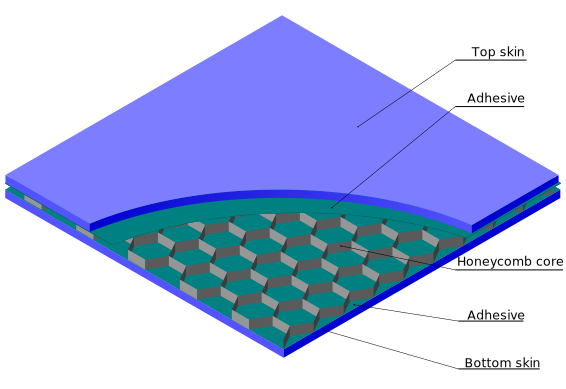
\includegraphics[width=0.95\textwidth]{Intro/honeycomb_plate}
		\caption{
			\label{fig:hcp} Structure of the honeycomb sandwich composite}
		\vspace{-0.5cm}
	\end{center}
\end{figure}

However, various types of damage can occur in these complex structures not found in metal alloy materials. These types of damage include hidden disbonds of the skin and core, delamination of composite skins, or impact damage to the core.
Damage can appear during manufacturing, storage, and operation, so online defect detection methods are required.
Therefore, the increased use of composite materials in the industry has motivated the development of advanced approaches to structural inspections, e.g., methods based on elastic wave propagation had to account for the anisotropic structure of the material. \section{Structural health monitoring}
\label{sec:scm}

\Ac{shm} is the process of implementing an advanced damage identification strategy for structural or mechanical systems \cite{farrar2007introduction}.
The \ac{shm} systems usually consist of a sensor network, a \ac{dau}, and a central processor.
The \ac{dau} is responsible for collecting the data measured by the sensor network.
A central unit then determines the current state of the structure through signal processing and statistical classification.
The main goal of \ac{shm} is to increase structure safety use through the ability to observe crucial components in real time. 
The main goal of \ac{shm} is to increase structure safety use through the ability to observe crucial components in real time.
Since advanced \ac{shm} methods are also applied to structures made of lightweight composite materials, the economic aspect is improved in addition to safety.
For example, composites and adhesive bonding techniques reduce the aircraft's weight and fuel consumption \cite{scelsi2011potential}.
The \ac{shm} is most commonly found in structures, such as aerospace, civil and mechanical engineering, where damage can have catastrophic consequences.

Rytter, in his dissertation \cite{rytter1993vibrational}, classified the \ac{shm} system advancement into the following four levels:
\begin{itemize}
	\item[] \textbf{Level 1}: Detection,
	\item[] \textbf{Level 2}: Localisation,
	\item[] \textbf{Level 3}: Assessment,
	\item[] \textbf{Level 4}: Consequence.
\end{itemize}
The first level determines if any adverse change in the geometry or material characteristics of the system has occurred.
The second level leads to the localisation of the damage.
The two most advanced levels of the system determine the size of the flaw and decide whether any maintenance is necessary, respectively.
The existence and location of faults can be defined in unsupervised learning mode by taking a threshold value for a measurable, damage-sensitive system feature. The threshold should be compensated depending on the prevailing operational and environmental conditions.
In contrast, damage size is determined in supervised learning mode based on an analytical model or data extracted experimentally from the structure \cite{worden2007fundamental}. \section{Piezoelectric transducers}
\label{sec:PZT}

The piezoelectric phenomenon is the generation of an electrical charge on the surface of materials under mechanical deformation in crystalline materials with no inversion symmetry.
The magnitude of the generated charge is proportional to the strain and the direction of polarization.
Those materials also exhibit the opposite effect: a change in size due to an applied electric field.
Piezoelectric materials are widely used in engineering as electroacoustic transducers, high voltage generators and power sources, energy harvesters, micro motors and actuators.
\begin{figure}[H]
	\begin{center}
		\includegraphics[width=0.95\textwidth]{Intro/PZTs}
	\end{center}
	\caption{Various types of piezoelectric transducers (\textbf{a}) circular discs, (\textbf{b}) circular array of the transducers, (\textbf{c}) Smart Layer\textsuperscript{\tiny\textregistered} sensors - piezoelectrics embedded into dielectric film manufactured by Acellent Technologies, Inc.}
	\label{fig:piezo}
\end{figure}
The \acp{pzt}, the acronym derived from the chemical formula of the most commonly used piezoelectric ceramic, i.e. Pb[Zr\(_x\)Ti\(_{1-x}\)]O\(_3\) (lead zirconate titanate), are lightweight, various size and shape structures.
Examples of ready-to-use \ac{pzt} are shown in Figure~\ref{fig:piezo}.
They can be permanently mounted on the structure surface, embedded within the material, or even be a smart composite material.
In the \ac{shm}, they are mainly used in elastic wave propagation, modal analysis, and the \ac{emi} methods. \section{Selected \acl{shm} techniques using the \aclp{pzt}}
\label{sec:techniques}



\subsection{Guided waves based techniques}

\begin{figure}[!htb]
	\begin{center}
		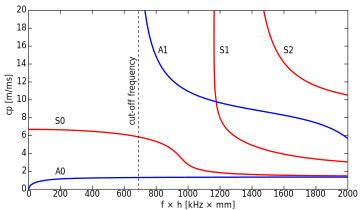
\includegraphics[width=0.95\textwidth]{Intro/dispersion}
	\end{center}
	\caption{Dispersion diagram for a 1 \unit{\mm} \acs{cfrp} plate (adopted from Dispersion Calculator~\cite{huber2021dispersion}). Red and blue solid curves represent symmetric and antisymmetric modes, respectively; a black dashed line indicates the cut-off frequency for higher modes}
	\label{fig:dispersion}
\end{figure}
\Acp{gw} are mechanical waves being a superposition of shear and longitudinal waves propagating in a bounded elastic medium, e.g., bars, beams, rods, plates and shells. 
Guided waves are multi-modal and dispersive, i.e. more than one mode travels simultaneously through the medium with the phase velocity depending on the frequency.
Figure~\ref{fig:dispersion} shows an example of dispersion curves generated by the Dispersion Calculator~\cite{huber2021dispersion} software for a 1 \unit{\mm} thick \ac{cfrp} plate in the frequency range of 0-2000 \unit{\kHz}.
\Ac{a0} and \ac{s0}, considering the distribution of particle displacements on the upper and lower free surface relative to a central surface, are observed for low frequencies.
The mode shapes are pictured in Figure~\ref{fig:mode_shape}, with the \ac{s0} particle displacements being dominant in-plane, while the \ac{a0} is dominated by out-of-plane motion.
Moreover, higher harmonic modes appear over the cut-off frequency, as shown in Figure~\ref{fig:dispersion}.

\begin{figure}[!htb]
	\begin{center}
		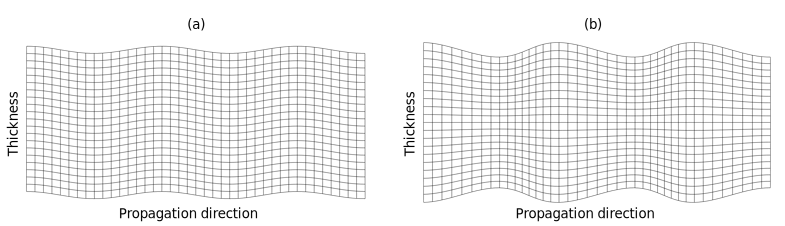
\includegraphics[width=0.95\textwidth]{Intro/mode_shape}
	\end{center}
	\caption{Mode shape of the (\textbf{a}) \acl{a0} and (\textbf{b}) \acl{s0} at 100 \unit{\kHz} in 2 \unit{\mm} composite plate (exported from Dispersion Calculator~\cite{huber2021dispersion})}
	\label{fig:mode_shape}
\end{figure}

Detection schemes based on \acp{gw} exploit reflection, attenuation, and mode conversion when the propagating wave encounters a discontinuity in the structure \cite{alleyne1992interaction}.
Thus, this technique is efficient in detecting various types of defects, such as delamination \cite{sohn2011delamination,tian2015delamination}, adhesive disbonds \cite{rucka2018damage,balasubramaniam2021ultrasonic}, corrosion changes \cite{alleyne1995long,lowe1998defect}, cracks \cite{tua2004detection,lu2006crack,zima2020detection} and failures in \acp{hsc} \cite{mustapha2011assessment, sikdar2016guided, sikdar2016ultrasonic,radzienski2016assessment, yu2019core}.
Many techniques based on \ac{gw} propagation have been developed for damage detection and localisation.
A pitch-catch technique \cite{ihn2008pitch, sikdar2017structural} uses a pair of sensors; one excites, and the other receives a signal.
If the wave encounters a defect between the sensors, it will scatter, and the recorded signal will be distorted.
In the case of the pulse-echo technique \cite{guo1993interaction, kudela2008damage}, there is one sensor that excites the wave and, at the same time, registers possible echoes from the damage.
The damage distance from the transducer can be determined if the wave speed is known and the \ac{tof} is measured.
Moreover, defect localisation can be determined if at least three sensors are used.
The radar principles were utilized in a phased array technique for plate inspection \cite{giurgiutiu2004embedded, ostachowicz2008elastic, kudela2018structural}.
The technique uses an array of transducers, each excited with an appropriate time offset, to focus all the waves at a single grid point of the area to be inspected.
A damage map is determined once the signals are obtained and processed for the entire grid.
Fink proposed a different approach, which is known as a time-reversal mirror technique \cite{fink1992time}.
In this method, the wave propagates from one sensor to another, and then after time-reversal and dispersion compensation, the wave is re-emitted to the origin sensor.
The resulting signal will be a mirror image of the forcing signal only if the wave does not encounter damage \cite{park2007time, eremin2016analytically}.

The \acp{pzt} can be used mutually as actuator-receiver pairs or as a single actuator with other devices, e.g. the \ac{sldv}, \ac{fbg} sensors.
The \acp{pzt} generate high forces with broadband frequency, so methods based on \ac{gw} can detect various damage types of different sizes in a large inspected area.
Moreover, specific algorithms do not require a baseline model, and the method implementation is economically efficient.

\subsection{Electromechanical impedance methods}
The \ac{emi} spectroscopy is also an effective and powerful technique in the \ac{shm} for real-time structural damage assessment \cite{park2003overview}.
The basis of this method is the influence of the mechanical impedance of the inspected host structure on the electrical impedance of the \ac{pzt} attached to the structure.
Assuming that the mechanical property of the sensor remains unchanged over the monitoring period, any changes in measurements of the electrical impedance can be considered a difference in the structure stiffness, which in turn can indicate that a defect has occurred.

Fundamentals of the \ac{emi} method were introduced by Liang et al. \cite{liang1994impedance}.
An analytical model of the \ac{pzt} actuator bonded to one end of a single degree of freedom mass-spring-damper system was presented in this pioneering work.
In the early papers, the authors adopted quasi-static sensor approximation until  Giurgiutiu and Zagrai \cite{giurgiutiu2000characterization} derived an expression where the sensor dynamics were incorporated.
The dynamics of a single \ac{pzt} with various boundary conditions (free, clamped and elastically constrained) and a sensor attached to a beam were considered.
Further investigation was performed for the sensor bonded to the host structures \cite{zagrai2001electro, giurgiutiu2005damage}.
Damage detection was realised by comparing the state of the structure with the reference state using overall statistical damage indices, e.g., the \ac{rmsd}, the \ac{mapd}, \ac{ccd} and \ac{pnn}.
Malinowski et al. \cite{malinowski2014characterisation, malinowski2015use} investigated the effects of \ac{emi} changes related to the state of the adhesive layer between two composite plates.
The technique evaluated weak bonds due to inadequate adhesive curing temperature, release agent and moisture contamination.
This type of damage was not detectable using the method based on \ac{gw} propagation.
Experimental testing was conducted on weakened samples and compared with a reference.
The \ac{rms} of the conductance in the range of 3-5 MHz and the first thickness resonant frequency shift were considered for bond-line assessment.

An and Sohn \cite{an2012integrated} proposed a new damage detection technique that combines \ac{emi} and \ac{gw} advantages.
In the method, measured admittance characteristic was separated into two parts: active and passive.
\Ac{di} was a weighted sum of two indicators obtained from \ac{gw} signal and active admittance.
Because passive impedance is only sensitive to temperature variation, it was used for temperature compensation on both mentioned signals.
Instead of two \acp{di}, Sevillano et al. \cite{sevillano2016damage} proposed a more integrated \ac{di} based on the electromechanical power dissipation of the \ac{pzt} sensor.

The \ac{emi} technique can detect damage, such as delamination or cracks, but is also sensitive to changes, such as weak bonds, which the \ac{gw} method is ineffective at detecting.
However, the \ac{emi} is a local method for high frequency.
Giurgiutiu et al. \cite{giurgiutiu2001electro} obtained consistent results for crack detection in distances up to 40 \unit{\mm} from the sensor in the frequency range of 300-450 \unit{\kHz}.
The use of broad-band high-frequency signals sparks difficulties in preparing a reasonable and efficient numerical model.
In addition, a homogenised model of composite materials may be inadequate because short-wavelength modes interact with the reinforcing fibres.
This method is also sensitive to environmental conditions such as temperature and humidity fluctuations \cite{bhalla2002practical} or loading variations \cite{lim2011impedance}. \section{Challenges in \acl{gw} propagation modelling for damage assessment in \acl{hsc}}
\label{sec:challenges}

Assessing the damage severity in structural materials requires a database of the damage influence on system response \cite{worden2007fundamental}.
In the case of \ac{hsc}, many factors affect the \ac{di} magnitude, such as damage localisation, material properties and dimensions, the sensor position relative to the core cell and the boundary conditions.
Determining \ac{di} by experimental means becomes very complicated, expensive and time-consuming, considering all the factors.
Therefore, numerical analysis and computer simulations become the only practical tool to achieve the goal.

The most common \ac{hsc} numerical model used in analysing \acp{gw} and \ac{emi} found in the literature is based on the \ac{fem}.
Although the numerical results are close to the experimental results, the models have some limitations in performing the simulations with reasonable computation time and operating memory consumption.
In order to alleviate these limitations, the techniques are employed as follows:
\begin{itemize}
\item reduction of the sample dimensions \cite{hosseini2013numerical, tian2015wavenumber},
\item homogenisatin of the core properties \cite{catapano2014multi, zhou2020debonding},
\item a simplified \ac{2d} model based on a cross-section of the panel~ \cite{li2019detection},
\item omission of an adhesive layer \cite{mustapha2013non}.
\end{itemize}

The time and memory consumption of the \ac{fem} simulations is due to the high spatial resolution needed to converge the numerical results.
When first-order elements are used, up to 20 nodes per the shortest wavelength of interest is recommended by Moser et al. \cite{moser1999modeling}.
At a time when the operational capabilities of personal computers were severely limited, several methods derived from classic \ac{fem} were developed to increase the efficiency of calculations.
The \ac{bem} has been widely used for wave propagation in infinite or semi-infinite areas \cite{brebbia1984boundary}.
This method uses the fundamental solution of a \ac{pde} with the approximation only at the boundary of the domain.
The \ac{fdm} also has found application in elastic wave modelling \cite{delsantoO1992connection}.
The solution of the \ac{pde} is realised by the Taylor expansion with the arbitrary number of terms that determines the order of accuracy \cite{willberg2015simulation}.
The main disadvantage of this method is the loss of numerical stability for the structure with varying material properties.

To avoid this drawback, Delsanto et al. developed the \ac{lisa} with the combination of a sharp interface model to connect to different domains \cite{delsantoO1992connection}. This method is the extension of the \ac{fdm} in which iteration equations are obtained directly from heuristic consideration \cite{willberg2015simulation}.
The \ac{lisa} is highly numerically efficient because local interactions between elements are directly transferred for numerical calculations.

However, no usage of the \ac{bem}, \ac{fdm} and \ac{lisa} in \ac{hsc} modelling has been documented in the literature, supposedly due to the complex geometry of the core.
Realistic shape of the core can be implemented while keeping numerical efficiency using a technique based on high-order elements.
The implementations of this technique have been developed in recent years, achieving convergence even at six nodes in case of \ac{gw} propagating in isotropic plates \cite{willberg2012comparison}.
One of the implementations is a method based on Lagrange polynomials as a shape function and the \ac{gll} for integration scheme, termed the \ac{sem}.
The \ac{sem} was initially developed for the numerical solution of the fluid flow in a channel by Patera \cite{patera1984spectral}.
The method has also been successfully employed for acoustic wave propagation in geological structures \cite{seriani1994spectral, komatitsch2000simulation} and \ac{gw} propagation in engineering elements \cite{kudela2007wave, ostachowicz2011guided, rucka2010experimental,rekatsinas2017cubic}.
The \ac{sem} can be applied to complex structures, e.g. stiffened panels \cite{schulte2011simulation, lonkar2014modeling}.
The versatility of the method is also related to the use of hybrid elements in combination with \ac{fem} formulation \cite{ha2009optimizing} and non-linear issues \cite{yu2020time, li2021hybrid}.

Due to the fast convergence and flexibility of the \ac{sem}, Kudela \cite{kudela2016parallel} applied the method to the \ac{hsc} model with the \ac{fcgm}.
However, the author used \ac{3d} elements to model the core walls resulting in a huge number of \acp{dof}.
The model size could be reduced if the shell element replaced the solid one.
In addition, the surface-mounted \ac{pzt} is omitted in the above model, and a concentrated force is used as the disturbance source.
The sensor mesh would have to coincide with the plate mesh or use the coupling between both meshes to include the \acp{pzt} in the simulation.
Such coupling can be realised using an interface based on Lagrange multipliers proposed by Farhat and Roux for domain decomposition in \ac{fem} \cite{farhat1991method}.
Ashwin et al. implemented the interface for the \ac{sem} but did not adopt it to non-matching grids \cite{ashwin2014formulation}, which is required to generalise the model.
Therefore, one of the goals of the dissertation was to implement a non-matching grid approach for the \ac{sem}.

Besides a computationally efficient model, an important factor affecting the speed of computer simulations is the hardware on which they are performed.
Recently, the use of \ac{gpu}-equipped workstations in numerical computation has grown.
However, to employ the \ac{gpu} for calculations, the time integration algorithm must be prepared for parallel processing.
The implementation of the algorithm for the \ac{sem} was presented by Kudela \cite{kudela2016parallel} and by Paćko et al. for the \ac{lisa} \cite{packo2012lamb}.
According to \cite{kudela2016parallel}, the multi-core architecture of the \ac{gpu} enables simultaneous vector operations, making simulations over 14 times faster than those performed by a \ac{cpu}.
Determining the effect of damage size for models with a large number of \ac{dof} should be done using the \ac{gpu} to perform a series of simulations in a reasonable amount of time. 
\section{Conclusions}
\label{sec:conclusionsIntro}

The Introduction briefly reviewed issues raised in the dissertation, i.e., composite materials, their construction and applications; definition of the \ac{shm} and application of the \ac{pzt} sensors in damage detection; and challenges in \ac{gw} propagation modelling for damage severity assessment in \acp{hsc}.

According to the literature review, a useful method for damage size assessment in \ac{hsc} is needed to enhance the safety of using composite structures.
In the dissertation, a novel approach for assessing the size of mechanical damage in a sandwich panel was proposed and developed using a \ac{gw} propagation technique.
This procedure involved actuation of elastic waves in the investigated structure, as well as their recording with the use of the \ac{pzt} setup.
The signals and a preliminary numerical analysis that defined a function of the impact of damage on wave propagation were used to estimate the defect severity.
The milestone of the dissertation was to prepare numerically effective model of \ac{gw} propagation in a sandwich panel.
The selection process of a suitable numerical modelling technique addressed the following issues:
\begin{itemize}
	\item flexibility to model the complex structure of the honeycomb core
	\item time efficiency due to the large number of \ac{dof} in the model
	\item possibility of parallel calculation on the \ac{gpu}.
\end{itemize}\clearpage{}
\clearpage{}



\chapter[Problem Statement]{Problem Statement}
\label{ch:problem}





Composite materials are used as structural components whose failure can have catastrophic consequences.
Although \ac{gw}-based methods are promising for damage detection and localisation, they have not been widely reported to estimate damage size.
A better understanding of the effect of damage on elastic wave propagation in the \acp{hsc} may allow the development of robust and practical tools to evaluate this structure.

The principal aim of this dissertation was to propose a new approach for damage severity identification in \ac{hsc} employing the \acp{pzt}.
The essence of the method was the determination of damage influence function on characteristic parameters of the propagating waves in the structure.
This function was defined using a numerical model developed using the \ac{sem}.

Initially, the model was prepared for the healthy sample.
Then parametric simulations for various damage size were performed.
The \ac{madif} was determined based on the obtained results. 
This function determines the flaw size depending on the \acp{pzt} response.
For the purposes of the research, debonds of the core and the skin were considered as damage.
The \ac{madif} was also determined at various ambient temperatures.

The objectives of the dissertation were as follows:
\begin{itemize}
	\item develop a robust and efficient numerical model of the propagating \ac{gw} in \ac{hsc} with the temperature as an additional parameter
	\item validate the model experimentally
	\item determine the \ac{madif} to define damage influence on the propagating waves
	\item investigate the \ac{madif} under various ambient temperatures
	\item study the effects of various \ac{hsc} parameters on the \ac{madif}.
\end{itemize}

The presented objectives leaded to the thesis formulated as follows:
\begin{thesis*}  
	Model-assisted analysis of guided wave propagation is an effective tool for determining the damage severity in honeycomb sandwich composites.
\label{thesis}
\end{thesis*}

Chapter~\ref{ch:method} presents the methods for developing a model-assisted damage severity assessment scheme.

Chapter~\ref{ch:sem} gives a theoretical background of the \ac{sem} for \ac{gw} propagation.
It includes the derivation of mass, stiffness and damping matrices for 2D and 3D formulation; interface coupling algorithm; time integration scheme; and parallel implementation for GPU calculation.

Chapter~\ref{ch:simulation} details the sample configuration for the \ac{fcgm} and the \ac{hcgm}.
The meshing process of individual components of the \ac{shm} system, signal parameters and the damage model is presented.

The results of numerical simulations and experimental validation are presented in Chapter~\ref{ch:validation}.

The crucial part of the dissertation appears in Chapter \ref{ch:severity}.
Based on the performed simulations and their experimental validation, the function of the damage size effect on the elastic wave propagation in \ac{hsc} was established, termed \ac{madif}.

Chapter~\ref{ch:tempEffects} includes the analysis of \ac{gw} propagation under variable temperature conditions.

The conclusion of the dissertation and final remarks are provided in Chapter~\ref{ch:summary}.

\clearpage{}
\clearpage{}

\chapter[Concept of the Method]{Concept of the Method}
\label{ch:method}

The Chapter presents the research methodology used in the dissertation to determine the validity of the thesis. 
First, a discussion of different methods for numerical modelling \ac{gw} propagation in \ac{hsc} is provided. 
Then a framework of the new model is presented, complemented by the description of methods for determining the material properties of each component for varied ambient temperatures.
The Chapter also describes the proposed model-assisted damage severity assessment approach.
\section{Modelling of \acl{gw} propagation in \aclp{hsc}}
\label{sec:modelling}





In the dissertation, the \ac{hsc} structure consists of an aluminium honeycomb core and one skin made of \ac{cfrp}.
The most common numerical modelling of the phenomenon of \ac{gw} in \acp{hsc} found in the literature is a calculation of the effective material properties of the honeycomb structure \cite{baid2015dispersion, mustapha2014leaky, qi2008ultrasonic,  shi1995derivation, sikdar2016guided}.
The properties are obtained from the analytical \cite{gibson1982mechanics, malek2015effective} or the \ac{fem} \cite{catapano2014multi, chen2014analysis} analysis of the honeycomb representative volume element.
A comprehensive literature review on the homogenisation of the honeycomb structure is presented in the work of Ahmed \cite{ahmed2019homogenization}.
Replacing the core geometry with a homogeneous material has many advantages.
First and foremost, it simplifies the domain mesh, therefore convergence of the solution requires less operational memory and increases the value of the time step.
In addition, the wave propagation velocity determined by the simulation is in good agreement with the experiment.

However, this method cannot adequately represent the phenomenon of propagating wave interaction in honeycomb cells.
It causes the signal energy not to dissipate as it would in a real structure.
A more precise model is the \ac{fcgm}. 
Ruzzene~et~al. presented a parametric study to evaluate the dynamic behaviour of the honeycomb and cellular structures through the \ac{fem} and the application of the theory of periodic structures \cite{ruzzene2003wave}.
Recently, wave propagation simulations in \acp{hsc} have been conducted with commercially available finite element software~\cite{song2009guided, hosseini2013numerical, tian2015wavenumber, zhao2018wave}.

While the \ac{fem}-based modelling of \ac{gw} requires a significant amount of memory and it is time-consuming, this method becomes inefficient in the case of \ac{fcgm}.
Kudela increased the computational efficiency with the model based on the \ac{sem} \cite{kudela2016parallel}.
In addition, the algorithm has been adapted for parallel computing on the \ac{gpu}, making the simulations 14 times faster than on the \ac{cpu}.
However, this approach has two major disadvantages. Firstly, it employed solid elements with three \acp{dof} per node to model the core walls. As a result, a \numproduct{179 x 160} \unit{\square\mm} sandwich panel had over 1.5 million \acp{dof}.
Secondly, no \ac{pzt} sensors were considered in the simulation, so a concentrated force was used to generate the \ac{gw}.
To include the sensor in the simulation, the sensor mesh must coincide with the grid of the host plate, or a joining interface between them must be used.

The drawbacks of previous modelling methods motivated me to propose a new \ac{hsc} model.
In this study, the \ac{sem} was used to develop the \ac{fcgm}, in which each core wall was modelled with \ac{2d} elements.
It significatly simplified the core mesh compared to the implementation using \ac{3d} elements.
Since the neutral plane of the elements is oriented differently concerning the global coordinate system, the local displacements vector has to be transformed accordingly.
The transformation was carried out after introducing the sixth degree of freedom, which is a rotation regarding the out-of-plane axis and using the directional cosines vector of the element.
The \ac{cfrp} skin plate was modelled with the \ac{3d} elements and the material properties were homogenised according to the laminate theory presented by Vinson and Sierakowski \cite{vinson1993behavior}.
Solid elements were also used for modelling the \acp{pzt}.
The thin adhesive layers were considered as an isotropic material and modelled with the \ac{2d} elements.
In addition, two interfaces were used to connect all \ac{hsc} components together.
One with the non-matching grid was developed to join the sensors with the skin.
For this purpose a new approach was implemented based on the element shape functions.
The core and skin connection was implemented with a perfectly matching interface.
The presented model has not been found in the literature and the details of the implementation are presented in Chapter \ref{ch:sem}.

The parametric study conducted in the dissertation leaded to the determination of a \ac{madif}, which defines the effect of damage size on wave propagation.
In this case, the defect was assumed to be disbonds of the skin and the core. \section{Temperature effect on \acl{gw} propagation}
\label{sec:temp}
 
The high propagation velocities of \acp{gw} make a single measurement last about 1-2 microseconds.
Compared to slow changes in ambient temperature (in seconds), the propagation phenomenon can be modelled for the stationary temperature field.
It was assumed that the temperature field can be obtained from temperature sensors at the moment of \ac{gw} excitation.
For simplicity, the model assumed a uniform temperature field.

According to \cite{lu2005methodology, kijanka2013gpu}, there are two main factors that influence how temperature affects the Lamb waves propagation. First, the thermal expansion of the plate causes the propagation path to be extended. As the coefficient of thermal expansion of the \ac{cfrp} is relatively low (-0.76 \unit[per-mode = symbol]{\micro\meter\per\kelvin} in longitudinal direction along the reinforcing fibres \cite{ahmed2012study}) it was neglected in the consideration.
The other is the temperature dependence of wave velocity due to the variation in material properties of the components.
In the presented models, only changes in the elastic modulus of \ac{hsc} components were considered, while the density changes were neglected.
The mechanical properties of the considered \ac{hsc} components at the reference temperature \(T_r=20\)\unit{\degreeCelsius} are included in Table~\ref{tab:properties}.
\begin{table}[H]
	\small
	\tabcolsep=0.5cm
	\centering
	\caption{\label{tab:properties}The mechanical properties of the materials at a reference temperature of +20\unit{\degreeCelsius}}
	\begin{tabular}{ccccc}\toprule
		\multirow{2}{*}{\textbf{Material}} & $\boldsymbol{E_{11}}$ & $\boldsymbol{E_{33}}$ & $\boldsymbol{\nu_{12}}$ & $\boldsymbol{\rho}$ \\ & \unit{\giga\pascal} & \unit{\giga\pascal} & -- & \unit[per-mode = symbol]{\kilogram\per\cubic\meter}\\
		\midrule
		Carbon & 275 & 27 & 0.2 & 1900\\
		Epoxy & 3.43 & 3.43 & 0.35 & 1250\\
		Aluminium & 69 & 69 & 0.33 & 2770\\
		Epoxy adhesive & 6 & 6 & 0.34 & 1200\\
		Cyanoacrylate glue & 3 & 3 & 0.34 & 1200\\	
		\ac{pzt} &  59 & 47 & 0.31 & 7850\\
		\bottomrule
	\end{tabular}
\end{table}
Young's modulus for the \ac{cfrp} skin was calculated accordingly to the methodology described in \cite{chamis1983simplified, salamone2009guided, sikdar2018effects}.
The significant changes in mechanical properties under temperature occur mainly in the polymer matrix, while the variation in the carbon fibre properties has a negligible effect on wave propagation.
In this model \cite{salamone2009guided, hopkins2012extreme}, the reduction of Young’s modulus of the resin \(E_m\) with temperature variation was assumed as
\begin{eqnarray}
	E_m(T)=F_m E_{m}(T_r),
	\label{eq:factor_temp}
\end{eqnarray}
\nomtypeR[E]{$E$}{Young's modulus}{}{\unit{\giga\pascal}}\nomtypeR[T]{$T$}{Temperature}{}{\unit{\degreeCelsius}}\nomtypeR[Tr]{$T_r$}{Reference temperature}{}{\unit{\degreeCelsius}}where \(E_{m}(T_r)\) is Young’s modulus of the resin at the reference temperature, and \(F_m\) is the temperature degradation factor.
According to \cite{chamis1983simplified}, it equals
\begin{eqnarray}
F_m=\sqrt{\frac{T_{g0}-T}{T_{g0}-20}},
\label{eq:em_temp}
\end{eqnarray}
\nomtypeD[Fm]{$F_m$}{Temperature degradation factor}{}\nomtypeR[Tg0]{$T_{g0}$}{Glass transition temperature}{}{\unit{\degreeCelsius}}where \(T_{g0}\) is the glass transition temperature.
Effective temperature-dependent properties of the \ac{cfrp} skin are presented in Figure \ref{fig:cfrpEG}.
The values of Young's modulus along and across carbon fibres, \(E_{11}\) and \(E_{33}\), respectively are depicted in Figure \ref{fig:cfrpEG}(\textbf{a}), and shear modulus \(G_{12}\) and \(G_{23}\) in Figure \ref{fig:cfrpEG}(\textbf{b}).

\begin{figure}
	\begin{center}
		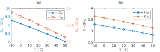
\includegraphics[width=0.95\textwidth]{Chapter_3/cfrpEG}
	\end{center}
	\caption{Temperature-dependent (\textbf{a}) Young's modulus (E\(_{11}\), E\(_{33}\)) and (\textbf{b}) shear modulus (G\(_{12}\), G\(_{23}\)) for the \acs{cfrp} skin}
	\label{fig:cfrpEG}
\end{figure}

Equation (\ref{eq:em_temp}) is also applicable to determine the elastic modulus of the adhesive layer.
The linear temperature dependence for aluminium given by Hopkins~et~al.~\cite{hopkins2012extreme} is defined as
\begin{eqnarray}
	E_a(T)=E_a(T_{r})+\num{4e7}(20-T).
	\label{eq:aluminium_temp}
\end{eqnarray}

Temperature-dependent properties of isotropic materials were determined according to the formulas and the fact that shear and Young's modulus are in relation as \(E=2G(1+\nu)\).
Young's modulus and shear modulus are presented in Figure \ref{fig:isoEG}(\textbf{a}) and Figure \ref{fig:isoEG}(\textbf{b}), respectively, for aluminium, adhesive layer and cyanoacrylate glue.
\begin{figure}
	\begin{center}
		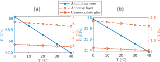
\includegraphics[width=0.95\textwidth]{Chapter_3/isoEG}
	\end{center}
	\caption{Temperature-dependent (\textbf{a}) Young's modulus (E) and (\textbf{b}) shear modulus (G) for isotropic materials used in the simulations}
	\label{fig:isoEG}
\end{figure}

Young's modulus and Poisson's ratio of the sensors were in the form proposed by Lanza et al. \cite{lanza2008temperature}
\begin{eqnarray}
	\left(E_{11}\right)_{pzt}(T) & = & \left[\left(E_{11}\right)^{-1}_{pzt}(T_r) + \num{2.142857e-14}(20-T)\right]^{-1},\\
	\left(E_{33}\right)_{pzt}(T) & = & \left[\left(E_{33}\right)^{-1}_{pzt}(T_r) + \num{0.777142e-14}(20-T)\right]^{-1},\\
	\nu_{pzt}(T) & = & \nu_{pzt}(T_r) + \num{13e-3}(20-T).
	\label{eq:pzt_temp}
	\nomtypeD[nu]{\( \nu \)}{Poisson's ratio}{}
\end{eqnarray}

The piezo- and electromechanical properties were taken into account based on the
temperature characteristics provided by the manufacturer.
\begin{figure}
	\begin{center}
		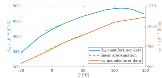
\includegraphics[width=0.95\textwidth]{Chapter_3/pzt_piezo_temp}
	\end{center}
	\caption{Temperature-dependent charge constant (\(d_{33}\)), and electric permittivity (\(\epsilon_{33}\)) of the \acs{pzt} provided by the manufacturer}
	\label{fig:pzt_temp}
\end{figure}
Due to the values provided by the manufacturer being in \(\pm10\%\) tolerance, the characteristics were approximated by the linear functions in the analysed range (see Figure \ref{fig:pzt_temp}) given in the form
\begin{eqnarray}
	\textbf{d}(T) & = & \boldsymbol{d}(T_r) + \left[
	\begin{array}{cccccc}
		0 & 0 & 0 & 0 & 0 & 0\\
		0 & 0 & 0 & 0 & 0 & 0\\
		0.71 & 0.71 & -1.74 & 0 & 0 & 0
	\end{array}\right]\,(20-T) \times10^{-12},\\
	\boldsymbol{\epsilon}^S(T) & = & \boldsymbol{\epsilon}^S(T_r) - \left[
	\begin{array}{ccc}
		3.61 & 0 & 0\\
		0 & 3.61 & 0\\
		0 & 0 & 3.28
	\end{array}\right]\,(20-T) \times10^{-11},\\
	\textbf{e}(T) & = & \textbf{d}(T)\,\textbf{c}_{PZT}(T),
	\label{eq:piezo_temp}
	\nomtypeG{\(\epsilon\)}{Electric permittivity}{}{\unit[per-mode = symbol]
		{\farad\per\metre}}\nomtypeR[d]{\(d\)}{Piezoelectric coupling coefficient}{}{\unit[per-mode = symbol]
		{\coulomb\per\newton}}\nomtypeR[e]{\(e\)}{Piezoelectric coupling coefficient}{}{\unit[per-mode = symbol]
		{\coulomb\per\square\metre}}\end{eqnarray}
were \(\boldsymbol{\epsilon}^S\) is the electric permittivity measured at zero strain, \(\boldsymbol{d}\) is the charge constant matrix, \(\boldsymbol{e}\) is the piezoelectric coupling coefficients matrix and \(\boldsymbol{c}_{PZT}\) is the elastic stiffness matrix. 
The manufacturer provided the following piezo constant matrices for reference temperature:
\begin{eqnarray}
	\textbf{d}(T_r) & = & \left[
	\begin{array}{cccccc}
	0 & 0 & 0 & 0 & 669 & 0\\
	0 & 0 & 0 & 669 & 0 & 0\\
	-208 & -208 & 443 & 0 & 0 & 0
	\end{array}\right] \times10^{-12}\ \unit[per-mode = symbol]{\coulomb\per\newton},\\
	\boldsymbol{\epsilon}^S(T_r) & = & \left[
	\begin{array}{ccc}
	802 & 0 & 0\\
	0 & 802 & 0\\
	0 & 0 & 729
\end{array}\right] \times10^{-11}\ \unit[per-mode = symbol]{\farad\per\meter}.
\end{eqnarray}

Temperature-dependent mechanical coefficients for the \ac{pzt} are shown in Figure~\ref{fig:pztEG}(\textbf{a}) for Young's modulus and in Figure~\ref{fig:pztEG}(\textbf{b}) for shear modulus.
Temperature-dependent piezo-electric parameters are presented in Figure~\ref{fig:pztEEps}(\textbf{a}) for piezoelectric coupling coefficients (e\(_{31}\), e\(_{15}\), e\(_{33}\)) and for electric permittivity (\(\boldsymbol{\epsilon}^S_{11}\), \(\boldsymbol{\epsilon}^S_{33}\)) in Figure~\ref{fig:pztEEps}(\textbf{b}).

\begin{figure}
	\begin{center}
		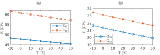
\includegraphics[width=0.95\textwidth]{Chapter_3/pztEG}
	\end{center}
	\caption{Temperature-dependent \textbf{(a)} Young's modulus (E\(_{11}\), E\(_{33}\)) and \textbf{(b)} shear modulus (G\(_{12}\), G\(_{23}\)) for the \acs{pzt}}
	\label{fig:pztEG}
\end{figure}
\begin{figure}
	\begin{center}
		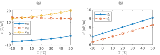
\includegraphics[width=0.95\textwidth]{Chapter_3/pztEEps}
	\end{center}
	\caption{Temperature-dependent (\textbf{a}) piezoelectric coupling coefficients (e\(_{31}\), e\(_{15}\), e\(_{33}\)) and (\textbf{b}) electric permittivity (\(\boldsymbol{\epsilon}^S_{11}\), \(\boldsymbol{\epsilon}^S_{33}\)) for the \acs{pzt}}
	\label{fig:pztEEps}
\end{figure}
\nomtypeG[\(\rho\)]{\( \rho \)}{Mass density}{}{\unit[per-mode = symbol]
	{\kilogram\per\cubic\metre}} \section{Model-assisted damage severity assessment}
\label{sec:madif}



The process of determining the damage size is shown in the flowchart in Figure \ref{fig:Flowchart} \cite{fiborek2021model}.
Before inspecting a given \ac{hsc} panel, a numerical analysis has to be performed to determine a function that describes the effect of damage on wave propagation.
Then the model is subjected to experimental validation.
If the simulation results did not agree with the measured results, the material parameters of the components were adjusted.
In the dissertation, the \ac{cfrp} volume fraction of reinforcing fibres was adjusted to determine a wave velocity \cite{kudela2007modelling} and a damping coefficient of the skin to set the magnitude of the registered signals \cite{wandowski2017guided}.
\begin{figure}[H]
	\begin{center}
		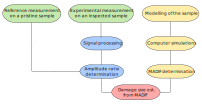
\includegraphics[width=0.95\textwidth]{Chapter_3/flowchart}
	\end{center}
	\caption{A flowchart representing the process for damage size estimation}
	\label{fig:Flowchart}
\end{figure}

When the structure model was developed, several computer simulations for various damage sizes were conducted to determine the \ac{madif}, a cornerstone of the dissertation. This function determines the severity of \ac{hsc} damage based on the signal received by the sensor.
Several excitation signals and damage indices were considered to select the best \ac{madif}.
The selection criterion was the monotonicity and the function slope over the considered range of the damage size. Then, the damage magnitude was obtained from the \ac{madif} for the measured signal and normalised to the reference one. 

\clearpage{}
\clearpage{}

\chapter{Formulation of the Time-Domain Spectral Element Method}
\label{ch:sem}
The comprehensive formulation of the \ac{sem}-based numerical model is presented in the Chapter.
It includes shape function definition, numerical integration in the scheme of the \ac{gll}, determination of the structural matrices for solid and first-order shear deformation theory elements and electromechanical coupling for the \acp{pzt}.
The non-matching interface was introduced with the novel approach based on the element shape functions.
These components were combined to implement the \ac{sem} for the honeycomb structure with the \ac{fcgm}, which has not been found in the literature before.

\section{High order polynomial interpolation and the \acl{gll} integration scheme}
\label{sec:sem}



The \ac{sem} is similar to the \ac{fem}.
The similarity of both methods lies in the fact that considered domain is divided into non-overlapping finite elements, and external forces and arbitrary boundary conditions are imposed in the particular nodes.
The main difference between those methods is a selection of the shape function \( N=N(\xi )\), pictured in Figure~\ref{fig:shape}, which is interpolated by a Lagrange polynomial that passes through the element nodes.
The nodes are localised on the endpoint of an interval, \(\xi\in[-1,1]\), and the roots of the first derivative of Legendre polynomial \(\mathcal{P}\) of degree \(p\):
\begin{eqnarray}
	(1-\xi^2)\mathcal{P}'_{p}(\xi)=0.
	\label{eq:nodes}
	\nomtypeD[x]{\( \xi, \eta, \zeta \)}{local coordinates}{}
	\nomtypeD[w]{\(w\)}{Weighting factor}{}
\end{eqnarray}
The approximation of an integral over the elements is achieved according to the \ac{gll} rule at points coinciding with the element nodes. The integration weights \(w=w(\xi)\) equal
\begin{eqnarray}
	{w(\xi)} = \frac{2}{p(p+1)(\mathcal{P}_{p}(\xi))^2}.
	\label{eq:weight}
\end{eqnarray}

The shape functions and the weights for \ac{2d} or \ac{3d} elements are obtained by the Kronecker product of vectors of individual axes, denoted by \(\otimes\) as follows:
\begin{eqnarray}
	\begin{array}{rcl}
	N(\xi,\eta) & = & N(\xi)\otimes N(\eta),\\
	N(\xi,\eta,\zeta) & = & N(\xi)\otimes N(\eta)\otimes N(\zeta),
	\end{array}
\label{eq:shape_functions}
\nomtypeD[N]{$N$}{Shape function}{}
\end{eqnarray}
\begin{eqnarray}
	\begin{array}{rcl}
	w(\xi,\eta) & = & w(\xi)\otimes w(\eta),\\
	w(\xi,\eta,\zeta) & = & w(\xi)\otimes w(\eta)\otimes w(\zeta).
	\end{array}
	\label{eq:weights}
\end{eqnarray}
\begin{figure}[H]
	\begin{center}
		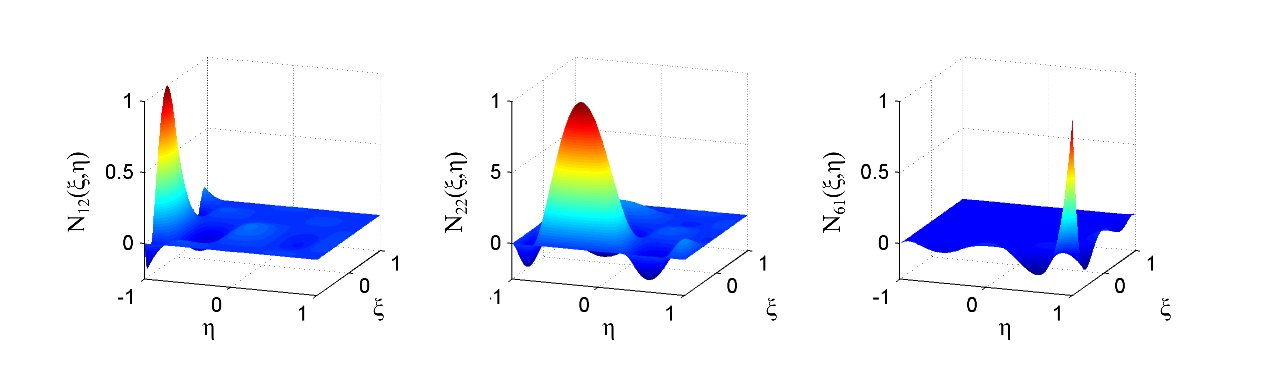
\includegraphics[width=0.95\textwidth]{Chapter_4/shape_function}
	\end{center}
	\caption{Shape functions based on fifth-order polynomial interpolation}
	\label{fig:shape}
\end{figure}

The derivation of the equation of motion is given in \cite{ostachowicz2011guided}, and it is defined as
\begin{eqnarray}
	\label{eq:motion}
	\textbf{M} \ddot{\textbf{d}} + \textbf{D} \dot{\textbf{d}} + \textbf{K} \textbf{d} = \textbf{f}_{ext},
	\nomtypeR[M]{$\textbf{M}$}{Mass matrix}{}{\unit{\kg}}\nomtypeR[D]{$\textbf{D}$}{Damping matrix}{}{\unit[per-mode = symbol]{\newton\second \per \meter}}\nomtypeR[K]{$\textbf{K}$}{Stiffness matrix}{}{\unit[per-mode = symbol]{\newton\per\metre}}\nomtypeR[force_ext]{$\textbf{f}_{ext}$}{External force vector}{}{\unit{\newton}}\nomtypeR[d]{$\textbf{d}$}{Displacements vector}{}{\unit{\meter}}\end{eqnarray}
where \textbf{d} is the displacements vector; \textbf{M}, \textbf{D} and \textbf{K} are the structural mass, damping and stiffness matrices, respectively; \textbf{F}$_{ext}$ is the external forces vector; \((\dot{\ })=\frac{\partial}{\partial t}\).
The construction of the structural matrices is similar to the classical approach in \ac{fem}.

The most significant advantage of this method is the fast convergence of the equation of motion.
It is achieved for six nodes per wavelength, while at least fifteen nodes are needed in the case of linear elements in classic \ac{fem}~\cite{wee2017simulating}.
In addition, the mass matrix is diagonal when using the \ac{gll} approach and solid elements or elements based on first-order shear deformation theory.
 \section{\Acl{2d} spectral element}
\label{sec:2Dmodel}

The shell element has five \acp{dof} at every node, three translations and two rotations as it is shown in Figure~\ref{fig:2d_se}.
All the nodes are located in the neutral surface of the element.
\begin{figure}
	\begin{center}
		\includegraphics[width=0.95\textwidth]{Chapter_4/2d_se}
	\end{center}
	\caption{\Acl{2d} spectral element}
	\label{fig:2d_se}
\end{figure}
According to the first-order shear deformation theory~\cite{reissner1945effect, mindlin1951influence}, the displacement field is expressed as
\begin{eqnarray}
	\left \{ \begin{array}{c}
		\textbf{u}^e\\
		\textbf{v}^e\\
		\textbf{w}^e
	\end{array} \right\} = 
	\left \{ \begin{array}{c}
		\textbf{u}_0^e - z\boldsymbol{\varphi}_x^e\\
		\textbf{v}_0^e - z\boldsymbol{\varphi}_y^e\\
		\textbf{w}_0^e\\
	\end{array} \right\},
\end{eqnarray}
\nomtypeR[uvw]{$u,\,v,\,w$}{Displacement in x-, y- and z-axis direction}{}{\unit{\metre}}\nomtypeG[phi]{$\varphi^e$}{Element rotation of the normal to the mid-plane}{}{\unit{\radian}}where \(\textbf{u}_0^e\), \(\textbf{v}_0^e\) and \(\textbf{w}_0^e\) are element displacements, \(\boldsymbol{\varphi}_x^e\), \(\boldsymbol{\varphi}_y^e\) are the element rotations of the normal to the mid-plane with respect to the axes \textit{x} and \textit{y}, respectively. They are defined as
\begin{eqnarray}
	\left \{\begin{array}{c}
		\textbf{u}_0^e\\
		\textbf{v}_0^e\\
		\textbf{w}_0^e\\
		\boldsymbol{\varphi}_x^e\\
		\boldsymbol{\varphi}_y^e
	\end{array} \right\}
	= \textbf{N}^e(\xi,\eta)\widehat{\textbf{d}}^e
	= \sum_{n=1}^{q+1}\sum_{m=1}^{p+1}\textbf{N}_m^e(\xi)\textbf{N}_n^e(\eta)
	\left \{ \begin{array}{c}
		\widehat{\textbf{u}}_0^e \\
		\widehat{\textbf{v}}_0^e \\
		\widehat{\textbf{w}}_0^e \\
		\widehat{\boldsymbol{\varphi}}_x^e \\
		\widehat{\boldsymbol{\varphi}}_y^e
	\end{array} \right \},
\end{eqnarray}
where \(n\) and \(m\) are the nodes number in \(\xi\) and \(\eta\) direction, respectively, \(q\) is the Legendre polynomial degree,  $\widehat{\textbf{d}}^e$ is a nodal displacements vector of the element $e$.
The element bending strain-displacement relations are given in the form
\begin{eqnarray}
	\boldsymbol{\varepsilon}_b^0 = 
	\left \{ \begin{array}{c}
		\frac{\partial \widehat{\textbf{u}}_0^e}{\partial x} \\
		\frac{\partial \widehat{\textbf{v}}_0^e}{\partial y} \\
		\frac{\partial \widehat{\textbf{u}}_0^e}{\partial y} + \frac{\partial \widehat{\textbf{v}}_0^e}{\partial x}\\
		\frac{\partial \widehat{\boldsymbol{\varphi}}_x^e}{\partial x} \\
		\frac{\partial \widehat{\boldsymbol{\varphi}}_y^e}{\partial y} \\
		\frac{\partial \widehat{\boldsymbol{\varphi}}_x^e}{\partial y} + \frac{\partial \widehat{\boldsymbol{\varphi}}_y^e}{\partial x}
	\end{array} \right\} = 
	\textbf{B}_b^e\widehat{\textbf{d}}^e = 
	\left [
	\begin{array}{ccccc}
		\frac{\partial N^e}{\partial x} & 0 & 0 & 0 & 0\\
		0 & \frac{\partial N^e}{\partial y} & 0 & 0 & 0\\
		\frac{\partial N^e}{\partial y} & \frac{\partial N^e}{\partial x} & 0 & 0 & 0\\
		0 & 0 & 0 & -\frac{\partial N^e}{\partial x} & 0\\
		0 & 0 & 0 & 0 & -\frac{\partial N^e}{\partial y}\\
		0 & 0 & 0 & -\frac{\partial N^e}{\partial y} & -\frac{\partial N^e}{\partial x}
	\end{array} \right]
	\left \{ \begin{array}{c}
		\widehat{\textbf{u}}_0^e \\
		\widehat{\textbf{v}}_0^e \\
		\widehat{\textbf{w}}_0^e \\
		\widehat{\boldsymbol{\varphi}}_x^e \\
		\widehat{\boldsymbol{\varphi}}_y^e
	\end{array} \right\}.
\end{eqnarray}
The element shear strain--displacement relations are given in the form
\begin{eqnarray}
	\boldsymbol{\varepsilon}_s^e = 
	\left \{ \begin{array}{c}
		\frac{\partial \widehat{\textbf{w}}_0^e}{\partial x} + \widehat{\boldsymbol{\varphi}}_x^e\\
		\frac{\partial \widehat{\textbf{w}}_0^e}{\partial y} + \widehat{\boldsymbol{\varphi}}_y^e
	\end{array} \right\} = 
	\textbf{B}_s^e\widehat{\textbf{d}}^e = 
	\left [
	\begin{array}{ccccc}
		0 & 0 & \frac{\partial N^e}{\partial y} & -N^e & 0\\
		0 & 0 & \frac{\partial N^e}{\partial y} & 0 & -N^e
	\end{array} \right]
	\left \{ \begin{array}{c}
		\widehat{\textbf{u}}_0^e \\
		\widehat{\textbf{v}}_0^e \\
		\widehat{\textbf{w}}_0^e \\
		\widehat{\boldsymbol{\varphi}}_x^e \\
		\widehat{\boldsymbol{\varphi}}_y^e
	\end{array} \right\}.
\end{eqnarray}
\nomtypeD[Eps]{$\boldsymbol{\varepsilon}$}{Strain tensor}{}The mass and stiffness matrices for \ac{2d} elements are defined as:
\begin{eqnarray}
	\textbf{M}_{dd}^e & = &
	\left [
	\begin{array}{cc}
		\textbf{M}^e & 0\\
		0 & \textbf{J}^e
	\end{array}
	\right] =
	\int_{\Omega^e}\textbf{N}^{\mathrm{T}}\rho
	\left [
	\begin{array}{ccccc}
		h^e & 0 & 0 & 0 & 0 \\
		& h^e & 0 & 0 & 0 \\
		&  & h^e & 0 & 0\\
		&  &  & \frac{{h^e}^3}{12} & 0\\
		Sym. &  &  &  & \frac{{h^e}^3}{12}
	\end{array} \right]
	\textbf{N} \diff\Omega^e,\\
	\textbf{K}_{dd}^e & = & \int_{\Omega^e}{\textbf{B}_b^e}^{\mathrm{T}}
	\left[
	\begin{array}{cc}
		\check{\textbf{A}} & \check{\textbf{B}}\\
		\check{\textbf{B}} & \check{\textbf{D}}
	\end{array} \right]
	\textbf{B}_b^e \diff \Omega^e+\int_{\Omega^e}{\textbf{B}_s^e}^{\mathrm{T}}\hat{\textbf{A}}\textbf{B}_s^e\diff \Omega^e,
\end{eqnarray}
\nomtypeR[B]{$\textbf{B}$}{Strain-displacement matrix}{}{\unit{\per\meter}}\nomtypeR[he]{$h^e$}{Element thickness}{}{\unit{\meter}}\nomtypeG[Omega]{$\Omega^e$}{Element area}{}{\unit{\square\meter}}where \(h^e=h_t+h_b\) is the element thickness, while \(h_{t(b)}\) is the distance between mid-plane and top (bottom) surface of the element, and \(\Omega_e\) is the element area.
The superscript T denotes a transpose matrix.
The sub-matrices \(\check{\textbf{A}},\,\hat{\textbf{A}},\,\check{\textbf{B}}\,\mathrm{and}\,\check{\textbf{D}}\) are defined as
\begin{eqnarray}
	\check{\textbf{A}} & = & \textbf{c}_{ij}\,(h_t-h_b),\qquad i,j=1,2,6\nonumber,\\
	\check{\textbf{B}} & = & \textbf{c}_{ij}\,(h_t^2-h_b^2)/2,\qquad i,j=1,2,6\nonumber,\\
	\check{\textbf{D}} & = & \textbf{c}_{ij}\,(h_t^3-h_b^3)/3,\qquad i,j=1,2,6\nonumber,\\
	\hat{\textbf{A}} & = & 5/4\,\textbf{c}_{ij}\,\left[h_t-h_b-4/3\left(h_t^3-h_b^3\right)/{h^e}^2\right],\qquad i,j=4,5.
\end{eqnarray}
\nomtypeR[c]{$\textbf{c}$}{Elasticity tensor}{}{\unit[per-mode = symbol]{\newton\per\square\meter}}% \section{\Acl{3d} spectral element}
\label{sec:3Dmodel}

The solid element has three mechanical \acp{dof} per node, as it is shown in Figure~\ref{fig:3d_se}.
\begin{figure}
	\begin{center}
		\includegraphics[width=0.95\textwidth]{Chapter_4/3d_se}
	\end{center}
	\caption{\Acl{3d} spectral element}
	\label{fig:3d_se}
\end{figure}
The displacement vector of the element based on \ac{3d} elasticity of solids is composed of three translations defined as
\begin{eqnarray}
	\left \{ \begin{array}{c}
		\textbf{u}^e\\
		\textbf{v}^e\\
		\textbf{w}^e
	\end{array} \right\} = \textbf{N}^e(\xi,\eta, \zeta)\widehat{\textbf{d}}^e = \sum_{l=1}^{r+1}\sum_{n=1}^{q+1}\sum_{m=1}^{p+1}\textbf{N}_m^e(\xi)\textbf{N}_n^e(\eta)\textbf{N}_l^e(\zeta)
	\left \{ \begin{array}{c}
		\widehat{\textbf{u}}^e\\
		\widehat{\textbf{v}}^e\\
		\widehat{\textbf{w}}^e
	\end{array} \right\},
	\label{eq:3D_displ}
\end{eqnarray}
where \(l\) is the nodes number in \(\zeta\) direction, \(r\) is the Legendre polynomial degree, \(\widehat{\textbf{u}}^e\), \(\widehat{\textbf{v}}^e\) and 
\(\widehat{\textbf{w}}^e\) are displacements of the element nodes in \(\xi,\eta\) and \(\zeta\) direction.

The nodal strain--displacement relations implemented bu Kudela et al. \cite{kudela20093d} are given as
\begin{eqnarray}
	\boldsymbol{\varepsilon}^e = 
	\left \{ \begin{array}{c}
		\frac{\partial \widehat{\textbf{u}}^e}{\partial x} \\
		\frac{\partial \widehat{\textbf{v}}^e}{\partial y} \\
		\frac{\partial \widehat{\textbf{w}}^e}{\partial z} \\
		\frac{\partial \widehat{\textbf{v}}^e}{\partial z} + \frac{\partial \widehat{\textbf{w}}^e}{\partial y}\\
		\frac{\partial \widehat{\textbf{u}}^e}{\partial z} + \frac{\partial \widehat{\textbf{w}}^e}{\partial x}\\
		\frac{\partial \widehat{\textbf{v}}^e}{\partial y} + \frac{\partial \widehat{\textbf{v}}^e}{\partial x}
	\end{array} \right\} = \textbf{B}^e\widehat{\textbf{d}}^e =
	\left [
	\begin{array}{ccc}
		\frac{\partial N^e}{\partial x} & 0 & 0\\
		0 & \frac{\partial N^e}{\partial y} & 0\\
		0 & 0 & \frac{\partial N^e}{\partial z}\\
		0 & \frac{\partial N^e}{\partial z} & \frac{\partial N^e}{\partial y}\\
		\frac{\partial N^e}{\partial z} & 0 & \frac{\partial N^e}{\partial x}\\
		\frac{\partial N^e}{\partial y} & \frac{\partial N^e}{\partial x} & 0
	\end{array} \right]
	\left \{ \begin{array}{c}
		\widehat{\textbf{u}}^e \\
		\widehat{\textbf{v}}^e \\
		\widehat{\textbf{w}}^e
	\end{array} \right\}.
\end{eqnarray}
The formulae of the structural matrices for \ac{3d} elements are
\begin{eqnarray}
	\textbf{M}_{dd}^e & = & \int_{V^e}\textbf{N}^{\mathrm{T}}\rho \textbf{N} \diff V^e,\\
	\textbf{K}_{dd}^e & = & \int_{V^e}{\textbf{B}_d^e}^{\mathrm{T}}\textbf{c}\textbf{B}_d^e \diff V^e,
\end{eqnarray}
\nomtypeR[Ve]{$V^e$}{Element volume}{}{\unit{\cubic\meter}}where \textbf{c} is the elasticity tensor, \(\rho\) is mass density, and \(V_e\) is the element volume. \section{The \acl{pzt} modelling}
\label{sec:PZTmodel}

The electromechanical coupling is governed by the linear constitutive equation of piezoelectric material according to~\cite{giurgiutiu2009micromechatronics, rekatsinas2017cubic}, and this is defined as
\begin{eqnarray}
	\left [ 
	\begin {array}{c}
	\boldsymbol{\sigma}\\
	\widetilde{\textbf{D}}
\end{array}\right ]=
\left [ 
\begin{array}{cc}
	\textbf{c}^E & -\textbf{e}^{\mathrm{T}} \\
	\textbf{e} & \epsilon^S 
\end{array} \right ]
\left[ 
\begin{array}{c}
	\boldsymbol{\varepsilon}\\
	\widetilde{\textbf{E}} 
\end{array} \right ],
\label{eq:elecmechcoupling}
\end{eqnarray}
\nomtypeR[Ep]{$\widetilde{\textbf{E}} $}{Electric field}{}{\unit[per-mode=symbol]{\newton\per\coulomb}}\nomtypeR[Dp]{$\widetilde{\textbf{D}} $}{Electric charge density displacement}{}{\unit[per-mode=symbol]{\coulomb\per\square\metre}}\nomtypeG[phip]{$\boldsymbol{\phi}$}{Electric potential vector}{}{\unit{\volt}}\nomtypeG[sigma]{$\boldsymbol{\sigma}$}{Stress tensor}{}{\unit [per-mode = symbol]{\newton \per \square \meter }}where \(\boldsymbol{\sigma}\) is the stress components, \(\textbf{c}^E\) is the stiffness coefficient matrix measured at zero electric field, \textbf{e} is the piezoelectric coupling tensor, \(\boldsymbol{\epsilon}^S\) is the electric permittivity measured at zero strain, and \(\widetilde{\textbf{E}}\) and \(\widetilde{\textbf{D}}\) are the electric field and electric charge density displacement.
The electric field of the element is defined as
\begin{eqnarray}
\widetilde{\textbf{E}}^e=-\textbf{B}_\phi^e \widehat{\boldsymbol{\phi}}^e = \left[ \begin{array}{c}
	\frac{\partial N^e}{\partial \xi}\\
	\frac{\partial N^e}{\partial \eta}\\
	\frac{\partial N^e}{\partial \zeta}
\end{array} \right] \widehat{\boldsymbol{\phi}}^e,
\end{eqnarray}
where \(\widehat{\boldsymbol{\phi}}^e\) is a nodal voltage of the transducer. The \ac{sem} formulation of the governing equation (\ref{eq:elecmechcoupling}) is defined as:
\begin{eqnarray}
	\left [\begin{array}{cc}
		\textbf{M}_{dd} & \textbf{0}\\
		\textbf{0} & \textbf{0}
	\end{array}\right]
	\left \{\begin{array}{c}
		\widehat{\ddot{\textbf{d}}} \\
		\textbf{0}
	\end{array}\right \} +
	\left [\begin{array}{cc}
		\textbf{K}_{dd} & \textbf{K}_{d \phi}\\
		\textbf{K}_{d \phi}^{\mathrm{T}} & \textbf{K}_{\phi \phi}
	\end{array}\right]
	\left \{\begin{array}{c}
		\widehat{\textbf{d}} \\
		\widehat{\boldsymbol{\phi}}
	\end{array}\right \}  = 
	\left \{\begin{array}{c}
		\textbf{0}\\
		\widehat{\textbf{Q}}
	\end{array}\right \},
	\label{eq:pzt_sem}
\end{eqnarray}
\nomtypeR[Q]{$\textbf{Q}$}{Charge vector}{}{\unit{\coulomb}}where \(\widehat{\textbf{Q}}\) is the nodal charge vector.
The mass and stiffness matrices are defined according to \ac{3d} model from Section \ref{sec:3Dmodel}.
The piezoelectric coupling matrix \(\textbf{K}_{\phi \phi}^e\) and the dielectric permittivity matrix \(\textbf{K}_{d \phi}^e\) are defined as
\begin{eqnarray}
	\textbf{K}_{d\phi}^e & = & \int_{V_e}{\textbf{B}_d^e}^{\mathrm{T}}\textbf{e}^{\mathrm{T}} \textbf{B}_{\phi}^e \diff V_e,\\
	\textbf{K}_{\phi \phi}^e & = & -\int_{V_e}{\textbf{B}_{\phi}^e}^{\mathrm{T}} 
	{\textbf{\(\epsilon\)}^S}^{\mathrm{T}} \textbf{B}_{\phi}^e \diff V_e.
\end{eqnarray}

If a vector \(\textbf{b}\) contains list of consecutive boundary nodes (corresponding to electrodes) and a vector \(\textbf{a}\) contains lists of consecutive active nodes (remaining nodes) of the \ac{pzt}, the electrical potential vector and the charge vector can be rewritten as:
\begin{eqnarray}
	\widehat{\boldsymbol{\phi}} & = & \left \{\begin{array}{cc}
		\widehat{\boldsymbol{\phi}}(\textbf{b}) &
		\widehat{\boldsymbol{\phi}}(\textbf{a})
	\end{array}\right \}^{\mathrm{T}},\\
	\widehat{\textbf{Q}} & = & \left \{\begin{array}{cc}
		\widehat{\textbf{Q}}(\textbf{b}) & \textbf{0}
	\end{array}\right \}^{\mathrm{T}}.
	\label{eq:phi_Q}
\end{eqnarray}
Then, piezoelectric part of Eq.~(\ref{eq:pzt_sem}) is expressed as
\begin{eqnarray}
	\begin{split}
		\left [\begin{array}{cc}
			\textbf{K}_{d \phi}(:,\textbf{b}) &
			\textbf{K}_{d \phi}(:,\textbf{a})
		\end{array}\right]^{\mathrm{T}}
		\widehat{\textbf{d}} & +
		\left [\begin{array}{cc}
			\textbf{K}_{\phi \phi}(\textbf{b},\textbf{b}) & \textbf{K}_{\phi 		\phi}(\textbf{b},\textbf{a})\\
			\textbf{K}_{\phi \phi}(\textbf{a},\textbf{b}) & \textbf{K}_{\phi \phi}(\textbf{a},\textbf{a})
		\end{array}\right]
		\left \{\begin{array}{c}
			\widehat{\boldsymbol{\phi}}(\textbf{b}) \\
			\widehat{\boldsymbol{\phi}}(\textbf{a})
		\end{array}\right \}\\ 
		& = \left \{\begin{array}{c}
			\widehat{\textbf{Q}}(\textbf{b}) \\
			\textbf{0}
		\end{array}\right \},
	\end{split}
	\label{eq:pztboundary}
\end{eqnarray}
where the notation \(\textbf{K}(\textbf{r},\textbf{c})\) uses vectors \(\textbf{r}\) and \(\textbf{c}\) to extract rows and columns from the matrix \(\textbf{K}\), respectively, and \((:)\) means all rows or columns of \(\textbf{K}\).
The electrical potential of the free nodes can be extracted from Eq.~(\ref{eq:pztboundary}) in the form
\begin{eqnarray}
	\widehat{\boldsymbol{\phi}}(\textbf{a}) = -\textbf{K}_{\phi\phi}^{-1}(\textbf{a},\textbf{a})\left[\textbf{K}_{\phi d}(\textbf{a},:) \widehat{\textbf{d}} + \textbf{K}_{\phi\phi}(\textbf{a},\textbf{b})\widehat{\boldsymbol{\phi}}(\textbf{b}) \right].
	\label{eq:freePotetial}
\end{eqnarray}
If the \ac{pzt} acts as an actuator, the electrical potential of the electrode nodes has the values of the applied signal.
As one of the electrodes is grounded, the potential is zero.
Therefore, the potential vector can be written as
\begin{eqnarray}
	\widehat{\boldsymbol{\phi}}(\textbf{b}) = \left \{\begin{array}{cc}
		\widehat{\boldsymbol{\phi}}(\textbf{b}_v) &
		\widehat{\boldsymbol{\phi}}(\textbf{b}_g)
	\end{array}\right \}^{\mathrm{T}}=\left \{\begin{array}{cc}
	\textbf{V}(t) & \textbf{0}
	\end{array}\right \}^{\mathrm{T}},
	\label{eq:phi_V}
\end{eqnarray}
where \(\textbf{b}_v\) is a list of nodes of the applied electrode and \(\textbf{b}_g\) is a list of nodes of the grounded electrode and \(\textbf{V}(t)\) is the applied voltage signal.
Substituting Eq. (\ref{eq:phi_V}) into Eq. (\ref{eq:freePotetial}) and Eq. (\ref{eq:pztboundary}), induced stiffness of the actuator is obtained as
\begin{eqnarray}
	\textbf{K}_{a}=-\textbf{K}_{d\phi}(:,\textbf{a})\,\textbf{K}_{\phi \phi}^{-1}(\textbf{a},\textbf{a})\,\textbf{K}_{\phi \phi} (\textbf{a},\textbf{b}).
\end{eqnarray}
Hence, the equivalent mechanical force vector of the applied voltage of the piezoelectric actuator equals
\begin{eqnarray}
	\widehat{\textbf{f}}_{a}=-\textbf{K}_{a}\,\widehat{\boldsymbol{\phi}}(\textbf{b}).
	\label{eq:f_act}
\end{eqnarray}
\nomtypeR[force_act]{$\textbf{f}_{a}$}{Actuator equivalent force vector}{}{\unit{\newton}}In the case of the open circuit sensor one electrode is grounded so the electric potential of the free nodes becomes as
\begin{eqnarray}
	\widehat{\boldsymbol{\phi}}(\textbf{a}) = -\textbf{K}_{\phi\phi}^{-1}(\textbf{a},\textbf{a})\,\textbf{K}_{\phi d}(\textbf{a},:)\,\widehat{\textbf{d}}.
	\label{eq:sensorPotetial}
\end{eqnarray}
The induced stiffness of the sensor can be written as
\begin{eqnarray} \textbf{K}_s=\textbf{K}_{d \phi}(:,\textbf{a})\,\textbf{K}_{\phi \phi}^{-1} (\textbf{a},\textbf{a})\,\textbf{K}_{\phi d}(\textbf{a},:).
\end{eqnarray}
To obtain the sensor response, the nodal electric potential must be integrated over the electrode surface as follows
\begin{eqnarray}
	\boldsymbol{\phi}(t) = \int_{\Omega_s}\widehat{\phi} \diff\Omega_s.
	\label{eq:sensorResponse}
\end{eqnarray} \section{Structural damping}
\label{sec:damping}

Propagating waves in the structure attenuate due to many factors, including geometric spreading, material damping, and dissipation into the adjacent domain.
This study adopted the Rayleigh damping model for the \ac{cfrp} skin and adhesive layer, while the damping for the aluminium core and the \ac{pzt} was neglected.
According to \cite{wandowski2017guided}, the Rayleigh damping model is defined as
\begin{eqnarray}
	\textbf{D}_{dd}^e = \alpha_M \textbf{M}_{dd}^e + \beta_K \textbf{K}_{dd}^e,
	\label{eq:damping}
\end{eqnarray}
\nomtypeD[alpha]{$\alpha_M$}{Mass-proportionality damping coefficient}{}\nomtypeD[beta]{$\beta_K$}{Stiffness-proportionality damping coefficient}{}where \(\alpha_M\) and \(\beta_K\) are the mass- and stiffness- proportionality coefficients.
In the presented model, \(\beta_K\) was assumed to be zero to ensure that matrix \(\textbf{D}_{dd}\) remains diagonal \cite{schulte2011simulation, wandowski2017guided}.
This assumption gives a good approximation when considering a single mode and a specific frequency. 
Ramadas showed slight differences in Lamb wave attenuation by analysing three models, i.e. mass-, stiffness-proportional and the sum of both \cite{ramadas2011modelling}.
However, due to the diagonal damping matrix, the mass-proportional model is computationally more efficient than the other models. \section{Displacements coupling at the interface of substructures}
\label{sec:interface}

The proposed model of the sandwich panel consisted of \ac{2d} and \ac{3d} elements.
In the combination of such elements, there are no common nodes because the nodes of the shell element are localised on the mid-plane of the component.
I realised the connection of both elements in a paper regarding the research on the effect of the glue thickness between the \ac{pzt} and the host plate on the propagation of elastic waves in a composite plate \cite{fiborek20192d}.
Connection was made possible by incorporating interface elements between both components.
The interface was implemented based on Lagrange multipliers, which are interpreted as forces imposed to determine the appropriate displacements of nodes. My approach was similar to the interface for two shell elements proposed by Ashawin et al. \cite{ashwin2014formulation}.
To avoid creating coincided meshes for all components of \ac{hsc}, a non-matching interface should be used.
For this purpose, I proposed a novel approach for Lagrange multipliers-based interface, which creates a coupling matrix by the spectral elements shape function.
The non-matching interface was incorporated in the simulations of \ac{gw} registered by the \ac{fbg} sensor \cite{fiborek2022spectral}.
This paper is an original work regarding modelling such a sensor by the \ac{sem} \cite{fiborek2022spectral}.

\begin{figure}[!htb]
	\begin{center}
		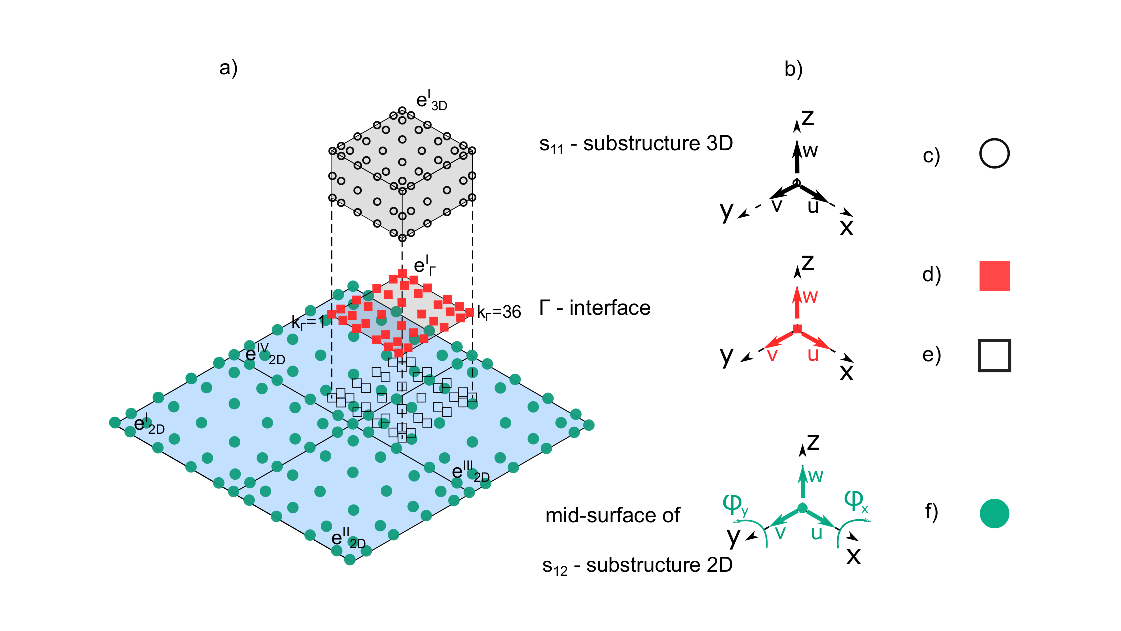
\includegraphics[width=1\textwidth]{Chapter_4/interface_2D3D}
	\end{center}
	\caption{Non-matching interface setup: (\textbf{a}) interface coupling, (\textbf{b}) the interface and the substructures degrees-of-freedom}
	\label{fig:interface}
\end{figure}
The non-matching interface between \ac{2d} and \ac{3d} elements is presented in Figure~\ref{fig:interface}.
The coupling of two domains imposes zero displacements relative to each other.
It can be expressed as
\begin{eqnarray}
	\left\{\begin{array}{c}
		\textbf{u}\\
		\textbf{v}\\
		\textbf{w}
	\end{array}\right\}_{s_{i1}}^{\Gamma^i}-
	\left\{\begin{array}{c}
		\textbf{u}\\
		\textbf{v}\\
		\textbf{w}
	\end{array}\right\}_{s_{i2}}^{\Gamma^i}=
	\left\{\begin{array}{c}
		\textbf{0}\\
		\textbf{0}\\
		\textbf{0}
	\end{array}\right\},
	\label{eq:coupling}
	\nomtypeD[Gamma]{$\Gamma$}{Interface}{}
\end{eqnarray}
where \(s_{i1}\) and \(s_{i2}\) are components connected by the interface \(\Gamma^i\).
For the whole structure, the Eq.~(\ref{eq:coupling}) can be written in the matrix form
\begin{eqnarray}
	\textbf{G}\textbf{d}=\textbf{0},
	\label{eq:cond_disp}
	\nomtypeD[G]{$\textbf{G}$}{Interface coupling matrix}{}
\end{eqnarray}
where \textbf{G} is the coupling matrix which contains the equations to interpolate the substructures displacements at the interfaces, and \(\textbf{d}\) is a global displacement field for \(nS\) number of substructures, composed as
\begin{eqnarray}
	\textbf{d} = \left\{\begin{array}{cccc}
		\textbf{d}_1, & \textbf{d}_2, &\ldots, & \textbf{d}_{nS}
	\end{array}\right\}^T.
	\label{eq:displacements}
\end{eqnarray}

\begin{algorithm}
	\SetAlgoLined
	\For{i = 1 \KwTo 2}{
		create \(n^{\Gamma}\times n^{s_i}\) null matrix 
		\(\mathbf{G}_i\),\\
		\For{j = 1 \KwTo \(n^{\Gamma}\)} {
			find \(ownerElement^j_i\) in the structure \(s_i\) 
			containing interface node \(j\) with global coordinates vector: 
			\(X_p=(x^j_p,y^j_p)\)\;
			assign vector \(X_e=(x_e,y_e)\) of coordinates of all nodes in 
			\(ownerElement^j_i\)\,
			assign initial coordinates 
			\(X_{\kappa}=(x^j_{\kappa},y^j_{\kappa})\) to the nearest node in
			\(ownerElement^j_i\) to node \(j\)\,
			transform global coordinates \(X_{\kappa}\) to a local coordinate system \(\xi_{\kappa}=\xi(X_{\kappa});\quad 
			\eta_{\kappa}=\eta(X_{\kappa})\)\,
			\While{\(\left|X_p-X_{\kappa}\right|>\mathrm{tol}\)}{
				\(\xi_{\kappa+1}=\xi_{\kappa}+(\mathcal{J}_{\kappa})^{1,1}_{\mathrm{inv}}(x^j_p-x_{\kappa}^j)
				+(\mathcal{J}_{\kappa})^{1,2}_{\mathrm{inv}}(y^j_p-y_{\kappa}^j)\)\,
				\(\eta_{\kappa+1}=\eta_{\kappa}+(\mathcal{J}_{\kappa})^{2,1}_{\mathrm{inv}}(x^j_p-x_{\kappa}^j)
				+(\mathcal{J}_{\kappa})^{2,2}_{\mathrm{inv}}(y^j_p-y_{\kappa}^j)\)\,
				\(X_{\kappa}=N_{\kappa+1}X_e\)\,
			}
			\(\mathbf{G}_i(j,n^{X_e})=N_{\kappa+1}\)\,
		}
		\uIf{\(s_i\) \(\mathrm{is\ 3D}\)} {
			\(\mathbf{G}_i=\left[\begin{array}{ccc}
				\mathbf{G}_i & \mathbf{0} & \mathbf{0}\\
				\mathbf{0} & \mathbf{G}_i & \mathbf{0}\\
				\mathbf{0} & \mathbf{0} & \mathbf{G}_i
			\end{array} \right]
			\)\,
		}
		\ElseIf{\(s_i\) \(\mathrm{is\ 2D}\)} {
			\(\mathbf{G}_i=\left[\begin{array}{ccccc}
				\mathbf{G}_i & \mathbf{0} & \mathbf{0} & 
				\frac{h_i}{2}\mathbf{G}_i & \mathbf{0}\\
				\mathbf{0} & \mathbf{G}_i & \mathbf{0} & \mathbf{0} & 
				\frac{h_i}{2}\mathbf{G}_i\\
				\mathbf{0} & \mathbf{0} & \mathbf{G}_i & \mathbf{0} & 
				\mathbf{0}
			\end{array} \right]\)\,
		}
	}
	\KwResult{coupling matrix \(\mathbf{G}=\left[\begin{array}{cc}
		\mathbf{G}_1 & \mathbf{G}_2
	\end{array} \right],\)}
	where \(s_i\) is one of the coupled structures,\\
	\(n^{\Gamma}\) and \(n^{s_i}\) are node numbers of the interface and node numbers of the structure \(s_i\), respectively,\\ \(\left(\mathcal{J}_{\kappa}\right)_{\mathrm{inv}}\) is the inverse Jacobian matrix evaluated at \((\xi_{\kappa},\eta_{\kappa})\),\\
	\(N_{\kappa+1}\) is the shape function evaluated at \((\xi_{\kappa+1},\eta_{\kappa+1})\),\\
	\(n^{X_e}\) is the vector of global order numbers of all nodes in the \(ownerElement^j_i\)\\
	\(h_i\) is a thickness of the structure \(s_i\) and \(tol\) is a termination criterion for iterations.
	\caption{Interface coupling matrix formulation}
	\label{alg:G_matrix}
	\nomtypeD[Jacobian]{$\mathcal{J}$}{Jacobian matrix}{}\nomtypeD[nmn]{$n,m,n$}{Nodes numbers}{}\nomtypeR[Xp]{$X_p$}{Coordinates vector of the interface point}{}{\unit{\metre}}\nomtypeR[Xe]{$X_e$}{Coordinates vector of the element nodes}{}{\unit{\metre}}\end{algorithm}
General formulation of the matrix \textbf{G} is presented in Algorithm \ref{alg:G_matrix}.
The main task in this procedure is to calculate shape functions for each adjacent substructure at the points \(X_p=(x_p^k,y_p^k)\), which are projections of the interface nodes onto these substructures.
The shape function can be calculated after finding an owner element and local coordinates of the points.
Owner element is a spectral element in the domain of the substructure \(s_{ij}\) which contains interface node, for example, interface node \(k_\Gamma=36\) shown in~Figure~\ref{fig:interface}(\textbf{a}) is located in the element \(e^{I}_{3\mathrm{D}}\) and \(e^{III}_{2\mathrm{D}}\) for the substructures \(s_{11}\) and \(s_{12}\), respectively.
It can be found in two ways: using Matlab's built-in function \verb+inpolygon+ or more efficient procedure proposed by Silva et al. \cite{silva2009exact} which was used in the current implementation.\\
\\
In this procedure, an initial approximation was first performed by rejecting all external points outside the rectangular region bounded by the points \(\mathrm{P_{min}}\) and \(\mathrm{P_{max}}\) as shown in Figure \ref{fig:b_b_test}(\textbf{a}).
If \(\mathrm{X_p}\) is inside the element, then the vectors \(\vec{V}_1\) and \(\vec{V}_2\) have the same direction.
\(\vec{V}_1\) and \(\vec{V}_2\) are defined as
\begin{eqnarray}
	\vec{V}_1 & = & \vec{v}_1\times \vec{v}_p,\\
	\vec{V}_2 & = & \vec{v}_p\times \vec{v}_2.
\label{eq:v_vectors}
\nomtypeD[vvv]{$\vec{v}_p,\,\vec{v}_1,\,\vec{v}_2$}{Cross-product test  vectors}{}\nomtypeD[V1]{$\vec{V_1}$}{First cross-product vector}{}\nomtypeD[V2]{$\vec{V_2}$}{Second cross-product vector}{}\end{eqnarray}
The vectors \(\vec{v}_p\), \(\vec{v_1}\) and \(\vec{v_2}\) are pictured in Figure \ref{fig:b_b_test}(\textbf{b}). \(\vec{V}_1\) and \(\vec{V}_2\) have the same direction if the inequality \(\vec{V}_1 \cdot \vec{V}_2 \geq0\) is satisfied for each element vertex \(i\).
Then, the transformation from global to local coordinates was realised by the iterative method presented in the work of Li et al.~\cite{li2014efficient} (see also \verb+while-loop+ in Algorithm~\ref{alg:G_matrix}).
\begin{figure}[H]
	\begin{center}
		\includegraphics[width=0.95\textwidth]{Chapter_4/b_b_test}
	\end{center}
	\caption{Owner element for Xp interface node (\textbf{a}) boundary test, (\textbf{b}) cross-product test}
	\label{fig:b_b_test}
\end{figure}
While the cross-product test was exact for elements with linear edges, the approximation of the boundary test was used for second order elements, and then \(\xi_{\kappa}\) and \(\eta_{\kappa}\) must satisfy the condition \(-1\leq \xi_{\kappa},\eta_{\kappa} \leq 1\).

The computational effectiveness of Algorithm~\ref{alg:G_matrix} can be easily improved if certain precautions are taken.
Firstly, the mesh of the interface has to be based on the mesh from one of the substructures \(s_{i}\), which may be referred to as a slave.
Shape functions evaluated at (\(\xi\), \(\eta\)) may take only zero and one values.
Moreover, the code was vectorised rather than using a for-loop form, provided that the required matrix of size \(4n^e\times n^{\Gamma}\), where \(n^e\) is the number of elements of the structure \(s_i\) elements, does not exceed the operating memory. \section{Transformation of the core elements}
\label{sec:transformation}

All core elements are rotated relative to both skins, and thus it is necessary to transform the degrees of freedom from the local coordinate system of the core to the global coordinate system.
For this purpose, an additional sixth \ac{dof} was incorporated, i.e., rotation with respect to the \textit{z}-axis:
\begin{eqnarray}
	\widehat{\textbf{d}}^e_g = \left \{\begin{array}{cccccc}
		\widehat{\textbf{u}}^e & \widehat{\textbf{v}}^e &
		\widehat{\textbf{w}}^e & \widehat{\boldsymbol{\varphi}}_x^e &
		\widehat{\boldsymbol{\varphi}}_y^e & \widehat{\boldsymbol{\varphi}}_z^e
	\end{array}\right \}^{\mathrm{T}}_g.
	\label{eq:d6}
\end{eqnarray}

First, the displacement vector was transformed from the global to local coordinate system by the direction cosines as follows
\begin{eqnarray}
	\widehat{\textbf{d}}^e_l = \left \{\begin{array}{c}
		\widehat{\textbf{u}}^e \\ \widehat{\textbf{v}}^e \\
		\widehat{\textbf{w}}^e \\ \widehat{\boldsymbol{\varphi}}_x^e \\
		\widehat{\boldsymbol{\varphi}}_y^e
	\end{array}\right \}_l = 
	\left [\begin{array}{ccccc}
		\mathcal{V}^e_1, & \mathcal{V}^e_2, & \mathcal{V}^e_3, & \textbf{0} & \textbf{0} \\
		\textbf{0} & \textbf{0} & \textbf{0} & \mathcal{V}^e_1, & \mathcal{V}^e_2
	\end{array}\right ]^{\mathrm{T}}
	\left \{\begin{array}{c}
		\widehat{\textbf{u}}^e \\ \widehat{\textbf{v}}^e \\
		\widehat{\textbf{w}}^e \\ \widehat{\boldsymbol{\varphi}}_x^e \\
		\widehat{\boldsymbol{\varphi}}_y^e\\
		\widehat{\boldsymbol{\varphi}}_z^e
	\end{array}\right \}_g,
	\label{eq:d_local}
\end{eqnarray}
\nomtypeD[vector_cos]{\(\mathcal{V}^e_1,\,\mathcal{V}^e_2,\,\mathcal{V}^e_3\)}{Direction cosines}{}where \(g\) and \(l\) mean global and local coordinate system, respectively, \(\mathcal{V}^e_1\),\(\mathcal{V}^e_2\) and \(\mathcal{V}^e_3\) are direction cosines of the core element.
Then, internal forces were calculated according to guideline from Section \ref{sec:gpu} and transformed to a global coordinate system by the direction cosines as
\begin{eqnarray}
	\left\{\textbf{F}_{int}\right\}^e_g =
	\left [\begin{array}{ccccc}
		\mathcal{V}^e_1, & \mathcal{V}^e_2, & \mathcal{V}^e_3, & \textbf{0} & \textbf{0} \\
		\textbf{0} & \textbf{0} & \textbf{0} & \mathcal{V}^e_1, & \mathcal{V}^e_2
	\end{array}\right ]
	\left \{\begin{array}{c}
		\textbf{F}^1_{int} \\
		\textbf{F}^2_{int} \\
		\textbf{F}^3_{int} \\
		\textbf{F}^4_{int} \\
		\textbf{F}^5_{int} \\
	\end{array}\right \}_l^e.
	\label{eq:f_global}
\end{eqnarray}

Additionally, a part of the mass matrix accounted for rotational inertia was transformed, and, in contrast to the vector of internal forces, it had to be done only once in pre-processing as follows:

\begin{eqnarray}
	\textbf{J}_g=\left [ 
	\begin{array}{ccc}
		\left (\textbf{J}\right)^{1,1}_g & \left (\textbf{J}\right )^{1,2}_g & \left (\textbf{J}\right )^{1,3}_g\\
		& \left (\textbf{J}\right )^{2,2}_g & \left (\textbf{J}\right )^{2,3}_g\\
		Sym. &  & \left (\textbf{J}\right )^{3,3}_g\\
	\end{array}
	\right ]
	=\left[\begin{array}{ccc}
		\mathcal{V}_1, \mathcal{V}_2, \mathcal{V}_3 \end{array}\right ]^{\mathrm{T}}
	\,\textbf{J}_l\,
	\left[\begin{array}{ccc}
		\mathcal{V}_1, \mathcal{V}_2, \mathcal{V}_3 \end{array}\right ].
	\label{eq:inertia}
\end{eqnarray}
\nomtypeR[inertia]{$\textbf{J}$}{Mass moment of inertia matrix}{}{\unit{\kg\cubic\metre}}As the transfered matrix is non-diagonal, some approximation is necessary.
Surana analysed a lumped mass matrix with non-zero inertia for shell elements \cite{surana1980transition}.
He presented several formulations for a transformed mass matrix to zero off-diagonal values without affecting the results appreciably.
Accordingly, in the presented model, the omission of off-diagonal values of the mass matrix was assumed. \section{The time integration algorithm}
\label{sec:time}

The time integration algorithms for the wave propagation can be realised by the step-by-step methods, named Newmark family schemes \cite{newmark1959method}.
The schemes are in general form as
\begin{eqnarray}
	\label{eq:u_newmark}
	\textbf{d}_{t+\Delta t} & = & \textbf{d}_{t} +\Delta t \dot{\textbf{d}}_{t} + \left( 0.5 - \beta \right)\Delta t^2\ddot{\textbf{d}}_{t} + \beta \Delta t^2\ddot{\textbf{d}}_{t+\Delta t},\\
	\dot{\textbf{d}}_{t+\Delta t} & = & \dot{\textbf{d}}_{t} + \Delta t\left(1-\gamma\right)\ddot{\textbf{d}}_{t} + \gamma \Delta t\ddot{\textbf{d}}_{t+\Delta t},
\end{eqnarray}
\nomtypeG[Deltat]{$\Delta t$}{Time increment}{}{\unit{\second}}\nomtypeD[betagamma]{$\beta,\,\gamma$}{Time integration parameters}{}where \(\Delta t\) is the time increment, \(\textbf{d}_{t}\), and \(\textbf{d}_{t+\Delta t}\) are the displacement vectors in time t, and one step forward, respectively, and \(\beta\) and \(\gamma\) are the integration parameters.
The time discretisation for \(\beta = 0.25\) and \(\gamma = 0.5\), is second-order accurate and the algorithm is a stable, i.e., independent of the time step. It is called an implicit algorithm.
In the case of \(\beta = 0\) and \(\gamma = 0.5\) explicit algorithm is obtain and it is named the central difference method.
In this method for the solution convergence, a time step must be taken much smaller than the Nyquist-Shannon sampling theorem requires.

Considering piezoelectric coupling given by Eq.~(\ref{eq:elecmechcoupling}) and the displacement interface coupling represented by Eq.~(\ref{eq:cond_disp}) the global equation of motion is expressed as
\begin{eqnarray}
	\label{eq:motion_coupling}
	\textbf{M}_{dd}\,\widehat{\ddot{\textbf{d}}} +
	\textbf{D}_{dd}\,\widehat{\dot{\textbf{d}}} +
	\left [\begin{array}{ccc}
		\textbf{K}_{dd}&\textbf{K}_{d\phi}&\textbf{G}^T\\
		\textbf{K}_{d\phi}^T&\textbf{K}_{\phi \phi}&\textbf{0}\\
		\textbf{G}&\textbf{0}&\textbf{0}
	\end{array}\right]
	\left \{\begin{array}{c}
		\widehat{\textbf{d}}\\
		\widehat{\boldsymbol{\phi}}\\
		\widehat{\boldsymbol{\lambda}}
	\end{array}\right\} =
	\left \{\begin{array}{c}
		\widehat{\textbf{f}}_{ext} \\
		\widehat{\textbf{Q}}\\
		\textbf{0}
	\end{array}\right \},
\end{eqnarray}
\nomtypeD[lambda]{$\boldsymbol{\lambda}$}{Lagrange multipliers vector}{}where \(\widehat{\boldsymbol{\lambda}}\) is the nodal Lagrange multipliers vector.
Substituting Eq.~(\ref{eq:pztboundary}) and Eq.~(\ref{eq:freePotetial}) into Eq.~(\ref{eq:motion_coupling}), the equation of motion can be rearranged into the form
\begin{eqnarray}
	\textbf{M}_{dd}\,\widehat{\ddot{\textbf{d}}} + \textbf{D}_{dd} \,\widehat{\dot{\textbf{d}}} + (\textbf{K}_{dd}-\textbf{K}_{s}) \,\widehat{\textbf{d}}  = \widehat{\textbf{f}}_{ext} + \widehat{\textbf{f}}_{a} - \textbf{G}^{\mathrm{T}}\,\widehat{\boldsymbol{\lambda}}.
	\label{eq:motionD}
\end{eqnarray}
In the scheme of central difference method, the velocity and acceleration at a certain time \(t\) is given by
\begin{eqnarray}
	\label{eq:v}
	\widehat{\dot{\textbf{d}}}_{t} & = & \frac{\widehat{\textbf{d}}_{t+\Delta t} - \widehat{\textbf{d}}_{t-\Delta t}}{2\Delta t},\\
	\label{eq:a}
	\widehat{\ddot{\textbf{d}}}_{t} & = & \frac{\widehat{\textbf{d}}_{t+\Delta t} - 2\widehat{\textbf{d}}_{t} + \widehat{\textbf{d}}_{t-\Delta t}}{\Delta t^2},
\end{eqnarray}
where \(\widehat{\textbf{d}}_{t-\Delta t}\) is the nodal displacements vector in the previous time step.
Thus, substituting Eq.~(\ref{eq:v}) and (\ref{eq:a}) into Eq.~(\ref{eq:motionD}) and after some rearrangement, global equation of motion can be expressed as
\begin{equation}
	\begin{split}
		\left(\frac{1}{\Delta t^2}\textbf{M}_{dd}+\frac{1}{2\Delta t}\textbf{D}_{dd} \right)\widehat{\textbf{d}}_{t+\Delta t} & = \widehat{\textbf{f}}_{ext} + \widehat{\textbf{f}}_{a} - \left( \textbf{K}_{dd}-\textbf{K}_s\right)\widehat{\textbf{d}}_t
		+ \frac{2}{\Delta t^2}\textbf{M}_{dd}\widehat{\textbf{d}}_t\\
		&-\left(\frac{1}{\Delta t^2}\textbf{M}_{dd}-\frac{1}{2\Delta t}\textbf{D}_{dd}\right)\widehat{\textbf{d}}_{t-\Delta t}-\textbf{G}^{\mathrm{T}}\widehat{\boldsymbol{\lambda}}_t.
	\end{split}
	\label{eq:cdm}
\end{equation}
The most significant advantage of central difference method is that only the sum of the mass and damping matrices needs to be inverted, which is trivial in the presented scheme because both matrices are diagonal.

The vector of Lagrange multipliers \(\widehat{\boldsymbol{\lambda}}_t\) can be extracted from Eq.~(\ref{eq:cdm}) by imposing the constraint (\ref{eq:cond_disp}):
\begin{eqnarray}
	\begin{split}
		\widehat{\boldsymbol{\lambda}}_t & = {\left(\textbf{G}\textbf{L}_+^{-1}\textbf{G}^{\mathrm{T}} 	\right)}^{-1}\textbf{G}\textbf{L}_+^{-1} \Bigg[ \widehat{\textbf{f}}_{ext} + \widehat{\textbf{f}}_{a}\\
		& + \left.\left(\frac{2}{\Delta t^2}\textbf{M}_{dd}-\textbf{K}_{dd}+\textbf{K}_s\right)\widehat{\textbf{d}}_t -\textbf{L}_-\widehat{\textbf{d}}_{t-\Delta t} \right],
	\end{split}
	\label{eq:lambda}
\end{eqnarray}
where \(\textbf{L}_{\pm}=\frac{1}{\Delta t^2}\textbf{M}_{dd}\pm\frac{1}{2\Delta t}\textbf{C}_{dd}\).
The implementation of the central difference method including the excitation and reception of the wave by a pair of \acp{pzt} is presented in Algorithm~\ref{alg:cdm}.

\begin{algorithm}[H]
	\SetAlgoLined
	initialise  \(\widehat{\textbf{d}}_0\), \(\widehat{\dot{\textbf{d}}}_0\), \(\widehat{\boldsymbol{\lambda}}_0\) and \(\boldsymbol{\phi}_{0}\),\\
	calculate \(\widehat{\ddot{\textbf{d}}}_0\) from Eq.~(\ref{eq:motionD}),\\
	select time increment \(\Delta t\leq\Delta t_{cr}\),\\
	extract \(\widehat{\textbf{d}}_{0-\Delta t}\) from Eq. (\ref{eq:v}) and (\ref{eq:a}),\\
	\For{\(\mathrm{each\ time\ step}\)}{
	calculate actuator forces \(\widehat{\textbf{f}}_a\) by Eq.~(\ref{eq:f_act}),\\
	calculate internal forces \(\widehat{\textbf{f}}_{int}=\left(\textbf{K}_{dd}-\textbf{K}_{s}\right)\,\widehat{\textbf{d}}_t\),\\
	calculate Lagrange multipliers \(\widehat{\boldsymbol{\lambda}}\) by Eq.~(\ref{eq:lambda}),\\
	calculate following step displacement \(\widehat{\textbf{d}}_{t+\Delta t}\) solving equation of motion (\ref{eq:cdm}),\\
	calculate sensor response \(\boldsymbol{\phi}_{t+\Delta t}\) by Eq. (\ref{eq:sensorResponse}),\\
	\KwResult{nodal displacement vector \(\widehat\textbf{d}_{t+\Delta t}\) and sensor response \(\boldsymbol{\phi}_{t+\Delta t}\).}
	}
	\caption{Central difference method implementation}
	\label{alg:cdm}
\end{algorithm}

In Eq.~(\ref{eq:lambda}), the matrix \(\left [\textbf{GL}_+^{-1}\textbf{G}^T\right ]\) inversion is necessary to calculate for the each time step.
While \(\textbf{L}_+\) is a diagonal matrix, the sparsity of the matrix \(\textbf{G}\) has a significant effect on the computation cost.
To optimise calculations, the interface mesh should coincide with the mesh from one of the joined structures.
Selected structure is called the \textit{slave} one and the other is the \textit{master}.
In this way, the matrix \(\mathbf{G}_i\) corresponding to slave structure is identity matrix in the case of \ac{3d} elements.
For \ac{2d} elements, \(\mathbf{G}_i\) is block diagonal matrix composed of the identity matrix and the diagonal one with the values of half the thickness of the structure.
 \section{Parallel implementation of the internal force vector}
\label{sec:gpu}


The most time-consuming operation in the Eq. (\ref{eq:motion}) is calculation of the internal force vector \(\textbf{f}_{int}=\left(\textbf{K}_{dd}-\textbf{K}_{s}\right)\widehat{\textbf{d}}_{t}\), as the stiffness matrix \(\textbf{K}_{dd}\) occupies a large amount of memory.
\nomtypeR[force_int]{$\textbf{f}_{int}$}{Internal force vector}{}{\unit{\newton}}Instead of allocating the full matrix \(\textbf{K}_{dd}\), Kudela proposed a parallelized computation of the internal force vector \cite{kudela2016parallel}.
In the pre-processing, the natural derivatives matrix, the vector of inverted components of the Jacobian matrix, and the integration weights multiplied by the Jacobian determinant is rearranged from the global to the local form
\begin{eqnarray}
	\label{eq:isoparametric}
	\textbf{N}^P_{,\xi} & = & \left[ \begin{array}{cccc}
		\textbf{N}^{e=1}_{,\xi} & \textbf{0} & \ldots & \textbf{0}\\
		\textbf{0} & \textbf{N}^{e=2}_{,\xi} & \ldots & \textbf{0}\\
		\vdots & \vdots &  \ddots & \vdots\\
		\textbf{0} & \textbf{0} & \ldots & \textbf{N}^{e=n}_{,\xi}
	\end{array}\right],\\
	\label{eq:jacob}
	\left(\mathcal{J}^P\right)^{i,j}_{inv} & = & \left\{ \begin{array}{c}
		\left(\mathcal{J}^{e=1}\right)^{i,j}_{inv}\\
		\left(\mathcal{J}^{e=2}\right)^{i,j}_{inv}\\
		\vdots\\
		\left(\mathcal{J}^{e=n}\right)^{i,j}_{inv} \end{array}\right\},\\
	\label{eq:intWeights}
	\mathcal{W}^P & = & \left\{ \begin{array}{c}
		w^{e=1}\\
		w^{e=2}\\
		\vdots\\
		w^{e=n} \end{array}\right\} \circ
	\left\{ \begin{array}{c}
		\det\left(\mathcal{J}^{e=1}\right)\\
		\det\left(\mathcal{J}^{e=2}\right)\\
		\vdots\\
		\det\left(\mathcal{J}^{e=n}\right)
	 \end{array}\right\},
\end{eqnarray}
\nomtypeD[wj]{$\mathcal{W}$}{Element weights and Jacobian determinant product}{}where $n$ is the spectral elements number in modeled domain; \(\mathcal{J}^P\), \(\det\left(\mathcal{J}^P\right)\) and \(\left(\mathcal{J}^P\right)_{inv}\) are the Jacobian matrix, its determinant and inverse, respectively; $i,j=1\ldots3$; and '$\circ$' denotes element-wise multiplication.
The $\textbf{N}^P_{,\xi}$ is a block-diagonal sparse matrix, and the equality of $\textbf{N}^1_{,\xi}=\textbf{N}^2_{,\xi}=\ldots=\textbf{N}^n_{,\xi}$ holds if the same order of interpolation shape function is used for all elements.
Besides, a vector of local node indices \(\textbf{I}_L\) and corresponding global node indices \(\textbf{I}_G\) must be defined during the pre-processing step.

Adjacent elements in the mesh share nodes, so one node in the global system can correspond to several nodes in the local system.
Since independent operations on vectors are necessary for parallel computation on the \ac{gpu}, $\textbf{I}_G$ must be rearranged to separate all duplicated nodes.
Therefore, the matrix $\textbf{I}_G$ is created in which no column has repeated indices of the nodes.
Then, the corresponding local map $\textbf{I}_L$ must also be created.
Algorithm presented in \cite{kudela2016parallel} was used for the rearrangement.

The following computational operations are performed during the time integration algorithm. Firstly, the global vector of nodal displacements is transferred to the element node displacements such as

\begin{eqnarray}
	\widehat{\textbf{d}}_t^P = \left\{ \begin{array}{c}
		\widehat{\textbf{d}}_t^{e=1}\\
		\widehat{\textbf{d}}_t^{e=2}\\
		\vdots\\
		\widehat{\textbf{d}}_t^{e=n} \end{array}\right\}.
\end{eqnarray}
Next, the strain and stress vectors are calculated as
\begin{eqnarray}
	\label{eq:strain_e}
	\boldsymbol{\varepsilon}^e & = & \left[\boldsymbol{\varepsilon}^e_{xx},\ \boldsymbol{\varepsilon}^e_{yy},\ \boldsymbol{\varepsilon}^e_{zz},\ \boldsymbol{\gamma}^e_{yz},\ \boldsymbol{\gamma}^e_{xz},\ \boldsymbol{\gamma}^e_{xy}\ \right]^T=\textbf{B}^e\widehat{\textbf{d}}^e,\\
	\label{eq:stress_e}
	\boldsymbol{\sigma}^e & = & \left[\boldsymbol{\sigma}^e_{xx},\ \boldsymbol{\sigma}^e_{yy},\ \boldsymbol{\sigma}^e_{zz},\ \boldsymbol{\tau}^e_{yz},\ \boldsymbol{\tau}^e_{xz},\ \boldsymbol{\tau}^e_{xy},\ \right]^T=\textbf{C}\boldsymbol{\varepsilon}^e.
\end{eqnarray}
The explicit formulation of Eq.~(\ref{eq:strain_e}) and Eq.~(\ref{eq:stress_e}) for \ac{3d} and first-order shear deformation model are given in the Appendix~\ref{app:fu}.

Then, the vector of internal forces is calculated as
\begin{eqnarray}
	\label{eq:forces}
	\textbf{F}^P_{int}=\left[\textbf{F}^P_1,\ \textbf{F}^P_2,\ \ldots\ \textbf{F}^P_{n} \right]^T={\textbf{B}^P}^T\boldsymbol{\sigma}^P,
\end{eqnarray}
where $n$ is the nodal degree of freedom.
It should be mentioned that \(\boldsymbol{\varepsilon}\), \(\boldsymbol{\sigma}\) and \(\textbf{F}^P_{int}\) components are calculated separately, with the appropriate order of performing the element-wise multiplication of the particular vectors.
This approach is essential in order to keep the calculations matrix-free.

Finally, the assembly of internal forces vector is performed using the \(\textbf{I}_G\) and \(\textbf{I}_L\) as follows

\begin{eqnarray}
	\label{eq:Fint}
	{\left(\textbf{F}_{int}\right)}^t_{\textbf{I}^m_G} = {\left(\textbf{F}_{int}\right)}^t_{\textbf{I}^m_G} + {\left(\textbf{F}^P_{int}\right)}^t_{\textbf{I}^m_L}\quad for\ m=1\ldots col 
\end{eqnarray}
where \(col\) is the number of columns in \(\textbf{I}_G\).

In the dissertation, some improvements have been implemented to the above algorithm to make it more computationally efficient \cite{fiborek2022spectral}.
Instead of calculating the vector of internal forces in the \verb+for-loop+ like in Eq.~(\ref{eq:Fint}), it is recommended to assign all local forces into the matrix as
\begin{eqnarray}
	\label{eq:Fmatrix}
	{\left(\textbf{F}_{int}\right)}^i_{\textbf{I}_G} ={\left(\textbf{F}^P_{int}\right)}^i_{\textbf{I}_L}
\end{eqnarray}
and then return the column vector containing the sum of each row of matrix \({\left(\textbf{F}^P_{int}\right)}^i_{\textbf{I}_L}\).
For example in Matlab, it can be done by built-in function \verb|sum| as
\begin{eqnarray}
	\label{eq:Fsum}
	{\left(\textbf{F}_{int}\right)}^i = \verb|sum| \left({\left(\textbf{F}^P_{int}\right)}^i_{\textbf{I}_L},2\right).
\end{eqnarray}
Fixed number of columns in Eq.~(\ref{eq:Fint}) was proposed in \cite{kudela2016parallel}.
In the current approach the number of columns was selected adaptively according to the given mesh.
The number of columns should be as the the smallest divisor of the number of nodes but not less than the maximum number of elements for common node.
In this way, less serial operations are performed and \ac{gpu} resources are better utilized.

Further code modifications included storage scheme.
Instead of storing in memory both isoparametric derivatives Eq.~(\ref{eq:isoparametric}) and inverted components of Jacobian matrix shown in Eq.~(\ref{eq:jacob}), it is recommended to calculate derivatives in global coordinates system as
\begin{eqnarray}
	\textbf{N}^P_{,X} = \left(\mathcal{J}^P\right)_{inv}\,\textbf{N}^P_{\xi}.
\end{eqnarray}
Also, a multiplication of elastic constants \(\textbf{C}\) with integration weights defined in Eq.~(\ref{eq:intWeights}) can be performed in preprocessing stage before main loop through integration time steps.
Detailed formulas for determining the internal forces described above can be found in Appendix~\ref{app:fu}.

 \section{Efficiency of the time integration algorithm}

Two types of simulations were conducted to determine the efficiency of the present algorithm to solve the equation of motion shown in Section \ref{sec:gpu}.
The first type compares the computations performed on the \ac{gpu} and \ac{cpu}.
The second type compares the present algorithm with the benchmark proposed by Kudela et al.~\cite{kudela2020parallel}.
Both analyses were performed on the same workstation as the benchmark equipped with the following components:
\begin{itemize}
	\item \ac{cpu} - Intel Xeon Silver, 2.1 \unit{\giga\Hz}, 8 cores
	\item \ac{gpu} - NVIDIA Tesla V100 32 \unit{\giga\byte} 5120 CUDA cores
	\item RAM - 128 \unit{\giga\byte} DDR4 2933 \unit{\mega\Hz}.
\end{itemize}

The comparison \ac{gpu} vs. \ac{cpu} was conducted on a \ac{3d} model of an  aluminium plate (\numproduct{250 x250 x 5} \unit{\cubic\mm}).
The structure was discretised with rectangular mesh of the various number of the in-plane elements.
In each case, a spectral element of \numproduct{6 x 6 x 3} nodes with three \acp{dof} per node was used, with one element through the plate thickness.
The global \ac{dof} and the memory usage are presented in Table~\ref{tab:gpuvscpu}.
A concentrated force was applied to the centre of the plate as a 3-cycle Hann windowed sine at 50 \unit{\kHz} frequency.
\begin{table}[!hbt]
	\tabcolsep=0.2cm
	\centering
	\caption{\label{tab:gpuvscpu} Model parameters used in simulations to compare the algorithm performance}
	\begin{tabular}{lccccc}
		\toprule
		Number of elements & \numproduct{25 x 25} & \numproduct{50 x 50} & \numproduct{100 x 100} & \numproduct{125 x 125} & \numproduct{250 x 250} \\
		Global \ac{dof}\(\times10^6\) &0.14&0.57&2.26&3.53&14.08\\
		Memory usage \unit{\mega\byte} & 75 & 367 & 1437 & 2252 & 8999\\ \bottomrule
	\end{tabular}
\end{table}
The computational speed up as a function of global \ac{dof} was determined as follows
\begin{eqnarray}
	\mathrm{Speedup} = \frac{\mathrm{CPU_{avg}}}{\mathrm{GPU_{avg}}},
\end{eqnarray}
where \(\mathrm{CPU_{avg}}\) and \(\mathrm{GPU_{avg}}\) is average one time step calculation performed on \ac{cpu} and \ac{gpu}, respectively.
The time of the pre-/post-processing was not included into the speedup calculation, because the data from \ac{cpu} to \ac{gpu} and vice versa was done only once, while the time integration steps were a large number. 

The second test checked the computations run times of the simulation conducted on \ac{gpu}, using various sizes of the composite plate.
The benchmark parameters proposed in the paper mentioned above are gathered in Table~\ref{tab:benchmark}.
The efficiency of the present algorithm regarding to benchmark was measured by speedup, defined as the ratio of benchmark run time to the present algorithm.
\begin{table}[!hbt]
	\tabcolsep=0.2cm
	\centering
	\caption{\label{tab:benchmark}Sample parameters used in the benchmark of the \acl{pa} and the \acl{ba}}
	\begin{tabular}{lcccccc}
		\toprule
		Plate size \unit{\cm} & \numproduct{30 x 30} & \numproduct{40 x 40} & \numproduct{50 x 50} & \numproduct{70 x 70} & \numproduct{90 x 90} & \numproduct{100 x 100}\\
		Global \ac{dof}\(\times10^6\)&1.02&1.46&1.98&3.09&5.23&6.36\\ \bottomrule
	\end{tabular}
\end{table}

The results of both analysis are pictured in Figure~\ref{fig:speedup}.
At maximum \ac{dof}, the speedup in \ac{gpu} computation relative to \ac{cpu} computation increases near to 90 and the present algorithm is up to ten times more efficient than the benchmark.
Improvement of the algorithm comes from: more operations performed in the pre-processing, transfer of internal forces from the local to the global system by summing columns instead of \verb+for-loop+, and minimized number of columns in the map of local nodes $\textbf{I}_L$ (see Section~\ref{sec:gpu}).
\begin{figure}[!tbh]
	\begin{center}
		\includegraphics[width=0.95\textwidth]{Chapter_4/benchmark}
	\end{center}
	\caption{Speedup in function of global \acf{dof} of the present algorithm (PA) computation run on \acf{cpu}~vs.~\acf{gpu} (orange dashed line), and compared to the benchmark (BA) (blue solid line)}
	\label{fig:speedup}
\end{figure} \section{Conclusions}
\label{sec:conclusionsSEM}
The Chapter describes the \ac{sem} implementation for use in \acp{hsc} with the \ac{fcgm}.
This model requires the development of structural matrices for \ac{2d} and \ac{3d} elements and a transformation of the nodal displacements between the local and global coordinate systems.
An original approach was developed to connect elements with non-matching grids using an interface based on Lagrange multipliers.
For this purpose, the shape fusions of common points in the space of connected elements were determined to calculate the traction forces necessary to provide joint displacements.

The implementation of the non-matching interface is a major contribution to the development of the \ac{sem} method.
Previously, to connect domains of different shapes, their meshes were matched with each other to enable the connection of nodes.
Without the interface, connecting the specimen components, i.e. the honeycomb core, the rectangular skin and the circular sensor, would have been extremely difficult.
It would probably require assuming some constraints, such as the sensor being located only within the area of the core cell.
The application of the interface goes beyond the dissertation subject; among other things, it was used in the simulation of \ac{gw} registration by the \ac{fbg} sensors.

In addition, a parallel central difference method implementation was improved for even more efficient computation on the graphics card.
The obtained equation of motion solution was even 10 times faster than the algorithm presented in the paper \cite{kudela2020parallel}.

\clearpage{}
\clearpage{}

\chapter{Numerical Simulation Pre-processing and the Convergence Tests}
\label{ch:simulation}

The Chapter presents the sample configuration for numerical simulations based on the \ac{sem}.
The configuration matches the specimen used to validate the model experimentally.
The description contains the overall dimensions of \ac{hsc} panel, sensor placement, the material properties, and the excitation signal.
It is demonstrated how the individual components were meshed to improve computer operations.
Two disbonds models are described in the Chapter.
In the first model, the core cells from the damaged area were removed, and in the second model, the interface components between the adhesive layer and the core were removed from the damaged area.

The end of the Chapter features a presentation of temporal and spatial convergence tests of the implemented models.
The time convergence test showed that while the time step is selected above the critical value it results in immediate displacements to infinity.
On the other hand, the spatial convergence test consisted of selecting the order of the polynomial interpolation of the spectral elements to obtain a convergence error below the assumed threshold.


\section{Excitation signal}
\label{sec:excitation}

A sine function modulated by the Hann window was selected as the excitation signal:
\begin{eqnarray}
	V_e(t) = 0.5\left(1-\cos(2\pi f_m(t-1/f_m)\right)\sin(2\pi f_ct),
	\nomtypeR[freq_car]{\(f_c\)}{Carrier frequency}{}{\unit{\hertz}}\nomtypeR[freq_mod]{\(f_m\)}{Modulation frequency}{}{\unit{\hertz}}\nomtypeD[numb_cyc]{\(N_c\)}{Number of pulse cycles}{}\end{eqnarray}
where \(f_c\) is the carrier frequency, and \(f_m=f_c/N_c\) is the modulation frequency with \(N_c\) as the number of pulse cycles.
\(N_c\) was assumed to be five, as a compromise between signal length in the time domain and signal width in the frequency domain.
It is because too high \(N_c\) may cause overlapping wave modes, while too low number will cause increasing signal dispersion.
Both issues can cause difficulties in signal processing for damage assessment.
The set of carrier frequencies was considered to be \(f_c=[50, 100, 150] \) \unit{\kHz}.
The equation of motion convergence for the model described in the following subsections was obtained with a time increment of \num{9.155e-3} \(\mu\)s.
Such a signal constitutes more than 80 \unit{\MHz} of sampling frequency.
A 5-cycle signal of 100 \unit{\kHz} is shown in Figure \ref{fig:signal_100kHz}.
\begin{figure}[H]
	\begin{center}
		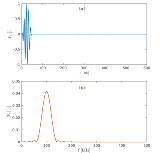
\includegraphics[width=0.95\textwidth]{Chapter_5/excitation}
	\end{center}
	\caption{The 5-cycle signal excitation at carrier frequency \(fc=100\) \unit{\kHz} (\textbf{a}) in the time domain, (\textbf{b}) in the frequency domain}
	\label{fig:signal_100kHz}
\end{figure}
 \section{Sample configuration}
\label{sec:sample}

The sample of interest was a \numproduct{500 x 500 x 1.5} \unit{\cubic\mm} unidirectional \ac{cfrp} plate with stack sequence \(\left[\ang{0},\,\ang{90}\right]_s\) bonded to an aluminium honeycomb core.
The volume fraction of fibres was assumed 47\%.
It was decided to use only one skin, as it is pictured in Figure~\ref{fig:honeycomb}(\textbf{b}), with the intention of experimental validation and to be able to enlarge disbonds between the skin and the core located in the middle of \ac{hsc} with a tool in a real sample. 
However, separate samples were not dedicated for each size of damage because too many factors would affect the signal value, including skin and sensors properties, the thickness of the adhesive layers, position of the core relative to the sensors, and distance between sensor.
Moreover, it renders closely the realistic scenario of monitoring the same structure.
\begin{figure}[H]
	\begin{center}
		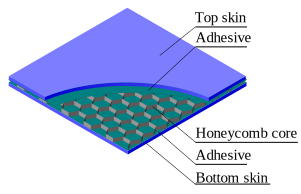
\includegraphics[width=0.95\textwidth]{Chapter_5/honeycomb}
	\end{center}
	\caption{Sample configuration: (\textbf{a}) top view of the sample, (\textbf{b}) \acl{hsc} and (\textbf{c}) details of the honeycomb cell}
	\label{fig:honeycomb}
\end{figure}

The core geometry is accurately reproduced from the actual specimen, i.e., geometry of irregular hexagonal cells \(\left(\mathrm{h}_1 \ne \mathrm{l}_1\right)\) and double walls at the sheet joints, resulting from the core fabrication technology.
According to the drawing in Figure \ref{fig:honeycomb}(\textbf{c}), the cell dimensions are \(\mathrm{w}_c\)=0.1 \unit{\mm}, h\(_1\)=11 \unit{\mm}, h\(_2\)=5 \unit{\mm}, l\(_1\)=10.4 \unit{\mm}, l\(_2\)=6 \unit{\mm} and the cell height g=14.5 \unit{\mm}.
The core was bonded to one \ac{cfrp} plate using the epoxy adhesive (Loctite EA3479B) with the thickness h\(_a\)=0.3 \unit{\mm}.
The adhesive layer covered the entire bottom surface of the skin.
\nomtypeR[w_core]{\(\mathrm{w}_c\)}{Core wall thickness}{}{\unit{\metre}}\nomtypeR[h_core]{h\(_1\), h\(_2\)}{Core cell lengths}{}{\unit{\metre}}\nomtypeR[l_core]{l\(_1\), l\(_2\)}{Core cell widths}{}{\unit{\metre}}\nomtypeR[g_core]{g}{Cell height}{}{\unit{\metre}}\nomtypeR[h_adh]{h\(_a\)}{Adhesive layer thickness}{}{\unit{\metre}}\nomtypeR[h_pzt]{h\(_{PZT}\)}{Transducer thickness}{}{\unit{\metre}}\nomtypeG[phi_pzt]{\(\Phi_{PZT}\)}{Transducer diameter}{}{\unit{\metre}}\nomtypeR[h_glue]{h\(_g\)}{Cyanoacrylate glue thickness}{}{\unit{\metre}}Signal excitation and recording were accomplished with a pair of \acp{pzt}  (Noliac, NCE51) mounted to the top surface of the skin with cyanoacrylate glue.
The circular transducers of diameter \(\Phi_{PZT}\)=10 \unit{\mm} and thickness h\(_{PZT}\)=0.5 \unit{\mm} were attached 200 \unit{\mm} apart, as shown in Figure~\ref{fig:honeycomb}(\textbf{a}).
The thickness of cyanoacrylate glue under the \ac{pzt} was assumed to be h\(_g=50\) \unit{\micro\m}.

The material properties of the components assumed for the simulations are compiled in Table~\ref{tab:properties}.
The effective properties of the \ac{cfrp} skin were determined according to the rule of mixtures presented in the book by Vinson and Sierakowski \cite{vinson1993behavior}.
The authors provide a complete description of the homogenisation of composite properties.
Firstly, the stiffness matrix is determined for the single ply of the laminate along the fibre direction.
Then, the stiffness matrix is transformed for other orientations of the laminate plies by the transformation matrix composed of the direction cosines.
In the analysed sample, there are plies with an orientation of \ang{0} and \ang{90}.
Finally, all the plies in the laminate are homogenised through the thickness.
Sun and Li \cite{sun1988three} present the explicit expressions of the stiffness components for the laminate modelled by solid elements.
The comprehensive equations to derive the effective stiffness matrix are given in Appendix~\ref{app:eff_properties}, whereas Table~\ref{tab:properties_eff} shows the resulting \ac{cfrp} properties.
\begin{table}[H]
	\centering
	\small
	\tabcolsep=0.25cm
	\caption{\label{tab:properties_eff} The homogenised mechanical properties of the \acs{cfrp} plate and the honeycomb core for +20\unit{\degreeCelsius}}
	\begin{tabular}{ccccccccc}
		\toprule
		\multirow{2}{*}{\textbf{Material}} & \(\boldsymbol{E_{11}}\) & \(\boldsymbol{E_{22}}\) & \(\boldsymbol{E_{33}}\) & \(\boldsymbol{G_{12}}\) & \(\boldsymbol{G_{23}}\) & \(\boldsymbol{\nu_{12}}\)	& \(\boldsymbol{\nu_{23}}\) & \(\boldsymbol{\rho}\) \\
		& \unit{\giga\pascal} & \unit{\giga\pascal} & \unit{\giga\pascal} & \unit{\giga\pascal} & \unit{\giga\pascal} & -- & -- & \unit[per-mode = symbol]
		{\kilogram\per\cubic\metre}\\
		\midrule
		\ac{cfrp} & 69.5 & 69.5 & 8.16 & 3.43 & 2.96 & 0.03 & 0.37 & 1555\\
		laminate & & & & & & & &\\
		\midrule
		honeycomb & 0.007 & 0.005 & 2.76 & 0.002 & 0.86 & 0.999 & \(\approx0\) & 112\\
		core & & & & & & & &\\
		\bottomrule
	\end{tabular}
\end{table}
\nomtypeR[G]{\(G\)}{Shear modulus}{}{\unit{\giga\pascal}}% \section{Mesh generation for the \acl{fcgm}}
\label{sec:honeycomb}

The modelled structure was composed of the following components: 2D for the core, epoxy adhesive and cyanoacrylate glue and 3D for the \ac{cfrp} plate and the \acp{pzt}.
Figure~\ref{fig:struct_mesh} depicts the spectral element used to model the wall, the skin and the \ac{pzt}.
During the creation of the core mesh, special attention was taken to minimise the number of non-zero values in the matrix \(\textbf{G}\).
\begin{figure}[H]
	\begin{center}
		\includegraphics[width=0.95\textwidth]{Chapter_5/struct_mesh}
	\end{center}
	\caption{The mesh with the nodes distribution, (\textbf{a}) spectral element used for modeling the wall of the core, (\textbf{b}) excerpt of the skin plate and (\textbf{c}) cyanoacrylate glue mesh with the second-order curve at the boundary}
	\label{fig:struct_mesh}
\end{figure}

The core elements were selected for the slave mesh, with one spectral element dedicated to each honeycomb cell wall.
The master meshes of the skin panel and adhesive layer were divided by three rhombic elements into the area under the core cell.
This way, the interface nodes coincide with those on the hexagon edges (red line in Figure~\ref{fig:struct_mesh}(\textbf{b})).
The map of element nodes and their coordinates were generated by custom code developed in Matlab.
The resulting meshes of the core, adhesive layer and skin are shown in Figure \ref{fig:cas_mesh}.

The mesh for the cyanoacrylate adhesive consisted of five elements, with a second-order curve at the structure boundary, as seen in Figure~\ref{fig:struct_mesh}(\textbf{c}).
This structure was connected to the skin with the non-matching interface elements with the adhesive mesh selected as a slave one.
The \ac{pzt} mesh coincides with the glue mesh and they are connected with the matching interface elements.

\begin{figure}[H]
	\begin{center}
		\includegraphics[width=0.95\textwidth]{Chapter_5/cfrp_mesh}
	\end{center}
	\caption{The meshes of \acl{hsc} components}
	\label{fig:cas_mesh}
\end{figure}
 \section{\Acl{hcgm}}
\label{sec:homogenised}

Section \ref{sec:modelling} contains several examples of the successful application of the model to numerical analysis of \ac{gw} propagation and damage localisation in \ac{hsc}.
Its unquestionable advantage is the simplified component mesh, reducing operating memory resources.
In the dissertation, comparative studies between the \ac{hcgm} and the \ac{fcgm} were conducted to assess the simplified model effectiveness in estimating damage size.

In the \ac{hcgm}, the values of the material constants of the panel core were calculated according to the method presented by Malek and Gibson \cite{malek2015effective}.
This model is an extension of the theoretical analysis of Gibson et al. \cite{gibson1982mechanics}, considering the different geometry of the cell and the nodes at the intersection of the vertical and inclined walls.

The comprehensive formulation of the stiffness matrix components is given in Appendix~\ref{app:eff_properties} and the effective mechanical properties are gathered in Table \ref{tab:properties_eff}.
The properties for other structures, i.e., the skin, the epoxy adhesive, the cyanoacrylate glue, and the sensors remained unchanged.
The core element has \(6 \times 6 \times 4\) nodes, and the mesh coincides with the skin mesh.
The elements of the other structures are the same as described in the previous Section. \section{Damaged structure implementation}
\label{sec:disbond}
The skin and the core disbonds were evaluated to analyse the effect of damage on GW propagation.
A rectangular region of disbonds was investigated with the length along the wave propagation varying in width \(\mathrm{w_d} = [0,10,30,50,70,100,120]\) mm, and the damage length in the perpendicular direction was constant \(\mathrm{l_d} = 170\) mm.
The rectangle was centrally located between the transducers, as presented in Figure~\ref{fig:honeycomb}(\textbf{a}).
The selected dimensions of the defects correspond to the dimensions of disbonds made in the specimen to be measured experimentally.
The damage was done with a sharp hooked tool that detached the core from the adhesive layer cell by cell.
The dimensions of the disbond had a coarse tolerance, measuring the width by a calliper.
Due to the small aluminium sheet thickness, the core cells were squashed within the damaged area.

There were two kinds of disbond models under consideration.
The core cells were removed from the damaged area in the first model as in the mesh pictured in Figure~\ref{fig:disbond}(\textbf{b}).
Whereas in the second model, all components were intact, and only the interface elements between the adhesive layer and the core were decoupled within the yellow area indicated in Figure~\ref{fig:disbond}(\textbf{c}).
\begin{figure}
	\begin{center}
		\includegraphics[width=0.9\textwidth]{Chapter_5/disbond}
	\end{center}
	\caption{The damaged area in the: (\textbf{a}) experimental sample,(\textbf{b}) numerical model with removed cells and (\textbf{c}) numerical model with interface decoupling}
	\label{fig:disbond}
\end{figure} \section{Convergence tests of the solution}
\label{sec:convergence}



\subsection{Spatial convergence}
Spatial convergence was determined after simulations for samples with elements of different order of the Legendre polynomial (see Eq. (\ref{eq:nodes})).
The polynomial order for the \(\xi\times \eta\) plane in the local reference system was changed in the set: \(p=[4,\,5,\,7,\,9,\, 11]\).
The exact order was assumed for each component to minimise the non-zero value of coupling matrix \(\textbf{G}\).
Due to the perpendicularity of the core elements to the skin, the nodes along the core thickness are fixed to 5.
The percentage error was assumed as a criterion for convergence:
\begin{eqnarray}
	\delta^{\mathrm{conv}} = \frac{\sum{\left(e^{\mathrm{max}}-e^{p}\right)^2}}{\sum{\left(e^{max}\right)^2}} \times 100\%,
	\label{eq:perc_err_conv}
\end{eqnarray}
where \(e^{max}\) and \(e^{p}\) are the signal envelopes for the case with the elements of \(11^{\mathrm{th}}\) polynomial order and the observed case, respectively.
A 5\% threshold was assumed for selecting the degree of the polynomial.
The signal envelope is obtained using the Hilbert transform, presented by \cite{staszewski2004health} as:
\begin{eqnarray}
	\label{eq:hilbert}
	\hat{x}(t) &=& \frac{1}{\pi}\int_{-\infty}^{+\infty}x(\tau)\frac{1}{t-\tau}\diff\tau,\\
	\label{eq:envelope}
	e(t) &=& \sqrt{x^2(t)+\hat{x}^2(t)}.
	\nomtypeD[e]{\(e(t)\)}{Signal envelope}{}\nomtypeR[t]{\(t\)}{Time vector}{}{\unit{\second}}\end{eqnarray}

Figure \ref{fig:dx_conv}(\textbf{a}) shows the example of the simulated signals of 100 \unit{\kHz}.
Despite the good agreement of the wave speed for all cases, the amplitudes converge only for a polynomial of order 7.
Based on the graph in Figure \ref{fig:dx_conv}(\textbf{b}) showing simulation errors, the polynomial of order \(p=7\) was selected for 50 and 100 \unit{\kHz} signals, and order \(p=9\) was selected for the 150 \unit{\kHz} signal.
 
Table \ref{tab:elements_nodes} contains a complete list of elements with the number of nodes on each axis \(\xi\times \eta \times \zeta\) which were assumed in simulations.
\begin{figure}[H]
	\begin{center}
		\includegraphics[width=0.95\textwidth]{Chapter_5/dx_conv}
	\end{center}
	\caption{Spatial convergence for the specimen, (\textbf{a}) the sensor signals of 100 \unit{\kHz} for the elements with various polynomial order, (\textbf{b}) percent error for the differ polynomial order}
	\label{fig:dx_conv}
\end{figure}
\begin{table}[H]
	\small
	\tabcolsep=0.5cm
	\centering
	\caption{\label{tab:elements_nodes}The node numbers of the sample components}
	\begin{tabular}{cccc}
		\toprule
		\multirow{3}{*}{\textbf{Component}} & \multicolumn{3}{c}{\textbf{Number of element nodes}}\\
		& \multicolumn{3}{c}{\(n\times m \times l\)}\\
		& \multicolumn{2}{c}{50 \unit{\kHz} 100 \unit{\kHz}} & 150 \unit{\kHz}\\
		\midrule
		Core & \multicolumn{2}{c}{\numproduct{8 x 5 x 1}} & \numproduct{10 x 5 x 1}\\
		Adhesive layer & \multicolumn{2}{c}{\numproduct{8 x 8 x 1}} & \numproduct{10 x 10 x 1}\\
		Skin & \multicolumn{2}{c}{\numproduct{8 x 8 x 4}} & \numproduct{10 x 10 x 1}\\
		Glue & \multicolumn{2}{c}{\numproduct{8 x 8 x 1}} & \numproduct{10 x 10 x 1}\\
		\ac{pzt} & \multicolumn{2}{c}{\numproduct{8 x 8 x 3}} & \numproduct{10 x 10 x 3}\\
		\bottomrule
	\end{tabular}
\end{table}

While the maximum length of the skin element is 6 \unit{\mm}, such a \ac{cfrp} model satisfies the condition of at least six nodes per wavelength for the \ac{a0}, as it is the shortest mode propagating in the assumed frequency range.
Table~\ref{tab:wavelength} shows the \ac{a0} wavelengths for various frequency and propagation angles.
\begin{table}[H]
	\small
	\tabcolsep=0.5cm
	\centering
	\caption{\label{tab:wavelength}The wavelength of the \ac{a0} mode propagated in the presented \ac{cfrp} plate}
	\begin{tabular}{cccccc}
		\toprule
		\textbf{Propagation angle} & \ang{0} & \ang{30} & \ang{45} & \ang{60} & \ang{90}\\
		\textbf{Frequency} [\unit{\kHz}] & \multicolumn{5}{c}{\textbf{Wavelength} [\unit{\mm}]}\\
		\midrule
		50 & 16.5 & 15.2 & 15.0 & 15.2 & 16.6\\
		100 & 10.3 & 9.6 & 9.5 & 9.6 & 10.3\\
		\bottomrule
		\multicolumn{6}{r}{{\scriptsize{source: Dispersion Calculator v1.9}}}
	\end{tabular}
\end{table}
\subsection{Temporal convergence}
A temporal convergence test was conducted to select the appropriate time step value.
The critical value of time increment (\(\Delta t_{cr}\)) depends on the mesh size and the wave mode velocity.
For the explicit time integration algorithm and in accordance with the Courant-Fredrichs-Levy convergence condition, the time step must be less than the ratio of \(\Delta x/c_p\), where \(\Delta x\) is the shortest distance between nodes and \(c_p\) is the phase velocity of the propagating wave.
While time step is set over (\(\Delta t_{cr}\)), the structure displacements increase to infinity immediately as presented in Figure~\ref{fig:dt_cr}.
It indicates that the time step has to be further decreased which can be easily implemented to verify the stability of the attempt.
\begin{figure}[!tbh]
	\begin{center}
		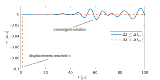
\includegraphics[width=0.95\textwidth]{Chapter_5/dt_cr}
	\end{center}
	\caption{The plate displacement at a point of 50 mm away from actuator in the case of correctly and incorrectly selected time increments}
	\label{fig:dt_cr}
\end{figure} 
\section{Conclusions}
\label{sec:conclusionsSimul}

The Chapter describes the whole model configuration for numerical simulations.
The mesh generation for each component, the excitation signals, and the description of damage modelling are included.
A comparison between the \ac{fcgm} and \ac{hcgm} is also provided.

An essential issue in numerical modelling is the convergence of the solution in the spatial and temporal domains.
Incorrectly selected model parameters cause significant errors in the results.
When a time increment is set over the critical value, displacements tend immediately to infinity.
The size and order of the spectral element should be selected depending on the smallest propagating wavelength in the analysed structure.
In turn, the smallest distance between nodes affects the critical value of the time step.
All this has a consequence on the duration of computer simulations.\clearpage{}
\clearpage{}

\chapter{Experimental Validation of developed models}
\label{ch:validation}

The Chapter includes an assessment of the accuracy and reliability of the modelled physical processes.
In order to validate the sensor model, the frequency characteristic of \ac{emi} was determined through numerical simulations.
The characteristic was then compared with values obtained by theoretical analysis and with experimental measurements.
On the other hand, \ac{hsc} panel model was evaluated experimentally in two ways: by analysing the full wavefield obtained by the \ac{sldv} and by studying the time signals measured by the \acp{pzt} setup.
\section{Validation of the \acl{pzt} model}
\label{sec:pztVal}

The current model, i.e. the curved boundary geometry approximated with the second-order elements, is validated by comparing the transducer impedance obtained by numerical simulation with (i) analytical model and (ii) experimental results.

The impedance Z is a ratio between voltage \((\Phi)\) and current \((I)\) defined as follows
\begin{eqnarray}
	Z = \frac{\Phi}{I} = \frac{\Phi}{i\omega Q},
	\label{eq:impedance}
\end{eqnarray}
\nomtypeG[omega_ang]{\(\omega\)}{Angular frequency}{}{\unit[per-mode = symbol]{\radian\per\second}}\nomtypeR[I]{\(I\)}{Electric current}{}{\unit{\ampere}}\nomtypeD[i]{\(i\)}{Imaginary number}{}\nomtypeR[z_impedance]{\(Z\)}{Impedance}{}{\unit{\ohm}}where \(i=\sqrt{-1}\), \(\omega\) is the angular frequency.
In the case of numerical simulation, \(\Phi\) is assumed as the 1.5-cycle Hann windowed sine pulse at carrier frequency 150 \unit{\kHz}, and \(Q\) is the charge induced on the electrode calculated by Eq. (\ref{eq:pzt_sem}).
The excitation signal has significant values in the 0-300 \unit{\kHz} frequency range, as shown in Figure~\ref{fig:impedance}(\textbf{a}).
The simulations has been conducted according to the \ac{sem} model of the \ac{emi}, implemented in \cite{fiborek2018time}.

The analytical model derived by Giurgiutiu \cite{giurgiutiu2009micromechatronics} is defined as
\begin{eqnarray}
	Z = \frac{1}{i\omega C_0}\left[\left(1-k_p^2\right)+k_p^2\frac{u_r}{u_I}\right],
\end{eqnarray}
\nomtypeR[Capaci]{\(C_0\)}{Transducer free capacitance}{}{\unit{\farad}}\nomtypeD[kp]{\(k_p\)}{Transducer planar coupling coefficient}{}where \(C_0\) is the free capacitance of the sensor, \(k_p\) is the planar coupling coefficient, \(u_r\) is the displacement response, and \(u_I\) is the induced displacement.
Additionally, for comparison, the response of the \ac{sem} with curved boundary approximated by linear elements was included.
All models refer to the free transducer shown in Figure \ref{fig:hioki}(\textbf{a}), i.e. soldered wires and thin electrode coatings have been omitted.

\begin{figure}[H]
	\begin{center}
		\includegraphics[width=0.95\textwidth]{Chapter_6/hioki}
	\end{center}
	\caption{Setup for impedance measurement, (\textbf{a}) Hioki impedance analyser, (\textbf{b}) free \acl{pzt}, (\textbf{c}) with soldered wires ready for measurements}
	\label{fig:hioki}
\end{figure}
For experimental validation, an impedance analyzer (Hioki, IM 3570) was used to determine the electric current flowing through the transducer under the influence of applied voltage in the form of a sine signal with a variable frequency in the range of 1-300 \unit{\kHz}.
Both characteristics are used to determine the impedance according to Eq. (\ref{eq:impedance}).
The measurements were taken at room temperature and averaged 50 times to improve the signal-to-noise ratio.

\begin{figure}[H]
	\begin{center}
		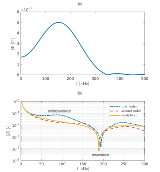
\includegraphics[width=0.95\textwidth]{Chapter_6/impedance}
	\end{center}
	\caption{Validation of the \acl{pzt} model (\textbf{a}) the frequency spectrum of the excitation signal, (\textbf{b}) impedance response of the transducer for numerical model with first order approximation of the boundary (dash-dot red line), numerical model with second order approximation of the curved boundary (dashed blue line), analytical model (dotted yellow line) and experimental measurements (solid purple line)}
	\label{fig:impedance}
\end{figure}

It can be noticed in Figure~\ref{fig:impedance}(\textbf{b}) that the impedance of the model with second order approximation elements is in very good agreement with the analytical solution and to experimental results to the resonance peak.
The resonant peak occurred near 190 \unit{\kHz} for second order model and analytical one and 194 \unit{\kHz} in case of experimental measurement.
The model with a first-order approximation is a better fit for the experiment in frequencies above the resonant peak.
In addition, as opposed to the previous two models and analytical result, an additional antiresonance peak occurred around 90 \unit{\kHz}.

The discrepancy in impedance based on the models and experiment may be due to uncontrolled ambient condition during the measurements and accuracy of piezo- and electromechanical properties provided by the manufacturer. 
Additionally, the models were simplified by excluding the wires and solder unlike the tested transducer shown in Figure \ref{fig:hioki}(\textbf{b}). \section{Experimental setup for \acl{hsc} model validation}
\label{sec:setup}
\begin{figure}[!htb]
	\begin{center}
		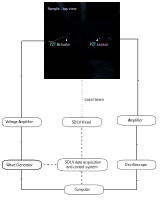
\includegraphics[width=0.95\textwidth]{Chapter_6/setup}
	\end{center}
	\caption{Experimental setup for (1) the \acf{sldv} measurement (dashed line), and (2) the \acf{pzt} wave acquisition (solid line)}
	\label{fig:setup}
\end{figure}
Results from two experimental studies validated the presented model of \ac{hsc}.
The first study was performed for determination of the full wavefield of the propagating waves by the \ac{sldv} (Polytec PSV–400).
The second one was performed for wave acquisition by the \ac{pzt} sensor.
A schematic of the experimental setup is shown in Figure~\ref{fig:setup}.

The \ac{sldv} is method for non-contact measurement of the vibration velocity of structure surface \cite{staszewski2004structural}.
The principle of vibrometer operation is based on the Doppler effect, recording the change of frequency of the light beam reflected from the vibrating surface.
In laser vibrometry, the measurement of frequency change is realised by interferometer and analysis of both reference and measurement light beam.
The measuring system is additionally equipped with mirrors allowing to change the angle of the measuring beam, so it is possible to take measurements at a grid of points on a surface of inspected structural element automatically.
The \ac{sldv} setup is presented in Figure~\ref{fig:sldv}.
\begin{figure}[!htb]
	\begin{center}
		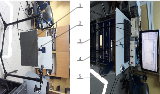
\includegraphics[width=0.95\textwidth]{Chapter_6/sldv}
	\end{center}
	\caption{The \acl{sldv} setup: 1 - the laser sensor head, 2 - the \acl{hsc} specimen, 3 - the arbitrary waveform generator, 4 - the amplifier, 5 - data management system}
	\label{fig:sldv}
\end{figure}

The \ac{pzt} elastic wave generation and acquisition system is used to measure the voltage changes of transducers due to their mechanical deformation.
It is a point measurement at the point of sensor placement.
A data management unit is responsible for executing prepared tasks and collecting data recorded during measurements.
An arbitrary waveform generator is the source of the low voltage signal, which feeds the Lamb wave detection system and high voltage amplifier.
The amplified signal is intended for the actuator to excite a wave in the sample.
The registered signals by the sensor are amplified by the charge amplifier and supplied to an oscilloscope via a splitter.
The setup used for measurements is shown in Figure~\ref{fig:pzt_setup}.
\begin{figure}[!htb]
	\begin{center}
		\includegraphics[width=0.95\textwidth]{Chapter_6/pzt_setup}
	\end{center}
	\caption{The \acl{pzt} setup, (\textbf{a}) the elastic wave generation and acquisition instruments:  DMU - the data management unit, G1,G2 - the arbitrary wave generator, O - the oscilloscope, HVA - the high voltage amplifier, LWDS - the Lamb Wave Detection Systems, (\textbf{b}) the specimen with the \acfp{pzt}}
	\label{fig:pzt_setup}
\end{figure}

Both methods have some advantages and disadvantages, listed in Table~\ref{tab:method_comp}.
The greatest advantage of the \ac{sldv} technique is the non-contact surface measurements.
If three heads of the laser sensor are available then three-axes of velocity measurements are possible.
However, this method is unsuitable for in-service testing of structures due to its large size and the need to guarantee conditions that prevent signal interference. Therefore, \ac{sldv} is often used in laboratory conditions or when the facility is in maintenance mode.
On the other hand the \ac{pzt} setup is a rather low cost instruments for spot recording of the wave propagation.
The measurements are characterized by high repeatability and can be performed on the construction in operation.

\begin{table}[!htb]
	\small
	\tabcolsep=0.2cm
\caption{\label{tab:method_comp}Comparison of methods for elastic wave propagation measurements}
	\begin{tabular}{p{0.1\textwidth}>{\raggedright}p{0.4\textwidth}>{\raggedright \arraybackslash}p{0.4\textwidth}}
		\toprule
		\textbf{Method} &\textbf{Advantages} & \textbf{Disadvantages}\\
		\midrule
		\multirow{5}{*}{\ac{sldv}}   & \tabitem automatic full-field scanning & \tabitem high-cost equipment\\ 
		& \tabitem non-contact measurement & \tabitem low signal-to-noise ratio\\
		& \tabitem \ac{3d} velocity vector (optional)& \tabitem special surface treatment is needed, e.g. application of retro-reflective tape\\
		& & \tabitem relatively large space need for measurements \\
		& & \tabitem special sample mounting for repeatability of measurements\\
		\midrule
		\multirow{5}{*}{\ac{pzt}} & \tabitem low-cost instruments & \tabitem spot measurement\\
		& \tabitem high repeatability of measurements & \tabitem displacements vector correlated with the sensor polarization\\
		& \tabitem measurements on the sample in motion & \tabitem cumbersome wiring\\
		& \tabitem generation and recording signals with the same setup & \tabitem sensitive to electric and magnetic fields\\		
		\bottomrule
	\end{tabular}
\end{table}

The specimen comprised of components described in Section~\ref{sec:sample} was fabricated under workshop conditions with rough accuracy.
Before applying the two-ingredient glue (Loctite EA3479B), the bottom surface of the skin was cleaned and degreased with the solvent (Loctite SF7063).
The adhesive curing took 48 hours under a distributed load at ambient temperature.
The top view of the sample is presented in Figure~\ref{fig:sample_dim}.
\begin{figure}[!htb]
	\begin{center}
		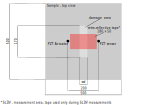
\includegraphics[width=0.95\textwidth]{Chapter_6/sample_dim}
	\end{center}
	\caption{Schematic image of the sample}
	\label{fig:sample_dim}
\end{figure}

The subject of the parametric study was the effect of the disbond size on the propagating \ac{gw}.
A reference measurement of an intact sample was followed by several measurements taken for the subsequent damage introduced on the same specimen.
The damage width varied in range \(\mathrm{w_d}=\left [10, 30, 50, 70, 100, 120 \right ]\) \unit{\mm}, while its fixed length was \(\mathrm{l_d} = 175\) \unit{\mm}.
\nomtypeR[w_dam]{\(w_d\)}{Damage width}{}{\unit{\metre}}\nomtypeR[l_dam]{\(l_d\)}{Length width}{}{\unit{\metre}}The \(N_c=5\) cycle Hann windowed signal at carrier frequencies \(f_c=[50,100,150]\) \unit{\kHz} was used in the measurements.

The data management unit is used to set measurement parameters, managing them, and saving the collected results.
The arbitrary waveform generator (National Instruments, PXI 1095) generates the low-voltage signal from where it feeds Lamb waves detection system (LWDS, Cedrat Technologies) and the actuator (Noliac, NCE51) after 100 times amplification by the  amplifier (Krohn-Hite Corporation, model 7500).
Voltage of the the sensor (Noliac, NCE51) is measured by the oscilloscope (National Instruments, PXI 1095) through the LWDS.
Each measurement was conducted at the temperature of 20\unit{\degreeCelsius} controlled in the environmental chamber (Angelantoni Test Technologies, DM 600C) and averaged 20~times to improve the signal-to-noise ratio. \section{Results of \acl{hsc} validation with the \acl{sldv} setup}
\label{sec:resuls_sldv}
Figures~\ref{fig:fullfield_50_0}, \ref{fig:fullfield_100_0} and \ref{fig:fullfield_150_0} present the full wavefield in the healthy sample.
The experimental measurements and the \ac{fcgm} snapshots show that the wavefront distortion is rising with the frequency.
Because the wavelength decreases as the frequency increases, a higher frequency signal is more likely to induce wave reflections from the core walls.
This effect can not be observed in the case of the \ac{hcgm}.

\begin{figure}[!hbt]
	\begin{center}
		\includegraphics[width=0.95\textwidth]{Chapter_6/fullfield_50_0}
	\end{center}
	\caption{The top surface out-of-plane velocity snapshots for (\textbf{a}) the \acf{fcgm}, (\textbf{b}) the experimental results obtained by \acf{sldv}, and (\textbf{c}) the \acf{hcgm} in the \textbf{healthy~sample at 50 kHz}}
	\label{fig:fullfield_50_0}
\end{figure}
\begin{figure}[!hbt]
	\begin{center}
		\includegraphics[width=0.95\textwidth]{Chapter_6/fullfield_100_0}
	\end{center}
	\caption{The top surface out-of-plane velocity snapshots for (\textbf{a}) the \acf{fcgm}, (\textbf{b}) the experimental results obtained by the \acf{sldv}, and (\textbf{c}) the \acf{hcgm} in the \textbf{healthy~sample at 100 kHz}}
	\label{fig:fullfield_100_0}
\end{figure}
\begin{figure}[!hbt]
	\begin{center}
		\includegraphics[width=0.95\textwidth]{Chapter_6/fullfield_150_0}
	\end{center}
	\caption{The top surface out-of-plane velocity snapshots for (\textbf{a}) the \acf{fcgm}, (\textbf{b}) the experimental results obtained by the \acf{sldv}, and (\textbf{c}) the \acf{hcgm} in the \textbf{healthy~sample at 150 kHz}}
	\label{fig:fullfield_150_0}
\end{figure}

In case of the damaged sample, the wavefront is not distorted in the damage area bounded by dashed white rectangle in Figures~\ref{fig:fullfield_50_5}, \ref{fig:fullfield_100_5} and \ref{fig:fullfield_150_5} for all three cases.
Due to the lack of wave leakage into the core, the wave propagates smoothly through the skin.
For the experimental sample and the \ac{fcgm}, interference of waves reflected from the cells and the damage boundary is observed.
The wave interference observed in the \ac{hcgm} refers to waves reflected only from the defect.

\begin{figure}[!hbt]
	\begin{center}
		\includegraphics[width=0.95\textwidth]{Chapter_6/fullfield_50_5}
	\end{center}
	\caption{The top surface out-of-plane particle velocity snapshots for (\textbf{a}) the \acf{fcgm}, (\textbf{b}) the experimental results obtained by the \acf{sldv}, and (\textbf{c}) the \acf{hcgm} \textbf{with removed core elements at 50 kHz} in damaged area for both numerical models}
	\label{fig:fullfield_50_5}
\end{figure}
\begin{figure}[!hbt]
	\begin{center}
		\includegraphics[width=0.95\textwidth]{Chapter_6/fullfield_100_5}
	\end{center}
	\caption{The top surface out-of-plane velocity snapshots for (\textbf{a}) the \acf{fcgm}, (\textbf{b}) the experimental results obtained by the \acf{sldv}, and (\textbf{c}) the \acf{hcgm} \textbf{with removed core elements at 100 kHz} in damaged area for both numerical models}
	\label{fig:fullfield_100_5}
\end{figure}
\begin{figure}[!hbt]
	\begin{center}
		\includegraphics[width=0.95\textwidth]{Chapter_6/fullfield_150_5}
	\end{center}
	\caption{The top surface out-of-plane velocity snapshots for (\textbf{a}) the \acf{fcgm}, (\textbf{b}) the experimental results obtained by the \acf{sldv}, and (\textbf{c}) the \acf{hcgm} \textbf{with removed core elements at 150 kHz} in damaged area for both numerical models}
	\label{fig:fullfield_150_5}
\end{figure}
\clearpage \section{Results of \acl{hsc} validation with \aclp{pzt} wave acquisition setup}
\label{sec:resuls_pzt}
Validation of the honeycomb structure models and a separate \ac{cfrp} plate intended for \ac{hsc} sample were done by comparing the group velocity and amplitude of the first packet of \ac{s0} and \ac{a0} arriving at the sensor.
Figure~\ref{fig:signal_exp_raw} contains examples of the experimentally obtained raw signals for the healthy and damaged samples.
The raw signals are processed for noise reduction and next an envelope of the signals is calculated.
The envelope is used to obtain the amplitude and group velocity of the mods for the model validation and is used in the analytical assessment of damage magnitude.
\begin{figure}[!htb]
	\begin{center}
		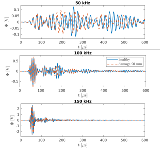
\includegraphics[width=0.95\textwidth]{Chapter_6/signal_exp_raw}
	\end{center}
	\caption{Raw signals registered by the sensor in \acl{hsc} for the specimen at healthy state and the state with 90 \unit{\mm} width damage}
	\label{fig:signal_exp_raw}
\end{figure}

Signal processing follows the diagram shown in Figure~\ref{fig:signal_processing}.
A preliminary step is a conversion of the signals from the time domain to the frequency domain by the \ac{fft}.
Then, the band-pass filter is applied in the range \(0.5f_c-1.5f_c\).
For this purpose a Butterworth filter of 20th order was used.
After filtering, the signal is converted back to the time domain by the \ac{ifft}.
Lastly, the envelope of the signal \(e(t)\) is obtained using Eq. (\ref{eq:envelope}).

\begin{figure}[!htb]
	\begin{center}
		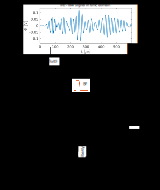
\includegraphics[width=0.95\textwidth]{Chapter_6/signal_processing}
	\end{center}
	\caption{Raw signals registered by the sensor in \acl{hsc} for healthy state and damage of 90 \unit{\mm} width}
	\label{fig:signal_processing}
\end{figure}

The group velocity is derived from the signal envelope related to particular Lamb wave mode and its \ac{tof}.
The \ac{tof} is a difference between the arrival of the maximum amplitude of the envelope of considered mode at the sensor \((\mathrm{T}_1)\) and the half time of the excitation pulse \(\left(\mathrm{T}_0=\frac{1}{2f_m}\right)\).
Since the distance between the transducers is constant \(l=200\) \unit{\mm}, the group velocity equals
\begin{eqnarray}
	C_g = \frac{\mathrm{ToF}}{l}=\frac{T_1-T_0}{l}.
\end{eqnarray}

The signal envelopes are shown in Figure~\ref{fig:single_skin} for single \ac{cfrp} plate, Figure~\ref{fig:hsc_full} for the \ac{fcgm}, and Figure~\ref{fig:hsc_homo}, from which the velocities and amplitudes of the wave mods were determined.
\begin{figure}[!htb]
	\begin{center}
		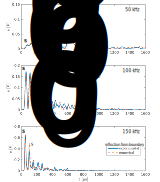
\includegraphics[width=0.95\textwidth]{Chapter_6/single_skin}
	\end{center}
	\caption{The signal envelope for single \acs{cfrp} skin; experimental vs. numerical simulation}
	\label{fig:single_skin}
\end{figure}
\begin{figure}[!htb]
	\begin{center}
		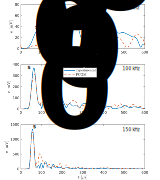
\includegraphics[width=0.95\textwidth]{Chapter_6/HSC_full}
	\end{center}
	\caption{The signal envelope for the \acl{hsc} structure; experimental vs. the \acf{fcgm}}
	\label{fig:hsc_full}
\end{figure}
\begin{figure}[!htb]
	\begin{center}
		\includegraphics[width=0.95\textwidth]{Chapter_6/HSC_homo}
	\end{center}
	\caption{The signal envelope for the \acl{hsc} structure; experimental vs. the \acf{hcgm}}
	\label{fig:hsc_homo}
\end{figure}

For the single \ac{cfrp} plate, Table~\ref{tab:group_velocity_cfrp} gives the determined velocities and amplitudes of the modes together with the percentage errors defined by
\begin{eqnarray}
	\delta = \left|\frac{x^{num}-x^{exp}}{x^{exp}}\right|\times100\%,
	\label{eq:perc_err}
\end{eqnarray}
\nomtypeG[delta]{\(\delta\)}{Percentage error}{}{\%}where \(x^{num}\) and \(x^{exp}\) are the numerical and experimental values, respectively.
It can be noticed that the model is in good agreement with experimental results.
All values are within an error of up to 10\%, except for the \ac{s0} and \ac{a0} amplitudes for 50 and 100 \unit{\kHz}, respectively.
For these cases, the error is about 25\%.
The \ac{a0} mode at 150 \unit{\kHz} in Figure~\ref{fig:hsc_homo} was not identified because the high amplitude \ac{s0} reflections mask it.

Regarding \ac{hsc} panel, the best results are achieved for the \ac{fcgm} as it is shown in Table~\ref{tab:group_velocity_hsc}.
The velocity error is less than 10\% for both modes except for the signal at 50 \unit{\kHz}. 
In the case of signals amplitude, the simulation results are underestimated.
Only the \ac{s0} at 100 and 150 \unit{\kHz} has the error less than 15\%.
For the \ac{hcgm}, the best result are obtained for the \ac{s0} at 150 \unit{\kHz} with error less than 11\%.
Amplitudes of the \ac{a0} for this model are more accurate than the \ac{fcgm} with the errors below 15\%.

\begin{table}[!htb]
	\small
	\tabcolsep=0.2cm
	\centering
	\caption{\label{tab:group_velocity_cfrp} Comparison between amplitudes and group velocities obtained from the simulations and experiments for the single \acs{cfrp} plate}
	\begin{tabular}{cccccccc}
		\toprule
		& & \multicolumn{3}{c}{\(C_g\)} & \multicolumn{3}{c}{Amp.}\\
		\multirow{2}{*}{Mode} & Frequency & Exp. & Num. & \(\delta\)& Exp. & Num. & \(\delta\)\\
		& \unit{\kHz} & \unit[per-mode = symbol]{\m\per\s} & \unit[per-mode = symbol]{\m\per\s} & \% & \unit{\mV} & \unit{\mV} & \% \\
		\midrule
		\multirow{3}{*}{\ac{s0}} & 50 & 6079 & 5865 & \textcolor{green}{3.52}& 12 & 171 & \textcolor{red}{25.0} \\
		&100& 5571 & 5747 & \textcolor{green}{3.16} & 171 & 162 & \textcolor{green}{5.26}\\
		&150& 5764 & 5698 & \textcolor{green}{1.15} & 648 & 664 & \textcolor{green}{2.47}\\
		\midrule
		\multirow{3}{*}{\ac{a0}} &50& 1341 & 1325 & \textcolor{green}{0.74} & 134 & 125 & \textcolor{green}{6.72}\\
		&100& 1550 & 1396 & \textcolor{green}{9.74} & 84 & 104 & \textcolor{red}{23.8}\\
		&150& \multicolumn{6}{c}{-} \\
		\bottomrule
	\end{tabular}
\end{table}
\begin{table}[!htb]
	\small
	\tabcolsep=0.15cm
	\centering
	\caption{\label{tab:group_velocity_hsc} Comparison between amplitudes and group velocities obtained from the simulations based on the \acf{fcgm} and the \acf{hcgm} and experiments for \acl{hsc}}
	\begin{tabular}{cccccccccccc}
		\toprule
		& & \multicolumn{5}{c}{\(C_g\)} & \multicolumn{5}{c}{Amp.}\\
		\multirow{2}{*}{Mode} & Freq.& Exp. & \ac{fcgm} & \(\delta\) & \ac{hcgm} & \(\delta\) &  Exp. & \ac{fcgm} & \(\delta\) & \ac{hcgm} & \(\delta\)\\
		& \unit{\kHz} & \unit[per-mode = symbol]{\m\per\s} & \unit[per-mode = symbol]{\m\per\s} & \% & \unit[per-mode = symbol]{\m\per\s} & \% & \unit{\mV} & \unit{\mV} & \%& \unit{\mV} & \% \\
		\midrule
		\multirow{3}{*}{\ac{s0}} & 50 & 6452 & 8696 & {34.78} & 8333 & {29.15} & 32 & 6 & \textcolor{red}{81.25} & 3 & \textcolor{red}{90.63}\\
		&100& 5263 & 5128 & \textcolor{green}{2.57} & 5714 & \textcolor{green}{8.57} & 369 & 314 & \textcolor{green}{14.91} & 138 & \textcolor{red}{62.6}\\
		&150& 5085 & 5217 & \textcolor{green}{2.60} & 4959 & \textcolor{green}{2.48} & 1341 & 1239 & \textcolor{green}{7.61} & 1482 & \textcolor{green}{10.51}\\
		\midrule
		\multirow{3}{*}{\ac{a0}} & 50 & 966 & 926 & \textcolor{green}{4.14} & 1316 & {36.23} & 62 & 76 & {22.58} & 63 & \textcolor{green}{1.61}\\
		& 100 & 2174 & 2151 & \textcolor{green}{1.06} & 2273 & \textcolor{green}{4.55} & 137 & 179 & {30.66} & 117 & \textcolor{green}{14.60}\\
		& 150 & \multicolumn{10}{c}{-}\\
		\bottomrule
	\end{tabular}
\end{table}
Errors in the models may be due to several factors.
The most important ones include differences in material properties of used components.
In the models, an average thickness of the adhesive layer was assumed; obtaining precise thickness of the adhesive layer in the specimen preparation is difficult under workshop conditions.
The models also assumed the same shape for each core cell, whereas in practice, the geometry was different because of in-plane deformation of the core during the sample preparation.
The velocity in the panel varies with the angle of propagation due to anisotropy of \ac{cfrp} plate and the geometry of the honeycomb core.
In the models, the direction of wave propagation between the sensors was assumed to coincide with the skin and core orientation.
The speed is also affected by the accuracy of the \ac{pzt} placement. 
\section{Conclusions}
\label{sec:conclusionsValid}

The Chapter presents the validation of the developed models.
The \ac{emi} characteristic of the \ac{pzt} model had a good agreement with analytically obtained characteristic and with experimental results in the analysed frequency range of 0-300 \unit{\kHz}.
The \ac{sldv} analysis showed that \ac{fcgm} expresses better wave propagation behaviour in \ac{hsc} than homogenised model.
The snapshots of the full wavefield showed wave interference in the core cells, which was impossible to obtain in the \ac{hcgm}.
The full-field analysis also showed a lack of wave leakage into the core at the damaged area.
This phenomenon is the basis for determining the effect of the damage on wave propagation.
The velocity of the wave propagation for both models was in good agreement with the \ac{pzt} measurements.\clearpage{}
\clearpage{}\chapter[The Severity of Damage Estimation]{The Severity of Damage Estimation}
\label{ch:severity}

A series of computer simulations were performed for different bond sizes for both the \ac{fcgm} and the \ac{hcgm}.
Two damage models were considered i.e., the removed core cells  and no coupling between the core and the adhesive layer.
The electrical voltage signal captured at the sensor was then analysed to determine the \ac{madif}.
Several \acfp{di} were used to determine the effect of damage on the propagation waveform.
Of all the indices, those that were monotonic in the assumed damage size range and with the most significant change in index value were selected for further consideration.
Then, the results were compared with the corresponding indices obtained experimentally.
Finally, those with the lowest error were selected to determine the \ac{madif}.


\section{Damage indices}
\label{sec:di}

In the dissertation, six damage indices, considered to be the most effective \cite{torkamani2014novel, moix2016damage}, were analysed based on the signal envelope in the time-domain registered by the sensor.
All of them were considered in three variants: (i) the full-length of the signal, (ii) the first wave packet of the \ac{s0}, (iii) the first wave packet of the \ac{a0}.
The analysis considered signals at 50, 100 and 150 \unit{\kHz}, with the last frequency excluded for the \ac{a0}, because, as indicated in Section~\ref{sec:resuls_pzt}, this mode was masked by reflections of the \ac{s0}.
The wave packets were extracted by windowing the full-length signals with a flattened Gaussian window in the form
\begin{eqnarray}
	g(t)= \mathrm{exp}\left(-\left(\frac{t-t_0}{w_g}\right) ^{n}\right),
	\label{eq:psi_g}
\end{eqnarray}
\nomtypeD[gt]{\(g(t)\)}{Gaussian window}{}where \(t_0\) and \(w_g=0.5N_c/f_c\) are the center point and the half-width of the window, respectively, and \(n\) determines the slope of the window. Figure~\ref{fig:windows} depicts the usage of the window.
\begin{figure}[!tbh]
	\begin{center}
		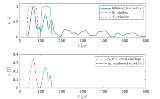
\includegraphics[width=0.95\textwidth]{Chapter_7/windows}
	\end{center}
	\caption{The signal envelop and the Gaussian windows}
	\label{fig:windows}
\end{figure}

The following time-domain indices were taken into consideration: \ac{p2p}, \ac{saps}, \ac{sapr}, \acf{rmsd}, \ac{eng} and \ac{cc}.
Definitions of these metrics are as follows:

\begin{eqnarray}
	\mathrm{P2P} & = & \left(\mathrm{max}(e_H) - \mathrm{max}(e_D)\right),\\
	\mathrm{SAPS} & = & 1 - \left(\frac{\mathrm{max}(e_H)-\mathrm{max}(e_D)}{\mathrm{max}(e_H)}\right)^2,\\
	\mathrm{SAPR} & = & \frac{\mathrm{max}(e_H)}{\mathrm{max}(e_D)},\\
	\mathrm{RMSD} & = & 1 - \sqrt{\frac{\sum_{i=1}^{n}\left[e_D-e_H\right]^2}	{\sum_{i=1}^{n}e_H^2}},\\
	\mathrm{ENG} & = & 1 -  \frac{\sum_{i=1}^{n}{e_D^2}-\sum_{i=1}^{n}{e_H^2}}{\sum_{i=1}^{n}{e_H^2}},\\
	\mathrm{CC} & = & \frac{n\sum_{i=1}^{n}e_De_H-\sum_{i=1}^{n}e_D\sum_{i=1}^{n}e_H}{\sqrt{n\sum_{i=1}^{n}e_D^2-\left[\sum_{i=1}^{n}e_D\right]^2}\sqrt{n\sum_{i=1}^{n}e_H^2-\left[\sum_{i=1}^{n}e_H\right]^2}},
\end{eqnarray}
where \(e_H\) and \(e_D\) are the envelope of the signal registered by the sensor for the healthy and damaged state of the specimen, respectively, and \(n\) is the length of the signal.
The \ac{p2p}, \ac{saps}, \ac{sapr} are based on the difference between amplitudes of the monitored and the baseline state.
The \ac{rmsd} measures the error between baseline and damaged, \ac{eng} compares the difference of the sensor responses energy and \ac{cc} is the index based on Pearson correlation coefficient.

\begin{figure}[!tbh]
	\begin{center}
		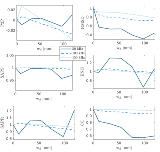
\includegraphics[width=0.95\textwidth]{Chapter_7/DI_full_full}
	\end{center}
	\caption{The \aclp{di} obtained with the \acl{fcgm} based on the full-length signals}
	\label{fig:DI_full_full}
\end{figure}
\begin{figure}[!tbh]
	\begin{center}
		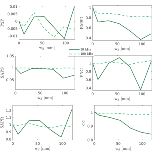
\includegraphics[width=0.95\textwidth]{Chapter_7/DI_full_A0}
	\end{center}
	\caption{The \aclp{di} obtained with the \acl{fcgm} based on the \acs{a0} windowed signal}
	\label{fig:DI_full_A0}
\end{figure}
\begin{figure}[!tbh]
	\begin{center}
		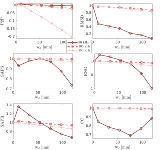
\includegraphics[width=0.95\textwidth]{Chapter_7/DI_full_S0}
	\end{center}
	\caption{The \aclp{di} obtained with the \acl{fcgm} based on the \acs{s0} windowed signal}
	\label{fig:DI_full_S0}
\end{figure}

The \acp{di} based on full-length signals derived from simulations with the \ac{fcgm} are presented in Figure~\ref{fig:DI_full_full}.
The damage was modelled by removing the core cells in the damage area.
Noticeably, all the \acp{di} for 50 \unit{\kHz} are not monotonous.
This is due to the fact that a low-frequency wave (up to 100 \unit{\kHz}, according to work of Tian et al. \cite{tian2015wavenumber}), propagates through the entire thickness of \ac{hsc}.
Therefore, in the analysis of damage size, not only the phenomenon of wave leakage is relevant, but also the reflection from cell walls.  
The high-frequency wave propagates mainly through the skin of the panel, so changes in the signal recorded by the sensor in the damaged sample are mainly caused by the wave leakage effect.

The \acp{di} based on the windowed signals are shown in Figures~\ref{fig:DI_full_A0} and \ref{fig:DI_full_S0} for the \ac{a0} and \ac{s0} window, respectively.
It should be mentioned that \acp{di} for 150 \unit{\kHz} were omitted in Figure~\ref{fig:DI_full_A0}, due to the masking of this mode by the \ac{s0} reflections.
The characteristics of the \ac{s0}-based indices are consistent with the related indices determined for the full-length signals, although for most indices, their values are less than those of full-length signals.
The \ac{s0}-based \acp{di} values are also less than the \ac{a0}-based signals, except the \ac{rmsd} at 50 \unit{kHz}.
It is because dominant displacements of the \ac{s0} are in-plane of the skin, so less portion of the wave energy leak into the core through the healthy region.
In the case of the full-length response, the \ac{a0} was registered, which is more susceptible to damage in the form of disbonds or delamination since its main displacements are out-of-plane.

Accordingly, the following indicators were selected for further consideration: \ac{p2p} and \ac{sapr} at 150 \unit{kHz} (see Figures \ref{fig:DI_P2P} and \ref{fig:DI_SAPR}), \ac{rmsd} and \ac{cc}, all in the case of full-length and at 100 and 150 \unit{\kHz} (see Figures \ref{fig:DI_RMSD_full} and \ref{fig:DI_CC}), and \ac{rmsd} at 50 \unit{kHz} \ac{s0}-based signals (see Figure \ref{fig:DI_RMSD_S0}).
Selected indicators were also determined for damage modeled by removing interface elements. Then, they were compered with the indices obtained for the \ac{hcgm}.

\begin{figure}[!tbh]
	\begin{center}
		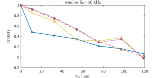
\includegraphics[width=0.95\textwidth]{Chapter_7/DI_P2P}
	\end{center}
	\caption{Comparison of the selected \acfp{p2p} based on full-length signals for the various models of the core and damage: the \acf{fcgm} with removed core cells (solid line), the \acf{fcgm} with removed interface elements (dashed line), the \acf{hcgm} with removed core cells (dash-dot line), the \acf{hcgm} with removed interface elements(dotted line)}
	\label{fig:DI_P2P}
\end{figure}

\begin{figure}[!tbh]
	\begin{center}
		\includegraphics[width=0.95\textwidth]{Chapter_7/DI_SAPR}
	\end{center}
	\caption{Comparison of the selected \acfp{sapr} based on full-length signals for the various models of the core and damage: the \acf{fcgm} with removed core cells (solid line), the \acf{fcgm} with removed interface elements (dashed line), the \acf{hcgm} with removed core cells (dash-dot line), the \acf{hcgm} with removed interface elements (dotted line)}
	\label{fig:DI_SAPR}
\end{figure}
It can be noticed that \ac{p2p} and \ac{sapr} differ significantly in terms of the core model used. Both indexes for the \ac{fcgm} are continuously decreasing, while for the \ac{hcgm}, the values are almost constant in the whole range of damage.
In addition, the damage model has little effect only for the \ac{fcgm}.

\begin{figure}[!tbh]
	\begin{center}
		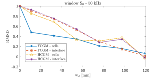
\includegraphics[width=0.95\textwidth]{Chapter_7/DI_RMSD_S0}
	\end{center}
	\caption{Comparison of the selected \acfp{rmsd} based on \ac{s0} windowed signals for the various models of the core and damage: the \acf{fcgm} with removed core cells (solid line), the \acf{fcgm} with removed interface elements (dashed line), the \acf{hcgm} with removed core cells (dash-dot line), the \acf{hcgm} with removed interface elements (dotted line)}
	\label{fig:DI_RMSD_S0}
\end{figure}

The values for all cases are consistent for the \ac{rmsd} based on the \ac{s0} window.
Only the \ac{fcgm} for the two smallest damage scenarios deviates from the other models.
\begin{figure}[!tbh]
	\begin{center}
		\includegraphics[width=0.95\textwidth]{Chapter_7/DI_RMSD_full}
	\end{center}
	\caption{Comparison of the selected \acfp{rmsd} based on full-length signals for the various models of the core and damage: the \acf{fcgm} with removed core cells (solid line), the \acf{fcgm} with removed interface elements (dashed line), the \acf{hcgm} with removed core cells (dash-dot line), the \acf{hcgm} with removed interface elements (dotted line)}
	\label{fig:DI_RMSD_full}
\end{figure}

\begin{figure}[!tbh]
	\begin{center}
		\includegraphics[width=0.95\textwidth]{Chapter_7/DI_CC_full}
	\end{center}
	\caption{Comparison of the selected \acfp{cc} based on full-length signals for the various models of the core and damage: the \acf{fcgm} with removed core cells (solid line), the \acf{fcgm} with removed interface elements (dashed line), line the \acf{hcgm} with removed core cells (dash-dot), the \acf{hcgm} with removed interface elements (dotted line)}
	\label{fig:DI_CC}
\end{figure}

For the \ac{rmsd} and the \ac{cc} based on full-length signals, the results are comparable for the all models, except the values for the \ac{hcgm} at 100 \unit{kHz} are more significant than the \ac{fcgm}.
 \section{Determination of the \acl{madif}}
\label{sec:determination}

The \ac{madif} was determined based on the function best fitted to indices selected in the previous subsection.
Since the numerically obtained indices took the shape of a non-linear function, several curves were assumed to find the best fit.
These functions were defined in the general form as follows
\begin{eqnarray}
	y_1(x,a_i) & = & \frac{a_1x}{x+a_2}+a_3,
	\label{eq:function_1}\\
	y_2(x,a_i) & = & a_1\sqrt{x} + a_2x+a_3,
	\label{eq:function_2}\\
	y_3(x,a_i) & = & \frac{a_1x}{\sqrt{a_2 + a_3x^2}}+a_4,\label{eq:function_3} 
\end{eqnarray}
where \(a_i\) are the coefficients of the functions.
The coefficients were determined by built-in function of Matlab named \verb+fminsearch+, which searches for the minimum of a problem specified by \(\min\limits_a f(x,a)\), and the function to be optimised was assumed to be \(f(x,a)=\left\|DI_{num} - y(x,a_i)\right\|\), where \(\left\|\cdot\right\|\) means Euclidean norm.
A criterion for evaluating the fit of the curve to simulation results was a mean absolute error defined as follows
\begin{eqnarray}
	\delta^{\mathrm{fit}} = \frac{1}{\mathrm{n^{DI}}}\sum_{i=1}^{\mathrm{n^{DI}}} \left|\frac{\mathrm{DI^i_{num}}-y(w_d^i)}{\mathrm{DI^i_{num}}}\right|\times100\%,
\end{eqnarray}
where \(\mathrm{n^{DI}}\) is the number of index points.
The examples of the results for \ac{rmsd} are presented in Table~\ref{tab:fit_RMSD_full_FCGM} based on the \ac{fcgm} and in Table~\ref{tab:fit_RMSD_full_HCGM} for the \ac{hcgm}.
The empty cells in the tables mean that the function was fitted with an error of more than 20\%.
The \ac{di} was no longer taken into account if the fit function was not established.
Although prepared, the presentation of a similar summary for the remaining cases was omitted for the Chapter's clarity.
Ultimately, the most fitted function was Eq.~(\ref{eq:function_1}) and Eq.~(\ref{eq:function_2}) for the most \acp{di}.
The best fitted functions were selected to determine the \ac{madif}.

\begin{table}
	\small
	\tabcolsep=0.1cm
	\centering
	\caption{\label{tab:fit_RMSD_full_FCGM} The errors of the functions fitted to the \acf{rmsd} based on full-length windowed signals and the \acf{fcgm}}
	\begin{tabular}{ccccccccccccccc}
		\toprule
		\multirow{3}{*}{\rotatebox[origin=c]{90}{Frequency}} & \multicolumn{7}{c}{\ac{fcgm} - core} & \multicolumn{7}{c}{\ac{fcgm} - interface}\\
		& \multirow{2}{*}{\rotatebox[origin=c]{90}{DI\(_{num}\)}} & \multicolumn{2}{c}{Eq.~(\ref{eq:function_1})} & \multicolumn{2}{c}{Eq.~(\ref{eq:function_2})} & \multicolumn{2}{c}{Eq.~(\ref{eq:function_3})} &
		\multirow{2}{*}{\rotatebox[origin=c]{90}{DI\(_{num}\)}} & \multicolumn{2}{c}{Eq.~(\ref{eq:function_1})} & \multicolumn{2}{c}{Eq.~(\ref{eq:function_2})} & \multicolumn{2}{c}{Eq.~(\ref{eq:function_3})}\\
		& & \(y(w_d^i)\)& \(\delta^{\mathrm{fit}}\) & \(y(w_d^i)\) & \(\delta^{\mathrm{fit}}\) & \(y(w_d^i)\) & \(\delta^{\mathrm{fit}}\) & & \(y(w_d^i)\)& \(\delta^{\mathrm{fit}}\) & \(y(w_d^i)\) & \(\delta^{\mathrm{fit}}\) & \(y(w_d^i)\) & \(\delta^{\mathrm{fit}}\)\\
		\midrule
		\multirow{7}{*}{\rotatebox[origin=c]{90}{100 \unit{\kHz}}} & 1.00 & 1.00 & \multirow{7}{*}{\rotatebox[origin=c]{90}{\textcolor{green}{1.50}}} & 1.00 & \multirow{7}{*}{\rotatebox[origin=c]{90}{1.70}} & 1.00 & \multirow{7}{*}{\rotatebox[origin=c]{90}{1.92}} & 1.00 & 1.00 & \multirow{7}{*}{\rotatebox[origin=c]{90}{\textcolor{green}{1.11}}} & 1.00 & \multirow{7}{*}{\rotatebox[origin=c]{90}{1.45}} & 1.00 & \multirow{7}{*}{\rotatebox[origin=c]{90}{1.31}} \\
		& 0.83 & 0.85 & & 0.88 & & 0.84 & & 0.92 & 0.92 & & 0.90 & & 0.94 & \\ 
		& 0.82 & 0.80 & & 0.82 & & 0.79 & & 0.85 & 0.84 & & 0.83 & & 0.85 & \\ 
		& 0.80 & 0.78 & & 0.79 & & 0.78 & & 0.79 & 0.79 & & 0.79 & & 0.80 & \\ 
		& 0.76 & 0.78 & & 0.78 & & 0.78 & & 0.76 & 0.77 & & 0.76 & & 0.77 & \\ 
		& 0.77 & 0.77 & & 0.77 & & 0.78 & & 0.73 & 0.75 & & 0.74 & & 0.76 & \\ 
		& 0.75 & 0.77 & & 0.78 & & 0.78 & & 0.75 & 0.73 & & 0.72 & & 0.75 & \\
		\midrule
		\multirow{7}{*}{\rotatebox[origin=c]{90}{150 \unit{\kHz}}} & 1.00 & 1.00 & \multirow{7}{*}{\rotatebox[origin=c]{90}{3.10}} & 1.00 & \multirow{7}{*}{\rotatebox[origin=c]{90}{\textcolor{green}{1.28}}} & 1.00 & \multirow{7}{*}{\rotatebox[origin=c]{90}{6.83}} & 1.00 & 1.00 & \multirow{7}{*}{\rotatebox[origin=c]{90}{1.32}} & 1.00 & \multirow{7}{*}{\rotatebox[origin=c]{90}{\textcolor{green}{0.73}}} & 1.00 & \multirow{7}{*}{\rotatebox[origin=c]{90}{4.85}} \\
		& 0.89 & 0.95 & & 0.92 & & 0.97 & & 0.93 & 0.96 & & 0.95 & & 0.97 & \\ 
		& 0.85 & 0.87 & & 0.85 & & 0.91 & & 0.89 & 0.89 & & 0.88 & & 0.92 & \\ 
		& 0.80 & 0.81 & & 0.79 & & 0.85 & & 0.83 & 0.83 & & 0.82 & & 0.87 & \\ 
		& 0.74 & 0.76 & & 0.74 & & 0.80 & & 0.76 & 0.77 & & 0.77 & & 0.82 & \\ 
		& 0.68 & 0.71 & & 0.70 & & 0.75 & & 0.71 & 0.72 & & 0.72 & & 0.76 & \\ 
		& 0.64 & 0.67 & & 0.65 & & 0.70 & & 0.67 & 0.68 & & 0.67 & & 0.71 & \\ 
		\bottomrule
	\end{tabular}
\end{table}

\begin{table}
	\small
	\tabcolsep=0.1cm
	\centering
	\caption{\label{tab:fit_RMSD_full_HCGM} The errors of the functions fitted to the \acf{rmsd} based on full-length windowed signals and the \acf{hcgm}}
	\begin{tabular}{ccccccccccccccc}
		\toprule
		\multirow{3}{*}{\rotatebox[origin=c]{90}{Frequency}} & \multicolumn{7}{c}{\ac{hcgm} - core} & \multicolumn{7}{c}{\ac{hcgm} - interface}\\
		& \multirow{2}{*}{\rotatebox[origin=c]{90}{DI\(_{num}\)}} & \multicolumn{2}{c}{Eq.~(\ref{eq:function_1})} & \multicolumn{2}{c}{Eq.~(\ref{eq:function_2})} & \multicolumn{2}{c}{Eq.~(\ref{eq:function_3})} &
		\multirow{2}{*}{\rotatebox[origin=c]{90}{DI\(_{num}\)}} & \multicolumn{2}{c}{Eq.~(\ref{eq:function_1})} & \multicolumn{2}{c}{Eq.~(\ref{eq:function_2})} & \multicolumn{2}{c}{Eq.~(\ref{eq:function_3})}\\
		& & \(y(w_d^i)\)& \(\delta^{\mathrm{fit}}\) & \(y(w_d^i)\) & \(\delta^{\mathrm{fit}}\) & \(y(w_d^i)\) & \(\delta^{\mathrm{fit}}\) & & \(y(w_d^i)\)& \(\delta^{\mathrm{fit}}\) & \(y(w_d^i)\) & \(\delta^{\mathrm{fit}}\) & \(y(w_d^i)\) & \(\delta^{\mathrm{fit}}\)\\
		\midrule
		\multirow{7}{*}{\rotatebox[origin=c]{90}{100 \unit{\kHz}}} & 1.00 & 1.00 & \multirow{7}{*}{\rotatebox[origin=c]{90}{\textcolor{green}{5.37}}} & 1.00 & \multirow{7}{*}{\rotatebox[origin=c]{90}{9.85}} & \multirow{7}{*}{-} & \multirow{7}{*}{-} & 1.00 & 1.00 & \multirow{7}{*}{\rotatebox[origin=c]{90}{7.40}} & 1.00 & \multirow{7}{*}{\rotatebox[origin=c]{90}{\textcolor{green}{6.22}}} & 1.00 & \multirow{7}{*}{\rotatebox[origin=c]{90}{11.15}} \\
		& 0.55 & 0.57 & & 0.71 & & & & 0.67 & 0.75 & & 0.74 & & 0.80 & \\ 
		& 0.57 & 0.53 & & 0.58 & & & & 0.61 & 0.57 & & 0.59 & & 0.58 & \\ 
		& 0.57 & 0.52 & & 0.54 & & & & 0.53 & 0.50 & & 0.51 & & 0.51 & \\ 
		& 0.48 & 0.51 & & 0.52 & & & & 0.45 & 0.46 & & 0.46 & & 0.48 & \\ 
		& 0.50 & 0.51 & & 0.53 & & & & 0.35 & 0.44 & & 0.42 & & 0.47 & \\ 
		& 0.47 & 0.51 & & 0.55 & & & & 0.42 & 0.42 & & 0.40 & & 0.46 & \\ 
		\midrule
		\multirow{7}{*}{\rotatebox[origin=c]{90}{150 \unit{\kHz}}} & 1.00 & 1.00 & \multirow{7}{*}{\rotatebox[origin=c]{90}{0.51}} & 1.00 & \multirow{7}{*}{\rotatebox[origin=c]{90}{\textcolor{green}{0.33}}} & 1.00 & \multirow{7}{*}{\rotatebox[origin=c]{90}{2.41}} & 1.00 & 1.00 & \multirow{7}{*}{\rotatebox[origin=c]{90}{\textcolor{green}{0.79}}} & 1.00 & \multirow{7}{*}{\rotatebox[origin=c]{90}{\textcolor{green}{0.79}}} & \multirow{7}{*}{-} & \multirow{7}{*}{-} \\
		& 0.96 & 0.97 & & 0.97 & & 0.98 & & 0.95 & 0.95 & & 0.94 & & & \\ 
		& 0.93 & 0.93 & & 0.93 & & 0.95 & & 0.88 & 0.89 & & 0.89 & & & \\ 
		& 0.89 & 0.89 & & 0.89 & & 0.91 & & 0.84 & 0.85 & & 0.85 & & & \\ 
		& 0.85 & 0.85 & & 0.85 & & 0.88 & & 0.82 & 0.82 & & 0.82 & & & \\ 
		& 0.81 & 0.81 & & 0.81 & & 0.84 & & 0.80 & 0.79 & & 0.79 & & & \\ 
		& 0.77 & 0.78 & & 0.78 & & 0.80 & & 0.76 & 0.77 & & 0.76 & & & \\ 
		\bottomrule
	\end{tabular}
\end{table}

Then all selected \acp{di} and their fitted functions were compared with experimental results.
The best results were obtained for the \ac{rmsd} and the \ac{cc} based on the full-length signals at 100 \unit{kHz}. 
Those indices are presented in Figures~\ref{fig:madif_rmsd_best} and \ref{fig:madif_cc_best}, respectively.
\begin{figure}
	\begin{center}
		\includegraphics[width=0.95\textwidth]{Chapter_7/MADIF_RMSD_100_best_err}
	\end{center}
	\caption{(\textbf{a}) Comparison of the \acl{madif} based on the \acf{rmsd} and the experimental results, and (\textbf{b}) the percentage error between them}
	\label{fig:madif_rmsd_best}
\end{figure}

\begin{figure}
	\begin{center}
		\includegraphics[width=0.95\textwidth]{Chapter_7/MADIF_CC_100_best_err}
	\end{center}
	\caption{(\textbf{a}) Comparison of the \acf{madif} based on \acf{cc} and the experimental results, and (\textbf{b}) the percentage error between them}
	\label{fig:madif_cc_best}
\end{figure}

Both indices achieved the lowest error around 5\% for the \ac{fcgm}, with the interface elements removed as the damage model.
The indices were also in very good agreement for the \ac{fcgm} with removed cells as a damage model.
In the case of the \ac{hcgm}, unsatisfactory results were obtained, as none of the indices correspond to the experimental ones with an error of less than 20\%.
What may be relevant here is that the wave continuously transmits energy to the core throughout its propagation.
In contrast, in the case of the \ac{fcgm}, the wave transmits energy incidentally, when it encounters the core walls.

According to the analysis, the \ac{rmsd} and \ac{cc} based on the \ac{fcgm} and full-length signals at 100 \unit{kHz} were chosen as the \ac{madif}.
From Eq. \ref{eq:function_1}, they were defined as follows:
\begin{eqnarray}
	MADIF^{RMSD}(w_d) & = & {1.2695w_d}/(w_d+25.4048)+0.95,
	\label{eq:MADIF_RMSD}\\
	MADIF^{CC}(w_d) & = & 1.6091w_d/(w_d+6.6010)+0.7562.
	\label{eq:MADIF_CC}
\end{eqnarray}

The comparison of the \ac{madif} and the \ac{edif} based on the \ac{rmsd} and the \ac{cc} are presented in Figure~\ref{fig:madif_20}.
The \ac{edif} was found based on experimental measurements, using the fit function from Eq.~(\ref{eq:function_1}) (the same as the \ac{madif}).
The \ac{rmsd} is in excellent agreement with the experimentally obtained index, achieving an absolute error of less than 4 mm over the full range of damage.
The result of the \ac{cc} is less satisfactory, but it also agrees with the experimentally obtained index.
The absolute error is less than 9 mm.
Both indices can be used to estimate the damage size in the assumed scenario with a proposed approximation function.
\begin{figure}[!tbh]
	\begin{center}
		\includegraphics[width=1.0\textwidth]{Chapter_7/MADIF_20}
	\end{center}
	\caption{The \acl{madif} and the \acf{edif} based on the \acf{rmsd} 100 \unit{\kHz}}
	\label{fig:madif_20}
\end{figure}
\clearpage 
\section{Conclusions}
\label{sec:conclusionsSever}
In the Chapter, the milestone of the dissertation was achieved in form of determining the \ac{madif}.
For this purpose, six \acp{di} were analysed for two models of the honeycomb core and two models of damage.

Among the indices, the best two \acp{di} were selected to determine the \ac{madif} function.
Their characteristics were monotonic over the entire damage range and a significant change in the index value for the most extensive damage.
The numerical results were in excellent agreement with the experimental measurements.
The \ac{hcgm} proved inadequate for determining the \ac{madif}, as all tested \acp{di} reached a mean error of more than 20\% relative to the experimental measurements.

The analysis demonstrated the confirmation of the thesis that it is possible to determine the damage severity function in \ac{hsc} by employing numerical simulations.
It concerned a rectangular defect between the sensors, so that it can be the basis for further studies with various shapes and locations of damage.\clearpage{}
\clearpage{}

\chapter{Parameter study of \acl{gw} propagation in \acl{hsc}}
\label{ch:tempEffects}

In Chapter~\ref{ch:severity}, the \ac{madif} was determined for the sample at ambient temperature of \(+20^{\circ}\)C.
However, quasi-stable conditions can only be guaranteed in a laboratory.
Therefore, from a practical point of view, it was necessary to consider changes due to different working conditions.
In the Chapter, a study was carried out to determine the effect of various ambient temperatures on the \ac{madif}.
In addition, a series of computer simulations were performed to determine how the different parameters of \ac{hsc} components affect the wave propagation in this structure.
The analysis included factors such as the adhesive thickness, the \ac{pzt} placement regarding the core cell, the core orientation regarding the wave propagation and volume fraction of reinforcing fibres.
Finally, the \ac{madif} was developed for \ac{hsc} with the skins on the top and bottom sides of the core.
\section{The \acl{madif} determination under variable ambient temperatures}
\label{sec:madifTemp}

In addition to the referenced \ac{madif} obtained for +20\unit{\degreeCelsius}, a study of wave propagation at temperatures T=\(\left[-10,\,0,\,+10,\,+30,\,+40,\,+50\right]\)\unit{\degreeCelsius} was carried out.
To determine temperature-dependent \ac{gw} propagation in \ac{hsc} using simulations, the material properties of the components were assumed according to the methodology described in Section~\ref{sec:temp}.

The temperature effect on the \acp{madif} was developed based on the \ac{fcgm} and removed interface elements as a damage model.
The analysis used both \acp{di}, i.e. the \ac{rmsd} and the \ac{cc}, for the 100 \unit{\kHz} full-length signals.
The signals obtained for a healthy sample at considered temperatures were taken as the reference signals for each case.
As with the reference temperature, an analysis of the selection of the fitting function was performed.
The best results were obtained for Eq.~(\ref{eq:function_1}), and the function coefficients for each temperature are collected in Table~\ref{tab:fit_F_err_temp}.
\begin{table}[!tbh]
	\small
	\tabcolsep=0.25cm
	\centering
	\caption{\label{tab:fit_F_err_temp} The coefficients of the function from Eq.~(\ref{eq:function_1}) fitted to the \aclp{madif} based on the \acl{fcgm} - interface at 100 \unit{\kHz} for various ambient temperatures}
	\begin{tabular}{cccccccc}
		\toprule
		{T \unit{\degreeCelsius}} & Eq.~(\ref{eq:function_1}) & -10 & 0 & +10 & +30 & +40 & +50\\
		\midrule
		\multirow{3}{*}{\ac{rmsd}} & $a_1$ & 11.116 & 10.881 & 13.198 & 11.371 & 9.487 & 9.798\\
		 & $a_2$ & 29.874 & 31.651 & 36.911 & 34.972 & 32.009 & 34.369\\
		 & $a_3$ & 0.661 & 0.656 & 0.642 & 0.675 & 0.704 & 0.715\\
		\midrule
		\multirow{3}{*}{\ac{cc}} & $a_1$ & 28.002 & 19.543 & 24.902 & 8.472 & 4.831 & 4.104\\
		& $a_2$ & 182.741 & 145.820 & 167.862 & 92.602 & 70.548 & 70.889\\
		& $a_3$ & 0.847 & 0.866 & 0.852 & 0.909 & 0.932 & 0.942\\
		\bottomrule
	\end{tabular}
\end{table}

The temperature-dependent \acp{madif} based on the \ac{rmsd} and the \ac{cc} are presented in Figures~\ref{fig:madif_temp_rmsd} and \ref{fig:madif_temp_cc}, respectively.
It is observed that the variation in ambient temperature condition can substantially influence the \ac{madif} values.
The numerical results were in good agreement with the experimental measurements for the ambient temperature over 0\unit{\degreeCelsius} (Figure~\ref{fig:madif_temp_rmsd}).
The results obtained at 0\unit{\degreeCelsius} and -10\unit{\degreeCelsius} have a much larger error because the model-based functions tend to have a lower value than the experimental ones.
Therefore, the assumed linear model of the temperature-dependent material properties of the components used in the simulation was not sufficiently accurate with the real object.
\begin{figure}[!tbh]
	\begin{center}
		\includegraphics[width=0.95\textwidth]{Chapter_8/MADIF_temp_RMSD}
	\end{center}
	\caption{The \acf{madif} and the \acf{edif} based on the \acf{rmsd} 100 \unit{\kHz}}
	\label{fig:madif_temp_rmsd}
\end{figure}
\begin{figure}
	\begin{center}
		\includegraphics[width=0.95\textwidth]{Chapter_8/MADIF_temp_CC}
	\end{center}
	\caption{The \acf{madif} and the \acf{edif} based on the \acf{cc} 100 \unit{\kHz}}
	\label{fig:madif_temp_cc}
\end{figure}
In the case of the \ac{cc}, the best results were achieved at temperatures between +10\unit{\degreeCelsius} and +40\unit{\degreeCelsius}.
\clearpage \section{The numerical simulation of the \acl{gw} in \acl{hsc} under various parameters}
\label{sec:parameters}

In addition to the previous analyses, a parametric study was conducted to determine the effects of various component parameters on \ac{gw} propagation in \ac{hsc}. The following parameters were taken into account:
\begin{enumerate}
	\item The \ac{pzt} parameters:
	\begin{itemize}
		\item placement in relation to the core cell
		\item charge constant
		\item dielectric permittivity.
	\end{itemize}
	\item The \ac{cfrp} and the adhesive layer parameters:
		\begin{itemize}
		\item \ac{cfrp} fibre volume fraction
		\item adhesive layer thickness.
		\end{itemize}
	\item The core parameters:
	\begin{itemize}
		\item core height and width
		\item wall thickness
		\item core rotation angle regarding to wave propagation.
	\end{itemize}
\end{enumerate}

\subsection{The \acl{pzt} parameters}
Computer simulations were conducted to determine the impact of the \acp{pzt} placement relative to the core cell.
Seven transducer positions were considered, according to the schematic in Figure~\ref{fig:pzt_place}(\textbf{b}).
The actuator and sensor position relative to the cell was identical to maintain the same wave propagation distance for each case.

As seen in Figure~\ref{fig:pzt_place}(\textbf{a}), the highest amplitude of the \ac{s0} was obtained for the case with the \acp{pzt} placed in the middle of the cell.
The lowest amplitudes were obtained for the cases where the transducer midpoint lay on the core wall.
It is due to the higher stiffness underneath the \ac{pzt}, leading to less displacements.
In the case of the \ac{a0}, the signal amplitudes for position \#2 and \#5 are much lower than the rest cases.
The sensors position did not affect the measurement while monitoring the sample, as they were permanently attached to the structure. 
Nonetheless, the \acp{pzt} placement is worth considering to optimise the reference response.
\begin{figure}
	\begin{center}
		\includegraphics[width=0.95\textwidth]{Chapter_8/pzt_place}
	\end{center}
	\caption{The \acl{gw} propagation in the \acl{hsc} (\textbf{a}), sensor responses for (\textbf{b}) different \acf{pzt} placement in relation to the core cell}
	\label{fig:pzt_place}
\end{figure}

Changes in amplitude under the influence of different values of the piezoelectric charge constant and dielectric permittivity are presented in Figure~\ref{fig:pzt_d} and ~\ref{fig:pzt_eps}, respectively.
Both parameters have a significant effect on the signal amplitude both the \ac{s0} and \ac{a0}.
The values do not just change with ambient temperature but also degrade over service time \cite{barzegar2001aging, deangelis2006p2o}.
Therefore, it is advisable that a sensor self-diagnostic tool should be included in the \ac{shm} system. 
An \ac{emi}-based method could be a good solution as it was suggested for self-diagnostic of damaged transducers by Jiang et al. \cite{jiang2021electromechanical}.

\begin{figure}
	\begin{center}
		\includegraphics[width=0.95\textwidth]{Chapter_8/pzt_d}
	\end{center}
	\caption{The signal envelopes for the piezoelectric charge constant in the range of 80\%-120\% of the reference value}
	\label{fig:pzt_d}
\end{figure}

\begin{figure}
	\begin{center}
		\includegraphics[width=0.95\textwidth]{Chapter_8/pzt_eps}
	\end{center}
	\caption{The signal envelopes for the dielectric permittivity in the range of 80\%-120\% of the reference value}
	\label{fig:pzt_eps}
\end{figure}
\clearpage
\subsection{The \acl{cfrp} skin and the adhesive layer parameters}

The effect of the skin properties on wave propagation in \ac{hsc} was analysed for different carbon fibre volume fractions in the composite.
This parameter affects the mode velocity due to the change in effective modulus of elasticity and density of the plate.
A small change in modulus of elasticity leads to significant signal differences within the interference of wave reflections as observed in Figure~\ref{fig:skin_volume}.
It affected the \ac{madif} determination since the full-length signal was taken into account.
\begin{figure}
	\begin{center}
		\includegraphics[width=0.95\textwidth]{Chapter_8/skin_volume}
	\end{center}
		\caption{The signal envelopes for various reinforcing fibres volume fractions in the range 45-50\%}
	\label{fig:skin_volume}
\end{figure}

Figure~\ref{fig:adhesive_thickness} depicts the effect of the adhesive layer thickness.
The greater the adhesive thickness, the slower both modes propagate.
There is also a noticeable decrease in the \ac{a0} amplitude, while the \ac{s0} amplitude barely changes.
It is because the \ac{a0} displacements are mainly out-of-plane, so more energy of the wave leaks into the adhesive, and it is attenuated in low-stiffness material.

\begin{figure}
	\begin{center}
		\includegraphics[width=0.95\textwidth]{Chapter_8/adhesive_thickness}
	\end{center}
	\caption{The signal envelopes for various adhesive thicknesses in the range 200-500 \(\mu\)m}
	\label{fig:adhesive_thickness}
\end{figure}
\clearpage
\subsection{The core parameters}
In the study of the core geometry influence on wave propagation in \ac{hsc}, four parameters were considered as follows:
\begin{itemize}
	\item core height \(g=[10.5,\,12.5,\,14.5,\,16.5,\,18.5]\) \unit{\mm}
	\item core width \(l_1=[5.0,\,6.0,\,7.0,\,8.0,\,9.0]\) \unit{\mm}
	\item wall thickness \(w_c=[100,\,150,\,200,\,250,\,300]\) \unit{\micro\m}
	\item core rotation angle regarding to wave propagation [\ang{0}, \ang{15}, \ang{30}, \ang{45}, \ang{60}, \ang{75}, \ang{90}].
\end{itemize}

The signal envelopes shown in Figures~\ref{fig:core_height}, \ref{fig:core_size}, \ref{fig:core_thickness} and \ref{fig:core_rotation} illustrate that the analysed parameters mainly affect the \ac{a0}.
In contrast, for the \ac{s0}, only the amplitude changes, except for the reduction in velocity by the increase in wall thickness.

It should be mentioned that all parameters are invariable during the use of the structure and are independent of changing environmental conditions.
Therefore, the core heights and wall thicknesses were set with the dimensions tolerance received from the supplier.
The cell can easily be deformed before bonding to the skin due to the low in-plane stiffness of the core.
Thus for better accuracy, the cell width can be assumed as an average measurement value taken after joining the core with the skin.
The angle of rotation can also be corrected after the components bonding.
\begin{figure}[!htb]
	\begin{center}
		\includegraphics[width=0.95\textwidth]{Chapter_8/core_height}
	\end{center}
	\caption{The signal envelopes for the various core heights in the range 10.5-18.5 \unit{\mm}}
	\label{fig:core_height}
\end{figure}

\begin{figure}[!htb]
	\begin{center}
		\includegraphics[width=0.95\textwidth]{Chapter_8/core_size}
	\end{center}
	\caption{The signal envelopes for the various cell widths in the range 5.0-9.0 \unit{\mm}}
	\label{fig:core_size}
\end{figure}

\begin{figure}[!htb]
	\begin{center}
		\includegraphics[width=0.95\textwidth]{Chapter_8/core_thickness}
	\end{center}
	\caption{The signal envelopes for the various wall thicknesses in the range 100-300 \unit{\micro\m}}
	\label{fig:core_thickness}
\end{figure}

\begin{figure}[!htb]
	\begin{center}
		\includegraphics[width=0.95\textwidth]{Chapter_8/core_rotation}
	\end{center}
	\caption{The signal envelopes for the various core orientations in the range \ang{0} - \ang{90}}
	\label{fig:core_rotation}
\end{figure}
\clearpage
\subsection{The \acl{madif} for the double-skin \acl{hsc}}

Finally, computer simulations were conducted to determine the \ac{madif} for a structure with a core between two skins.
The single-skin \ac{fcgm} from the previous analyses was supplemented with a \ac{cfrp} plate and also bonded to the core by the adhesive layer.
Two transducers were attached to the top skin as before.
Due to the impossibility of enlarging the damage in a closed-form structure, no experimental measurements were carried out.
Two damage cases were considered in the simulations: (i) interface elements removed from the upper side (the skin with the sensor attached), and (ii) interface elements removed from the bottom side.

Figure~\ref{fig:madif_2skins_rmsd} presents the \ac{rmsd}-based \ac{madif} for a double-skin panel with the functions obtained for a single-skin for comparison.
Substantial differences between the double- and single-skin panels can be observed.
In addition, the placement of the damage also has influence on the index slope.
\begin{figure}[!htb]
	\begin{center}
		\includegraphics[width=0.95\textwidth]{Chapter_8/MADIF_2skins_rmsd}
	\end{center}
	\caption{Comparison of the \acl{madif} for single-skin and double-skin panels based on the\textbf{\acf{rmsd}}}
	\label{fig:madif_2skins_rmsd}
\end{figure}

Similar changes in the \ac{madif} can be observed for the \ac{cc}, as shown in Figure ~\ref{fig:madif_2skins_cc}, although to a lesser extent than the previous index. 
The \ac{rmsd} values ratio single- to double-skin panel for the most significant damage is about 1.5, while the relevant ratio based on the \ac{cc} is about 1.08.
\begin{figure}[!htb]
	\begin{center}
		\includegraphics[width=0.95\textwidth]{Chapter_8/MADIF_2skins_cc}
	\end{center}
	\caption{Comparison of the \acl{madif} for single-skin and double-skin panels based on the \textbf{\acf{cc}}}
	\label{fig:madif_2skins_cc}
\end{figure}

The obtained \acp{madif} for the double-skin panel meet the conditions for their use in estimating the damage size, i.e. the monotonicity of the function and the significant change in value over the entire range of damage.
 \section{Conclusions}
\label{sec:conclusionsTemp}
The Chapter presented a parametric study to obtain temperature-dependent \ac{madif} and determine the influence of various parameters of structural components on \ac{gw} propagation in \ac{hsc}. The \ac{madif} obtained numerically for different ambient temperatures agree very well with the experimental results, especially for temperatures around the reference one.
The absolute error increased with the higher difference in temperature, likely
because the assumed linear model was not sufficient.

The analysis showed that the phenomenon of elastic wave propagation in \ac{hsc} is very complex, and the amplitude value and velocity of the wave strongly depends on many parameters of individual components, signal excitation and environmental conditions.
In the future, it would be essential to develop an optimisation method to determine the material properties and geometry of the structure in order to fit the model to the monitored sample more accurately.
Such a tool based on a genetic algorithm has been developed for a woven fabric reinforced composites by Kudela et al. \cite{kudela2020elastic}.

Computer simulations were also conducted to determine the \ac{madif} for a double-skin structure.
The function, similar to that of a single-skin panel, satisfies the conditions for damage estimation.\clearpage{}
\clearpage{}

\chapter[Summary]{Summary}
\label{ch:summary}

In the dissertation, a model-assisted method for identifying the severity of mechanical damage in a honeycomb sandwich composite was developed using the guided wave method.
The damage estimation was performed based on the change in elastic wave propagation under the influence of their interaction with damage in the monitored structure.
A phenomenon called wave leakage in sandwich panels results in the transmission of the wave into the core of the structure, where wave energy is attenuated.
Within the area of disbonds of the core and the skin, the leakage phenomenon does not occur.
Thus, the signal recorded in the damaged specimen differed from that in the healthy state.

The effect of damage size on wave propagation was done using computer simulations, resulting in a model-assisted identification function.
Due to the high complexity of the structure under analysis, the need for an accurate and efficient model arose, resulting in the use of the spectral element method.
Chapter \ref{ch:sem} presents a full implementation of the method for the honeycomb sandwich composite.
Two- and three-dimensional spectral elements were used in the model, with a multi-physics model of piezoelectric transducers implemented for the excitation and recording of guided waves.
This approach required developing an interface to connect all the elements.
A new method to determine the non-matching interface elements using the shape function of the spectral elements was presented.

Two core models were analysed, i.e., (i) the full core geometry model and (ii) the homogenised core geometry model.
A rectangular core-skin disbond of variable width and fixed length was taken as the damage placed in the centre of the panel.
The defect was modelled by removing (i) the core cells and (ii) the interface elements.
Then, after the model validation in Chapter \ref{ch:validation}, computer simulations were performed for different damage sizes and varied excitation signal frequencies.

Obtained signals were processed to determine several damage indices; in conclusion, only four satisfied the selection criterion (i.e. monotonic behaviour over all damage sizes and the significant change of the function value).
After comparing numerically obtained indices with the experimental results, two \acfp{madif} agreed very well.
These functions are the indices based on the root mean square deviation and the correlation coefficient for full-length signals at 100 \unit{\kHz}; they fulfil the criteria for all models.
The conclusion is that the full core geometry model, proposed and implemented is more accurate than the homogenised one.
The model with the index based on the root mean square deviation achieved an excellent agreement with the experimental investigation.

In Chapter \ref{ch:tempEffects}, an analysis of the effect of ambient temperature on the \ac{madif} was presented.
The \ac{madif} correspond very well with the experimental results, particularly for temperatures above 0\unit{\degreeCelsius}.
The assumed temperature-dependent model was not sufficient for the ambient temperatures below 0\unit{\degreeCelsius}.
A parametric study followed this to determine the effect of various parameters (mechanical, electrical and geometrical properties) on the elastic wave propagation in a honeycomb sandwich composite. 
Some of these, i.e., the \ac{pzt} placement, core orientation, adhesive thickness, affect signals regardless of measurement conditions.
In most cases, however, the parameters of \ac{hsc} components, significantly influence the wave propagation depending on ambient conditions.
Therefore, it was vital recommended to develop some optimisation methods for identification of the structure properties used in the models.

Major contributions of the dissertation are as follows:
\begin{itemize}
	\item development of the full core geometry model based on the spectral element method,
	\item development of the non-matching interface elements,
	\item improvement of the spectral element method's algorithm for time integration for parallel computation on the graphics processing unit,
	\item determination of the model-assisted damage identification function for honeycomb sandwich composite,
	\item temperature-dependent study on the model-assisted damage identification function for honeycomb sandwich composite.
\end{itemize}

The dissertation proved the thesis validity: \textit{model-assisted analysis of guided wave propagation is an effective tool for determining the damage severity in honeycomb sandwich composites}.
The dissertation's results encourage further work on this topic, namely, analysing the functions for damage with different localisations, different shapes, (e.g. circles or ellipses), etc.
\clearpage{}
\clearpage{}\appendix


\chapter{Formulas for calculation of internal forces}
\label{app:fu}

As part of the pre-processing, some operations need to be performed so that force vector calculations in the equation of motion algorithm can be performed in parallel on the \ac{gpu}.
Firstly, the product of the stiffness coefficients, integration weighs and Jacobian determinant must be calculated:
\begin{flalign}
	&\mathcal{C}^P_{i,j} = \textbf{C}^P_{i,j}\circ\mathcal{W}^P,\,i,j=1,2,3,4,5,6&\\
	&\mathcal{A}^P_{i,j} = \textbf{A}^P_{i,j}\circ\mathcal{W}^P,\,i,j=1,2,6,&\nonumber\\
	&\hat{\mathcal{A}}^P_{i,j} = \hat{\textbf{A}}^P_{i,j}\circ\mathcal{W}^P,\,i,j=4,5,&\nonumber\\
	&\mathcal{B}^P_{i,j} = \textbf{B}^P_{i,j}\circ\mathcal{W}^P,\,i,j=1,2,6,&\nonumber\\
	&\mathcal{D}^P_{i,j} = \textbf{D}^P_{i,j}\circ\mathcal{W}^P\, \mathrm{for}\, i,j=1,2,6.&\nonumber
\end{flalign}
Then, derivatives in global coordinates system are determined based on local derivatives and Jacobian matrix coefficients:
\begin{flalign}
&\frac{\partial \textbf{N}^P}{\partial x} = \textbf{N}^P_{,\xi}\circ\left(\mathcal{J}^P\right)^{1,1}_{\mathrm{inv}} + \textbf{N}^P_{,\eta}\circ\left(\mathcal{J}^P\right)^{2,1}_{\mathrm{inv}} + \textbf{N}^P_{,\zeta}\circ\left(\mathcal{J}^P\right)^{3,1}_{\mathrm{inv}},&\\
&\frac{\partial \textbf{N}^P}{\partial y} = \textbf{N}^P_{,\xi}\circ\left(\mathcal{J}^P\right)^{1,2}_{\mathrm{inv}} + \textbf{N}^P_{,\eta}\circ\left(\mathcal{J}^P\right)^{2,2}_{\mathrm{inv}} + \textbf{N}^P_{,\zeta}\circ\left(\mathcal{J}^P\right)^{3,2}_{\mathrm{inv}},&\nonumber\\
&\frac{\partial \textbf{N}^P}{\partial z} = \textbf{N}^P_{,\xi}\circ\left(\mathcal{J}^P\right)^{1,3}_{\mathrm{inv}} + \textbf{N}^P_{,\eta}\circ\left(\mathcal{J}^P\right)^{2,3}_{\mathrm{inv}} + \textbf{N}^P_{,\zeta}\circ\left(\mathcal{J}^P\right)^{3,3}_{\mathrm{inv}}. &\nonumber
\end{flalign}

The determination of the internal force field is carried out in four steps for each moment.
In the first step, the displacement vectors are calculated, which in the case of \ac{3d} elements, are defined as
\begin{flalign}
	\label{eq:strain}
	&\boldsymbol{\epsilon}^P_{xx} = \frac{\partial \textbf{N}^P}{\partial x}\, \widehat{\textbf{u}}^P,&\\
	&\boldsymbol{\epsilon}^P_{yy} = \frac{\partial \textbf{N}^P}{\partial y}\, \widehat{\textbf{v}}^P,&\nonumber\\
	&\boldsymbol{\epsilon}^P_{zz} = \frac{\partial \textbf{N}^P}{\partial z}\, \widehat{\textbf{w}}^P,&\nonumber\\
	&\boldsymbol{\gamma}^P_{yz} = \frac{\partial \textbf{N}^P}{\partial y}\, \widehat{\textbf{w}}^P + \frac{\partial \textbf{N}^P}{\partial z}\, \widehat{\textbf{v}}^P,&\nonumber\\
	&\boldsymbol{\gamma}^P_{xz} =  \frac{\partial \textbf{N}^P}{\partial x}\, \widehat{\textbf{w}}^P + \frac{\partial \textbf{N}^P}{\partial z}\, \widehat{\textbf{u}}^P,&\nonumber\\
	&\boldsymbol{\gamma}^P_{xy} =  \frac{\partial \textbf{N}^P}{\partial x}\, \widehat{\textbf{v}}^P + \frac{\partial \textbf{N}^P}{\partial y}\, \widehat{\textbf{u}}^P.&\nonumber
\end{flalign}
Then the stress vectors are calculated as follows
\begin{flalign}
	\label{eq:stress}
	&\boldsymbol{\sigma}^P_{xx} = \mathcal{C}^P_{1,1}\circ\boldsymbol{\epsilon}^P_{xx} +  \mathcal{C}^P_{1,2}\circ\boldsymbol{\epsilon}^P_{yy} + \mathcal{C}^P_{1,3}\circ\boldsymbol{\epsilon}^P_{zz} +
	\mathcal{C}^P_{1,6}\circ\boldsymbol{\gamma}^P_{xy},&\\
	&\boldsymbol{\sigma}^P_{yy} = \mathcal{C}^P_{2,1}\circ\boldsymbol{\epsilon}^P_{xx} +  \mathcal{C}^P_{2,2}\circ\boldsymbol{\epsilon}^P_{yy} + \mathcal{C}^P_{2,3}\circ\boldsymbol{\epsilon}^P_{zz} +
	\mathcal{C}^P_{2,6}\circ\boldsymbol{\gamma}^P_{xy},&\nonumber\\
	&\boldsymbol{\sigma}^P_{zz} = \mathcal{C}^P_{3,1}\circ\boldsymbol{\epsilon}^P_{xx} +  \mathcal{C}^P_{3,2}\circ\boldsymbol{\epsilon}^P_{yy} + \mathcal{C}^P_{3,3}\circ\boldsymbol{\epsilon}^P_{zz} +
	\mathcal{C}^P_{3,6}\circ\boldsymbol{\gamma}^P_{xy},&\nonumber\\
	&\boldsymbol{\tau}^P_{yz} = \mathcal{C}^P_{4,4}\circ\boldsymbol{\gamma}^P_{yz} +  \mathcal{C}^P_{4,5}\circ\boldsymbol{\gamma}^P_{xz},&\nonumber\\
	&\boldsymbol{\tau}^P_{xz} = \mathcal{C}^P_{5,4}\circ\boldsymbol{\gamma}^P_{yz} +  \mathcal{C}^P_{5,5}\circ\boldsymbol{\gamma}^P_{xz},&\nonumber\\
	&\boldsymbol{\tau}^P_{xy} = \mathcal{C}^P_{1,6}\circ\boldsymbol{\epsilon}^P_{xx} +  \mathcal{C}^P_{2,6}\circ\boldsymbol{\epsilon}^P_{yy} + \mathcal{C}^P_{3,6}\circ\boldsymbol{\epsilon}^P_{zz} +
	\mathcal{C}^P_{6,6}\circ\boldsymbol{\gamma}^P_{xy}.&\nonumber
\end{flalign}
The next step is calculation of the effective global forces for each element along x, y and z, directions, respectively.
\begin{flalign}
	\label{eq:force_3d}
	&\textbf{F}^P_{x} = 
	\left( \frac{\partial \textbf{N}^P}{\partial x}\right)^T \boldsymbol{\sigma}^P_{xx} +
	\left( \frac{\partial \textbf{N}^P}{\partial y}\right)^T \boldsymbol{\sigma}^P_{xy} +
	\left( \frac{\partial \textbf{N}^P}{\partial z}\right)^T \boldsymbol{\sigma}^P_{xz},&\\
	&\textbf{F}^P_{y} =  
	\left( \frac{\partial \textbf{N}^P}{\partial x}\right)^T \boldsymbol{\sigma}^P_{xy} +
	\left( \frac{\partial \textbf{N}^P}{\partial y}\right)^T \boldsymbol{\sigma}^P_{yy} +
	\left( \frac{\partial \textbf{N}^P}{\partial z}\right)^T \boldsymbol{\sigma}^P_{yz},&\nonumber\\
	&\textbf{F}^P_{z} =  
	\left( \frac{\partial \textbf{N}^P}{\partial x}\right)^T \boldsymbol{\sigma}^P_{xz} +
	\left( \frac{\partial \textbf{N}^P}{\partial y}\right)^T \boldsymbol{\sigma}^P_{yz} +
	\left( \frac{\partial \textbf{N}^P}{\partial z}\right)^T \boldsymbol{\sigma}^P_{zz}. &\nonumber
\end{flalign}
Finally, the element wise forces vectors are assembled to global vectors according to Eq. (\ref{eq:Fmatrix}) and Eq. (\ref{eq:Fsum}).

Similarly, internal forces are determined for \ac{2d} elements, with displacement vectors defined as
\begin{flalign}
	\label{eq:strain_b}
	&\boldsymbol{\epsilon}^P_{b1} = \frac{\partial \textbf{N}^P}{\partial x}\, \widehat{\textbf{u}}^P_0,&\\
	&\boldsymbol{\epsilon}^P_{b2} = \frac{\partial \textbf{N}^P}{\partial y}\, \widehat{\textbf{v}}^P_0,&\nonumber\\
	&\boldsymbol{\epsilon}^P_{b3} = \frac{\partial \textbf{N}^P}{\partial y}\, \widehat{\textbf{u}}^P_0 +
	\frac{\partial \textbf{N}^P}{\partial x}\, \widehat{\textbf{v}}^P_0,&\nonumber\\
	&\boldsymbol{\epsilon}^P_{b4} = \frac{\partial \textbf{N}^P}{\partial x}\, \widehat{\boldsymbol{\varphi}}^P_x,&\nonumber\\
	&\boldsymbol{\epsilon}^P_{b5} = \frac{\partial \textbf{N}^P}{\partial y}\, \widehat{\boldsymbol{\varphi}}^P_y,&\nonumber\\
	&\boldsymbol{\epsilon}^P_{b6} = \frac{\partial \textbf{N}^P}{\partial x}\, \widehat{\boldsymbol{\varphi}}^P_y + 
	\frac{\partial \textbf{N}^P}{\partial y}\, \widehat{\boldsymbol{\varphi}}^P_x,&\nonumber\\
	&\boldsymbol{\epsilon}^P_{s1} = \frac{\partial \textbf{N}^P}{\partial x}\, \widehat{\textbf{w}}^P_0 - \widehat{\boldsymbol{\varphi}}^P_x,&\nonumber\\
	&\boldsymbol{\epsilon}^P_{s2} = \frac{\partial \textbf{N}^P}{\partial y}\, \widehat{\textbf{w}}^P_0 -\widehat{\boldsymbol{\varphi}}^P_y,&\nonumber
\end{flalign}
the stress vectors:
\begin{flalign}
	\label{eq:stress_b}
	&\boldsymbol{\sigma}^P_{s1} = \hat{\mathcal{A}}^P_{4,4}\circ\boldsymbol{\epsilon}^P_{s1} +  \hat{\mathcal{A}}^P_{4,5}\circ\boldsymbol{\epsilon}^P_{s2},&\\ &\boldsymbol{\sigma}^P_{s1} = \hat{\mathcal{A}}^P_{4,5}\circ\boldsymbol{\epsilon}^P_{s1} +  \hat{\mathcal{A}}^P_{5,5}\circ\boldsymbol{\epsilon}^P_{s2},&\nonumber\\
	&\boldsymbol{\sigma}^P_{b1} = \mathcal{A}^P_{1,1}\circ\boldsymbol{\epsilon}^P_{b1} +  \mathcal{A}^P_{1,2}\circ\boldsymbol{\epsilon}^P_{b2} + \mathcal{A}^P_{1,6}\circ\boldsymbol{\epsilon}^P_{b3} +
	\mathcal{B}^P_{1,1}\circ\boldsymbol{\epsilon}^P_{b4} +  \mathcal{B}^P_{1,2}\circ\boldsymbol{\epsilon}^P_{b5} + \mathcal{B}^P_{1,6}\circ\boldsymbol{\epsilon}^P_{b6},&\nonumber\\	
	&\boldsymbol{\sigma}^P_{b1} = \mathcal{A}^P_{1,2}\circ\boldsymbol{\epsilon}^P_{b1} +  \mathcal{A}^P_{2,2}\circ\boldsymbol{\epsilon}^P_{b2} + \mathcal{A}^P_{2,6}\circ\boldsymbol{\epsilon}^P_{b3} +
	\mathcal{B}^P_{1,2}\circ\boldsymbol{\epsilon}^P_{b4} +  \mathcal{B}^P_{2,2}\circ\boldsymbol{\epsilon}^P_{b5} + \mathcal{B}^P_{2,6}\circ\boldsymbol{\epsilon}^P_{b6},&\nonumber\\
	&\boldsymbol{\sigma}^P_{b1} = \mathcal{A}^P_{1,6}\circ\boldsymbol{\epsilon}^P_{b1} +  \mathcal{A}^P_{2,6}\circ\boldsymbol{\epsilon}^P_{b2} + \mathcal{A}^P_{6,6}\circ\boldsymbol{\epsilon}^P_{b3} +
	\mathcal{B}^P_{1,6}\circ\boldsymbol{\epsilon}^P_{b4} +  \mathcal{B}^P_{2,6}\circ\boldsymbol{\epsilon}^P_{b5} + \mathcal{B}^P_{6,6}\circ\boldsymbol{\epsilon}^P_{b6},&\nonumber\\
	&\boldsymbol{\sigma}^P_{b1} = \mathcal{B}^P_{1,1}\circ\boldsymbol{\epsilon}^P_{b1} +  \mathcal{B}^P_{1,2}\circ\boldsymbol{\epsilon}^P_{b2} + \mathcal{B}^P_{1,6}\circ\boldsymbol{\epsilon}^P_{b3} +
	\mathcal{D}^P_{1,1}\circ\boldsymbol{\epsilon}^P_{b4} +  \mathcal{D}^P_{1,2}\circ\boldsymbol{\epsilon}^P_{b5} + \mathcal{D}^P_{1,6}\circ\boldsymbol{\epsilon}^P_{b6},&\nonumber\\
	&\boldsymbol{\sigma}^P_{b1} = \mathcal{B}^P_{1,2}\circ\boldsymbol{\epsilon}^P_{b1} +  \mathcal{B}^P_{2,2}\circ\boldsymbol{\epsilon}^P_{b2} + \mathcal{B}^P_{2,6}\circ\boldsymbol{\epsilon}^P_{b3} +
	\mathcal{D}^P_{1,2}\circ\boldsymbol{\epsilon}^P_{b4} +  \mathcal{D}^P_{2,2}\circ\boldsymbol{\epsilon}^P_{b5} + \mathcal{D}^P_{2,6}\circ\boldsymbol{\epsilon}^P_{b6},&\nonumber\\
	&\boldsymbol{\sigma}^P_{b1} = \mathcal{B}^P_{1,6}\circ\boldsymbol{\epsilon}^P_{b1} +  \mathcal{B}^P_{2,6}\circ\boldsymbol{\epsilon}^P_{b2} + \mathcal{B}^P_{6,6}\circ\boldsymbol{\epsilon}^P_{b3} +
	\mathcal{D}^P_{1,6}\circ\boldsymbol{\epsilon}^P_{b4} +  \mathcal{D}^P_{2,6}\circ\boldsymbol{\epsilon}^P_{b5} + \mathcal{D}^P_{6,6}\circ\boldsymbol{\epsilon}^P_{b6},&\nonumber
\end{flalign}
and the internal forces:
\begin{flalign}
	\label{eq:force_2d}
	&\textbf{F}^P_{x} = 
	\left( \frac{\partial \textbf{N}^P}{\partial x}\right)^T \boldsymbol{\sigma}^P_{b1} +
	\left( \frac{\partial \textbf{N}^P}{\partial y}\right)^T \boldsymbol{\sigma}^P_{b3},&\\
	&\textbf{F}^P_{y} = 
	\left( \frac{\partial \textbf{N}^P}{\partial x}\right)^T \boldsymbol{\sigma}^P_{b3} +
	\left( \frac{\partial \textbf{N}^P}{\partial y}\right)^T \boldsymbol{\sigma}^P_{b2},&\nonumber\\
	&\textbf{F}^P_{z} = 
	\left( \frac{\partial \textbf{N}^P}{\partial x}\right)^T \boldsymbol{\sigma}^P_{s1} +
	\left( \frac{\partial \textbf{N}^P}{\partial y}\right)^T \boldsymbol{\sigma}^P_{s2},&\nonumber\\
	&\textbf{M}^P_{x} = 
	-\left( \frac{\partial \textbf{N}^P}{\partial x}\right)^T \boldsymbol{\sigma}^P_{b4} -
	\left( \frac{\partial \textbf{N}^P}{\partial y}\right)^T \boldsymbol{\sigma}^P_{b6} - \boldsymbol{\sigma}^P_{s1},&\nonumber\\
	&\textbf{M}^P_{y} = 
	-\left( \frac{\partial \textbf{N}^P}{\partial x}\right)^T \boldsymbol{\sigma}^P_{b6} -
	\left( \frac{\partial \textbf{N}^P}{\partial y}\right)^T \boldsymbol{\sigma}^P_{b5} - \boldsymbol{\sigma}^P_{s2}.&\nonumber
\end{flalign} \chapter[Effective properties of the skin and the core]{Effective properties of the \acl{cfrp} skin and the homogenised aluminium core}
\label{app:eff_properties}
\section{Effective properties of the \acl{cfrp} skin}
Some of the elastic constants of the \ac{cfrp} plate can be described by the functional presented in \cite{vinson1993behavior} as
\begin{flalign}
	&P=\frac{P_fV_f+\eta_0P_mV_m}{V_f+\eta_0V_m},&
\end{flalign}
where where the elastic constant \(P\), the \(P_f\), \(P_m\) and \(\eta_0\) are given in Table~\ref{tab:skin_eff}, and \(V_f\) and \(V_m\) are the volume fractions of the reinforcing fibres and matrix respectively.
\begin{table}[H]
	\centering
	\small
	\caption{\label{tab:skin_eff} The elastic constants of the \ac{cfrp}}
	\begin{tabular}{ccccc}
		\toprule
		Elastic constant & \(P\) & \(P_f\) & \(P_m\) & \(\eta_0\)\\
		\midrule
		 \(E_{11}\) & \(E_{11}\) & \(E_{11f}\) & \(E_{m}\) & 1\\
		 \(\nu_{12}\) & \(\nu_{12}\) & \(\nu_{12f}\) & \(\nu_{m}\) & 1\\
		 \(G_{12}\) & \(1/G_{12}\) & \(1/G_{12f}\) & \(1/G_{m}\) & \(\eta_6\)\\
		 \(G_{23}\) & \(1/G_{23}\) & \(1/_{23f}\) & \(1/G_{m}\) & \(\eta_5\)\\
		 \(K_{T}\) & \(1/K_{T}\) & \(1/K_{f}\) & \(1/K_{m}\) & \(\eta_K\)\\
		\bottomrule
	\end{tabular}
\end{table}
The remaining coefficients are given as follows
\begin{flalign}
	&K_f=\frac{E_f}{2(1-\nu_f)},&\\
	&K_m=\frac{E_m}{2(1-\nu_m)},&\nonumber\\
	&G_m = \frac{E_m}{2(1+\nu_m)},&\nonumber\\
	&\nu_{23} = \nu_{12f}V_f+\nu_m(1-V_f)\frac{1+\nu_m-\nu_{12}\left(\frac{E_m}{E_11}\right)}{1-\nu^2_m+\nu_m\nu_{12}},&\nonumber\\
	&E_{22}=E_{33}=\frac{4K_TG_{23}}{K_T+mG_{23}},&\nonumber\\ &m=1+\frac{4K_T\nu^2_{12}}{E_11},&\nonumber\\
	&\eta_6 = \frac{1+G_m/G_{12f}}{2},&\nonumber\\
	&\eta_4 = \frac{3-4\nu_m+G_m/G_{23f}}{4\left(1-\nu_m\right)},&\nonumber\\
	&\eta_K = \frac{1+G_m/K_{f}}{2\left(1-\nu_m\right)}.&\nonumber
\end{flalign}
Considering the above coefficients, the stiffness matrix components of the single ply of the \ac{cfrp} along the fibre are equal:
\begin{flalign}
	&Q_{11} = E_{11}(1-\nu_{23}\nu_{32})/\Delta,&\\
	&Q_{12} = E_{11}(\nu_{21}+\nu_{31}\nu_{23})/\Delta,&\nonumber\\
	&Q_{13} = E_{11}(\nu_{31}+\nu_{21}\nu_{32})/\Delta,&\nonumber\\
	&Q_{22} = E_{22}(1-\nu_{31}\nu_{13})/\Delta,&\nonumber\\
	&Q_{23} = E_{22}(\nu_{32}+\nu_{12}\nu_{31})/\Delta,&\nonumber\\
	&Q_{33} = E_{22}(1-\nu_{12}\nu_{21})/\Delta,&\nonumber\\
	&Q_{44} = G_{23},&\nonumber\\
	&Q_{55} = G_{13},&\nonumber\\
	&Q_{66} = G_{12},&\nonumber\\
	&\Delta = 1-\nu_{12}\nu_{21}-\nu_{23}\nu_{32}-\nu_{31}\nu_{13}-2\nu_{21}\nu_{32}\nu_{13}.&\nonumber
\end{flalign}
The stiffness matrix components for the single ply in direction of angle \(\Theta_f\).
\begin{flalign}
	&\bar{Q}_{11} = Q_{11}m^4+2(Q_{12}+2Q_{66})m^2n^2+Q_{22}n^4,&\\
	&\bar{Q}_{12} = (Q_{11}+Q_{22}-4Q_{66})m^2n^2+Q_{12}(m^4+n^4),&\nonumber\\
	&\bar{Q}_{13} = Q_{13}m^2+Q_{23}n^2,&\nonumber\\
	&\bar{Q}_{16} = (Q_{11}-Q_{12}-2Q_{66})m^3n+(Q_{12}-Q_{22}+2Q_{66})mn^3,&\nonumber\\
	&\bar{Q}_{22} = Q_{11}n^4+2(Q_{12}+2Q_{66})m^2n^2+Q_{22}m^4,&\nonumber\\
	&\bar{Q}_{23} = Q_{13}n^2+Q_{23}m^2,&\nonumber\\
	&\bar{Q}_{26} = (Q_{11}-Q_{12}-2Q_{66})n^3m+(Q_{12}-Q_{22}+2Q_{66})nm^3,&\nonumber\\
	&\bar{Q}_{33} = Q_{33},&\nonumber\\
	&\bar{Q}_{36} = (Q_{13}-Q_{23})mn,&\nonumber\\
	&\bar{Q}_{44} = Q_{44}m^2+Q_{55}n^2,&\nonumber\\
	&\bar{Q}_{45} = (Q_{55}-Q_{44})mn,&\nonumber\\
	&\bar{Q}_{55} = Q_{55}m^2+Q_{44}n^2,&\nonumber\\
	&\bar{Q}_{66} = (Q_{11}+Q_{22}-2Q_{12}-2Q_{66})m^2n^2+Q_{66}(m^4+n^4),&\nonumber\\
	&\bar{Q}_{14} =\bar{Q}_{15} = \bar{Q}_{24} = \bar{Q}_{25} = \bar{Q}_{34} = \bar{Q}_{35} = \bar{Q}_{46} = \bar{Q}_{56} = 0,&\nonumber
\end{flalign}
where \(m=\sin(\Theta_f)\) and \(n=\cos(\Theta_f)\).
The homogenised properties for all the plies in the laminate are defined according to analysis of Sun and Li \cite{sun1988three}:
\begin{flalign}
	&\bar{C}_{11} = \sum_{k=1}^Nv^{(k)}\bar{Q}^{(k)}_{11}\,+\,\sum_{k=2}^N(\bar{Q}^{(1)}_{13}-\lambda_{13})v^{(k)}(\bar{Q}^{(k)}_{13}-\bar{Q}^{(k)}_{13})/\bar{Q}^{(k)}_{33},&\\
	&\bar{C}_{12} = \sum_{k=1}^Nv^{(k)}\bar{Q}^{(k)}_{12}\,+\,\sum_{k=2}^N(\bar{Q}^{(1)}_{13}-\lambda_{13})v^{(k)}(\bar{Q}^{(1)}_{23}-\bar{Q}^{(k)}_{23})/\bar{Q}^{(k)}_{33},&\nonumber\\
	&\bar{C}_{13} = \sum_{k=1}^Nv^{(k)}\bar{Q}^{(k)}_{13}\,+\,\sum_{k=2}^N(\bar{Q}^{(k)}_{33}-\lambda_{33})v^{(k)}(\bar{Q}^{(1)}_{13}-\bar{Q}^{(k)}_{13})/\bar{Q}^{(k)}_{33},\nonumber\\
	&\bar{C}_{22} = \sum_{k=1}^Nv^{(k)}\bar{Q}^{(k)}_{22}\,+\,\sum_{k=2}^N(\bar{Q}^{(k)}_{23}-\lambda_{23})v^{(k)}(\bar{Q}^{(1)}_{23}-\bar{Q}^{(k)}_{23})/\bar{Q}^{(k)}_{33},&\nonumber\\
	&\bar{C}_{23} = \sum_{k=1}^Nv^{(k)}\bar{Q}^{(k)}_{23}\,+\,\sum_{k=2}^N(\bar{Q}^{(k)}_{33}-\lambda_{33})v^{(k)}(\bar{Q}^{(1)}_{23}-\bar{Q}^{(k)}_{23})/\bar{Q}^{(k)}_{33},\nonumber\\
	&\bar{C}_{33} = 1/\left(\sum_{k=1}^Nv^{(k)}/\bar{Q}^{(k)}_{33}\right),&\nonumber\\
	&\bar{C}_{16} = \sum_{k=1}^Nv^{(k)}\bar{Q}^{(k)}_{16}\,+\,\sum_{k=2}^N(\bar{Q}^{(k)}_{13}-\lambda_{13})v^{(k)}(\bar{Q}^{(1)}_{36}-\bar{Q}^{(k)}_{36})/\bar{Q}^{(k)}_{33},&\nonumber\\
	&\bar{C}_{26} = \sum_{k=1}^Nv^{(k)}\bar{Q}^{(k)}\,+\,\sum_{k=2}^N(\bar{Q}^{(k)}_{23}-\lambda_{23})v^{(k)}(\bar{Q}^{(1)}_{36}-\bar{Q}^{(k)}_{36}/\bar{Q}^{(k)}_{33},&\nonumber\\
	&\bar{C}_{36} = \sum_{k=1}^Nv^{(k)}\bar{Q}^{(k)}_{36}\,+\,\sum_{k=2}^N((\bar{Q}^{(k)}_{33}-\lambda_{33})v^{(k)}(\bar{Q}^{(1)}_{36}-\bar{Q}^{(k)}_{36})/\bar{Q}^{(k)}_{33},&\nonumber\\
	&\bar{C}_{66} = \sum_{k=1}^Nv^{(k)}\bar{Q}^{(k)}_{66}\,+\,\sum_{k=1}^N(\bar{Q}^{(k)}_{36}-\lambda_{36})v^{(k)}(\bar{Q}^{(1)}_{36}-\bar{Q}^{(k)}_{36})/\bar{Q}^{(k)}_{33},&\nonumber\\
	&\bar{C}_{44} = \left(\sum_{k=1}^Nv^{(k)}\bar{Q}^{(k)}_{44}/\Delta_k\right)/\Delta,&\nonumber\\
	&\bar{C}_{45} = \left(\sum_{k=1}^Nv^{(k)}\bar{Q}^{(k)}_{45}/\Delta_k\right)/\Delta,&\nonumber\\
	&\bar{C}_{55} = \left(\sum_{k=1}^N(v^{(k)}\bar{Q}^{(k)}_{55}/\Delta_k\right)/\Delta,&\nonumber
\end{flalign}
where \(N\) is the number of the plies in the laminate, \(\bar{Q}^{(k)}_{ij}\) are elastic constants for the k\(^{\mathrm{th}}\) ply, and
\begin{flalign}
	&v^{(k)} = \frac{t^{(k)}}{\mathrm{H}},&\\
	&\rho = \frac{\sum_{k=1}^N\rho^{(k)}t^{(k)}}{H},&\nonumber\\
	&\lambda_{13} = \bar{C}^{13},\, \lambda_{23} = \bar{C}^{23},\,	\lambda_{33} = \bar{C}^{33},\,	\lambda_{36} = \bar{C}^{36},&\nonumber\\
	&\Delta = \left(\sum_{k=1}^Nv^{(k)}\bar{Q}^{(k)}_{44}/\Delta_k\right)\left(\sum_{k=1}^Nv^{(k)}\bar{Q}^{(k)}_{55}/\Delta_k\right)-\left(\sum_{k=1}^Nv^{(k)}\bar{Q}^{(k)}_{45}/\Delta_k\right)^2,&\nonumber\\
	&\Delta_k = \bar{Q}^{(k)}_{44}\bar{Q}^{(k)}_{55}-\left(\bar{Q}^{(k)}_{45}\right)^2,&\nonumber
\end{flalign}
where \(t^{(k)}\) is the thickness of the k\(^{\mathrm{th}}\) ply, and H is the total thickness of the plate.
Hence, the effective material properties of the \ac{cfrp} plate are given as
\begin{flalign}
	&E_{11} = \frac{1}{\bar{S}_{11}},\,E_{22} = \frac{1}{\bar{S}_{22}},\, E_{22} = \frac{1}{\bar{S}_{33}},&\\
	&\nu_{23} = -\frac{\bar{S}_{23}}{\bar{S}_{22}},\,\nu_{12} = -\frac{\bar{S}_{21}}{\bar{S}_{11}},&\nonumber\\
	&G_{23} = \frac{1}{\bar{S}_{44}},\,G_{13} = \frac{1}{\bar{S}_{55}},\, G_{12} = \frac{1}{\bar{S}_{66}},&\nonumber
\end{flalign}
where \(\bar{S}_{ij}\) are components of the compliance matrix \(\bar{S}=\left(\bar{C}_{66}\right)_{\mathrm{inv}}\).
The effective material properties of the plate considered in the dissertation for \(20^{\circ}\)C are presented in Table~\ref{tab:properties_eff}.
\section{Effective properties of the honeycomb core}

The effective properties according to the model proposed by Malek et al. \cite{malek2015effective} are calculated as follows:
\begin{flalign}
	&\rho = \rho_{al}\left[1-\frac{l_bn\left(h_b+l_bm\right)}{\left(l_2n+\mathrm{w}_c\right)\left(h_2+l_2m\right)}\right],&\\
	&E_{11} = k_1E_{al}\frac{(\mathrm{w}_c/l_b)^3n}{\left(h_2/l_2+m\right)m^2},&\nonumber\\
	&E_{22} = k_2E_{al}\frac{(\mathrm{w}_c/l_b)^3(h_2/l_2+m)}{n^3},&\nonumber\\
	&E_{33} = E_{al}\left(\frac{\rho}{\rho_{al}}\right),&\nonumber\\
	&G_{12} = E_{al}\left(\frac{\mathrm{w}_c}{l_b}\right)^3\frac{(h_2/l_2+m)}{(h_b/l_b)^2nC},&\nonumber\\
	&G_{13} = G_{al}\left[\frac{\mathrm{w}_c/l_2}{(h_2/l_2+m)(\mathrm{w}_c/l_2)}\right]\left[n^2\frac{l_b}{l_2}+2\frac{\mathrm{w}_c}{l_2} \tan\left(\frac{\pi}{4}-\frac{\Theta_h}{2}\right)\right],&\nonumber\\
	&G_{23} = G_{al}\frac{\mathrm{w}_c/l_2}{\left(h_2/l_2+m\right)(\mathrm{w}_c/l_2 + n)} \left[m^2\frac{l_b}{l_2}+\frac{h_2}{l_2}+\frac{\mathrm{w}_c}{l_2}\tan\left(\frac{\pi}{4}-\frac{\Theta_h}{2}\right)\right],&\nonumber\\
	&\nu_{12} = n^2/(\frac{h_2}{l_2}+m)/mc_{12}k_1,&\nonumber\\
	&\nu_{23} = \nu_{al}\frac{E_{22}}{E_{33}},&\nonumber
\end{flalign}
where
\begin{flalign}
	&\Theta_h = \arctan\left(\frac{h_1-h_2}{l_1}\right),&\\
	&m = \sin\Theta_h,\, n = \cos\Theta_h,&\nonumber\\
	&l_b = l_2 - \mathrm{w}_c\tan\left(\frac{\pi}{4}-\frac{\Theta_h}{2}\right),\,
	h_b = h_2 - \mathrm{w}_c\tan\left(\frac{\pi}{4}-\frac{\Theta_h}{2}\right),&\nonumber\\
	&k_1 = \frac{1}{1+\left(2.4+1.5\nu_{al}+\cot^{2}\Theta_h\right)(\mathrm{w}_c/l_b)^2},&\nonumber\\
	&k_2 = \frac{1}{1+(2.4+1.5\nu_{al}+\tan^2\Theta_h+h_b/(l_bn^2))(\mathrm{w}_c/l_b)^2},&\nonumber\\
	&c_{12} = 1+(1.4+1.5\nu_{al})(\mathrm{w}_c/l_b)^2,&\nonumber
\end{flalign}
\begin{flalign}
	\begin{split}
	C &= 1+2\left(\frac{h_b}{l_b}\right)+\left(\frac{\mathrm{w}_c}{l_b}\right)^2\times\\
	&\left[\frac{2.4+1.5\nu_{al}}{h_b/l_b}\left(4+\frac{h_2}{l_2}+m\right)+\frac{h_2/l_2+m}{\left(h_b/l_b\right)^2}\left(\left(h_2/l_2+m\right)\tan^2\Theta_h+m\right)\right].
	\end{split}
\end{flalign}
The effective material properties of the honeycomb core for \(20^{\circ}\)C are given in Table~\ref{tab:properties_eff}. \clearpage{}
\clearpage{}\printindex
\clearpage{}

\addcontentsline{toc}{chapter}{Bibliography}
\printbibliography
\end{document}
